\documentclass[accentcolor=tud1b,longdoc,nopartpage,table,oneside,bibtotoc, liststotoc,openright,colorbacktitle,inverttitle,numbersubsubsec,noresetcounter,11pt,noheadingspace,numbers=noenddot,article,parskip=half]{tudreport}

% Babel-Paket f. neue deutsche Rechtschreibung
\usepackage[ngerman]{babel}
\usepackage{graphicx}
% Eingabekodierung auf latin1 setzen
\usepackage[utf8]{inputenc}


% Font-Encoding auf T1 setzen
\usepackage[T1]{fontenc}
% footmisc behebt u.a. Probleme mit Fu�noten in Abschnittstiteln
\usepackage[stable]{footmisc}

% Einbinden von Grafiken erm�glichen
\usepackage{graphicx}

\usepackage{newunicodechar}
\newunicodechar{ß}{\ss}
% Paket xtab erm�glicht Umbrechen von langen Tabellen
\usepackage{xtab}

% picins erlaubt das Umflie�en von Abbildungen durch Text
% Untenstehendes renewcommand behebt den picins-bug, dass Abbildungen
% nicht im Abbildungsverzeichnis auftauchen
\usepackage{picins}
\makeatletter
\renewcommand\piccaption{\@dblarg{\@piccaption}}
\makeatother

\usepackage{verbatim}

% Einr�ckung bei Zeilenumbruch vermeiden
\setlength{\parindent}{0pt}
\setlength{\parskip}{9pt}
% Tiefe des Inhaltsverzeichnis (paragraphen werden mit aufgenommen)
\setcounter{secnumdepth}{4}
\setcounter{tocdepth}{4}
%Überschriften 
\addtokomafont{subsection}{\normalsize\bf}
\addtokomafont{subsubsection}{\normalsize\bf}
\addtokomafont{paragraph}{\small\bf}


%Silbentrennung von zusammengesetzten w�rtern
\usepackage[ngerman=ngerman-x-latest]{hyphsubst}
% Paket setspace erlaubt Umschalten auf 1.5fachen Zeilenabstand
\usepackage{setspace}


%%%%%%%%%%%%%%%%%%%%%%%%%%%%%%%%%%%%%%%%%%%%%%%%%%%%%%%%
%% Anpassungen von Literaturverzeichnis und Zitierweise%
\usepackage[hyphens]{url}
\usepackage[commabeforerest,authorformat=year,see,dotafter=bibentry,pages=format]{jurabib} % , ibidem=strict 
%\AddTo\bibsgerman{%
%\renewcommand*{\ibidemname}{ebd.}
%\renewcommand*{\ibidemmidname}{ebd.}
%}
%Trennzeichen zwischen Autoren im Zitat

%\AddTo\bibsgerman{%
%\def\jbpagename{S.}%
%\def\jbpagesname{S}%
%}

\renewcommand*{\jbbtasep}{ \& }
\renewcommand*{\jbbfsasep}{; }
\renewcommand*{\jbbstasep}{; }

%Trennzeichen zwischen Autoren im Literaturverzeichnis
\renewcommand*{\bibbtasep}{ \& }
\renewcommand*{\bibbfsasep}{; }
\renewcommand*{\bibbstasep}{ \& }

%Trennzeichen zwischen Herausgebern im Literaturverzeichnis
\renewcommand*{\bibbtesep}{; }
\renewcommand*{\bibbfsesep}{; }
\renewcommand*{\bibbstesep}{; }

%Unterdr�ckt, dass bei mehr als drei Autoren im Literaturverzeichnis
%mit "et al." abgek�rzt wird --> myjureco.bst-Datei wird zus�zlich ben�tigt!
\makeatletter
\def\jb@use@fullcite{%
\jbauthorfont{\jb@@author}\normalfont{\jbhowsepbeforetitle}\jb@@fulltitle}%
\makeatother

%In: erscheint vor dem Titel von Zeitschriften, Konferenzbeitr�gen, Sammelwerken
%und Herausgeberb�nden
%\AddTo\bibsall{\def\incollinname{\textbf{In:}}}
\renewcommand{\bibbtsep}{In: }
\renewcommand*{\bibjtsep}{In: }

%Vor- und Nachname des Herausgebers werden nicht fett gedruckt
\renewcommand*{\biblnfont}{} 
\renewcommand*{\bibfnfont}{}

%�ndert bei urldate das Pr�fix von "Zugriff am" zu "Abruf am"
\AddTo\bibsgerman{\renewcommand*{\urldatecomment}{Letzter Abruf: }}

%Setzt ein Komma zwischen der URL und "Abruf am"
\renewcommand*{\bibbudcsep}{, }

%Entfernt die Zeichen vor und nach der URL-Angabe im Literaturverzeichnis
\renewcommand*{\biburlprefix}{}
\renewcommand*{\biburlsuffix}{}

%Entfernt das Komma zwischen Jahrgang und Ausgabe
%und setzt die Ausgabe in Klammern
\renewcommand*\artnumberformat[1]{\unskip\space (#1)}

%Entfernt das Komma zwischen Adresse und Verlag
%und setzt daf�r ein Leerzeichen. Dies ist n�tig,
%da die Reihenfolge von Adresse und Verlag in myjureco vertauscht wird
%und kein Zeichen nach der Adresse erscheinen soll.
\renewcommand*\bpubaddr{}
\renewcommand*{\bibtfont}{\textit}
% Check if this gives errors
\renewcommand*{\bibapifont}{\textit}
\renewcommand*{\bibatsep}{,}
\renewcommand*{\ajtsep}{,}

%%%%%%%%%%%%%%%%%%%%%%%%%%%%%%%%%%%%%%%%%%%%%%%%%%%%%%%%


\usepackage{hyperref}
%Erm�glicht Hyperlinks zwischen Textstellen und zu externen Dokumenten
%% breaklinks=true/false: Gibt an, ob Links umgebrochen werden d�rfen.
%% linktocpage=true/false: im Inhaltsverzeichnis sind nur die Seitenzahlen
%% links, nicht der Text
%% colorlinks=true/false: Links werden eingef�rbt (Farben werden mit
%% linkcolor, anchorcolor \dots festgelegt)
%% linkcolor=Farbe: Farbe des verlinkten Textes, Dokument-interne Links
%% citecolor=Farbe: Farbe des verlinkten Textes, Links zum
%% Literaturverzeichnis
%% filecolor=Farbe: Farbe des verlinkten Textes, Links auf lokale Dateien
%% urlcolor=Farbe: Farbe des verlinkten Textes, externe URLs
%% frenchlinks=true/false: Links werden als smallcaps, anstatt farbig
%% dargestellt.
%% breaklinks=true/false: Gibt an, ob Links umgebrochen werden d�rfen.
\hypersetup{%
bookmarks=true,
unicode=false,
pdftoolbar=true,
pdfmenubar=true,
pdffitwindow=true,
pdfstartview={FitH}
  filecolor=black,
  breaklinks=true,
  colorlinks=true,
  citecolor=black,
  urlcolor=black,
  linkcolor=black,
  pdfpagemode=UseThumbs,
  pdftitle=Mustertitel,
  pdfauthor=Max Mustermann,
  pdfsubject=Musterthema,
  %pdfkeywords=xy
}




% Eigene Pakete hier 
\usepackage{rotating}
\usepackage{booktabs,dcolumn}
\usepackage{longtable}
\usepackage{paralist}
\usepackage{dcolumn}
\usepackage{nameref}
\usepackage[font=footnotesize ,font=bf]{caption}
\usepackage{subcaption}
%\usepackage{tex4ht}
\usepackage{listings}
\usepackage{etex}
\usepackage{tikz}
	\usetikzlibrary{patterns}
\usepackage{pgfplots}
%	\pgfplotsset{compat=1.11}
%	\usepgfplotslibrary{fillbetween}
\usepackage{icomma}
\usepackage{float}
\usepackage{amsmath}


\colorlet{punct}{red!60!black}
\definecolor{background}{HTML}{EEEEEE}
\definecolor{delim}{RGB}{20,105,176}
\colorlet{numb}{magenta!60!black}

\lstdefinelanguage{json}{
    basicstyle=\normalfont\ttfamily,
    numbers=left,
    numberstyle=\scriptsize,
    stepnumber=1,
    numbersep=8pt,
    showstringspaces=false,
    breaklines=true,
    frame=lines,
    backgroundcolor=\color{background},
    literate=
     *{0}{{{\color{numb}0}}}{1}
      {1}{{{\color{numb}1}}}{1}
      {2}{{{\color{numb}2}}}{1}
      {3}{{{\color{numb}3}}}{1}
      {4}{{{\color{numb}4}}}{1}
      {5}{{{\color{numb}5}}}{1}
      {6}{{{\color{numb}6}}}{1}
      {7}{{{\color{numb}7}}}{1}
      {8}{{{\color{numb}8}}}{1}
      {9}{{{\color{numb}9}}}{1}
      {:}{{{\color{punct}{:}}}}{1}
      {,}{{{\color{punct}{,}}}}{1}
      {\{}{{{\color{delim}{\{}}}}{1}
      {\}}{{{\color{delim}{\}}}}}{1}
      {[}{{{\color{delim}{[}}}}{1}
      {]}{{{\color{delim}{]}}}}{1},
}

% Anpassungen der R�nder an die Vorgaben des Lehrstuhls
% BACKUP \geometry{left=3cm, right=2cm, top=1.5cm, bottom=2cm}
\geometry{left=3cm, right=1.9cm, top=1.7cm, bottom=1.9cm,headsep=5mm, nomarginpar, includeall}

\hyphenation{In-for-ma-ti-on Apps}
%Zitationsstil: \citepara{Quelle} => (Quelle Jahreszahl)
\newcommand{\citepara}[1]{(\citealt{#1})}
%Zitationsstil: \pcite{Vgl.}{342}{Quelle} => (Vgl. Quelle, S. 342)
\newcommand*{\pcite}[3]{(\citealt[#1][#2]{#3})}
\newcommand{\citeparapage}[2]{(\citealt[#2]{#1})}
\newcommand{\citeflow}[1]{\citet{#1}}
%\newcommand{\citeflowpage}[2]{\citeauthor[#2]{#1}}

\newcommand*{\fullref}[1]{\hyperref[{#1}]{\autoref*{#1} \nameref*{#1}}}

\newcommand{\paragraphnoindent}[1]{\paragraph{#1}\noindent}

\usepackage{array}
\newcolumntype{L}[1]{>{\raggedright\let\newline\\\arraybackslash\hspace{0pt}}m{#1}}
\newcolumntype{C}[1]{>{\centering\let\newline\\\arraybackslash\hspace{0pt}}m{#1}}
\newcolumntype{R}[1]{>{\raggedleft\let\newline\\\arraybackslash\hspace{0pt}}m{#1}}

%Tabellenkonfig
\definecolor{lightgray}{gray}{0.9}
\let\oldtabular\tabular
\let\endoldtabular\endtabular
\renewenvironment{tabular}{\rowcolors{2}{white}{lightgray}\oldtabular}{\endoldtabular}
%Welche Ebenen bekommen die Linien des Desings in der Überschrift
\setcounter{seclinedepth}{1}

%Gepunktete Linien auch bei Verzeichnissen im Inhaltsverzeichnis
\usepackage{tocstyle}
\newtocstyle[KOMAlike][leaders]{alldotted}{}
\usetocstyle{alldotted}

%Kein Einzug in Verzeichnissen, Abbildung:/Tabelle: als Präfix vor Nummern            
\usepackage[titles]{tocloft}                                         
\setlength{\cftfigindent}{0cm}                                                     
\setlength{\cfttabindent}{0cm} 

\usepackage{tocstyle} 

\makeatletter 
\AfterTOCHead[lof]{% 
	\let\SAVEDNUMBERLINE\tocstyle@numberline 
	\renewcommand*{\tocstyle@numberline}[1]{% 
		\SAVEDNUMBERLINE{\figurename\ #1}% 
	}% 
} 
\AfterTOCHead[lot]{% 
	\let\SAVEDNUMBERLINE\tocstyle@numberline 
	\renewcommand*{\tocstyle@numberline}[1]{% 
		\SAVEDNUMBERLINE{\tablename\ #1}% 
	}% 
} 
\makeatother 

\renewcaptionname{ngerman}\figurename{Abbildung} 
\renewcaptionname{ngerman}\tablename{Tabelle}

\addtocontents{lof}{\protect\def\protect\autodot{: }}
\addtocontents{lot}{\protect\def\protect\autodot{: }}  

\bibliographystyle{jureco}
\title{Using Deep Learning Methods to Predict Tweet Engagement Metrics}

%\subtitle{Untertitel}

\subsubtitle{Masterarbeit
\linebreak Felix Peters | 1945834
\linebreak Master Wirschaftsinformatik}


\setinstitutionlogo[width]{images/is_logo.jpg}
%\referee{Gutachter 1}{Gutachter 2}








\begin{document}
\noindent
\setstretch{1.2}
\maketitle

\urlstyle{same}
\pagenumbering{roman}
%
%
%Die erste Seite der Arbeit mit Angaben zum Verfasser, zum Lehrstuhl und zum Thema
%
%
\vspace*{\fill}
\singlespacing 
\noindent Felix Peters \\
Matrikelnummer: 1945834 \\
Studiengang: Master Wirtschaftsinformatik \\\\
Masterarbeit \\
Thema: ``Using Deep Learning Methods to Predict Tweet Engagement Metrics'' \\\\
Eingereicht: 24. April 2018 \\\\
Betreuer: Prof. Dr. Peter Buxmann \\\\
Prof. Dr. Peter Buxmann \\
Fachgebiet Wirtschaftsinformatik | Software \& Digital Business \\
Fachbereich Rechts- und Wirtschaftswissenschaften \\
Technische Universität Darmstadt \\
Hochschulstraße 1 \\
64289 Darmstadt \\

\onehalfspacing

%\newpage
%\thispagestyle{empty}
\setcounter{page}{2}

%
%
%Ehrenwörtliche Erklärung
%
%

\section*{Ehrenwörtliche Erklärung gemäß \S 22 Abs. 7 APB der TU Darmstadt}
%\thispagestyle{empty}
Hiermit versichere ich, Felix Peters, die vorliegende Master-Thesis gemäß
\S 22 Abs. 7 APB der TU Darmstadt ohne Hilfe Dritter und nur mit den angegebenen
Quellen und Hilfsmitteln angefertigt zu haben. Alle Stellen, die Quellen
entnommen wurden, sind als solche kenntlich gemacht worden. Diese Arbeit hat in
gleicher oder ähnlicher Form noch keiner Prüfungsbehörde vorgelegen. \\
\\
Mir ist bekannt, dass im Falle eines Plagiats (\S 38 Abs. 2 APB) ein
Täuschungsversuch vorliegt, der dazu führt, dass die Arbeit mit 5,0 bewertet und
damit ein Prüfungsversuch verbraucht wird. Abschlussarbeiten dürfen nur einmal 
wiederholt werden. \\
\\
Bei der abgegebenen Thesis stimmen die schriftliche und die zur Archivierung
eingereichte elektronische Fassung gemäß \S 23 Abs. 7 APB überein. \\
\\
\\
\\
\noindent Darmstadt, den 24. April 2018
\\
\normalsize


%\newpage %Dieser Befehl muss hinzugefügt werden, falls man "twoside" anstatt "oneside" als Dokumentenoption benutzt
%\thispagestyle{empty} %Dieser Befehl muss hinzugefügt werden, falls man "twoside" anstatt "oneside" als Dokumentenoption benutzt

\section*{Abstract}

Deep learning has become the most actively researched area in machine learning,
pushing state-of-the-art performance on tasks like image and speech recognition
or machine translation.
This thesis applies deep learning methods to tweet engagement prediction, i.e.,
estimating the eventual popularity of any given tweet.
Several deep neural network architectures are developed for multi-class classification
and regression tasks, using both structured and unstructured input data.
The models are evaluated on several data sets, comprising tweets from public
figures like athletes and politicians, as well as companies.
Conducted experiments show that even simple feedforward networks outperform
linear baseline models considerably, while solely relying on easily extractable
structured features.
Adding raw tweet content to a more sophisticated multi-input neural network
further enhances performance, although these increases can only
be established for data sets containing at least 200,000 training examples.
An emphasis is put on developing production-ready models, i.e., networks
capable of making near real-time predictions without additional data
requirements.


\pagestyle{headings}

\captionsetup[figure]{name=Figure}
\captionsetup[table]{name=Table}
        
\renewcommand{\contentsname}{Table of contents}
\tableofcontents	
\newpage 
\renewcommand{\listfigurename}{List of figures}
\listoffigures
\newpage
\renewcommand{\listtablename}{List of tables}
\listoftables
\clearpage

\setstretch{1.2}

\newcounter{seitenzahlroemisch}
\setcounter{seitenzahlroemisch}{\value{page}}

\pagenumbering{arabic}

\section{Introduction}

\subsection{Problem}
\label{sec:problem}

In 2011, Gartner senior vice president Peter Sondergaard made the following remark
about what is commonly referred to as the big data phenomenon~\footnote{\url{https://www.gartner.com/newsroom/id/1824919}}:

\begin{quote}
  Information is the oil of the 21st century, and analytics is the combustion engine.
\end{quote}

Migrating transactions from the physical world to the internet has caused a near
intangible increase in data availability.
More and more goods are purchased on the web, social networks shift communication
to the digital world, streaming platforms compete with more traditional ways
of media consumption and production is increasingly automated using smart robots.
These are just a few examples of processes that were digitized during the last
centuries.
As a result, more data is available, which comes in a variety of forms and
can often be accessed in real-time.
Organizations aim to make use of the increasing amount of information in the
context of data-driven decision making.
Working with large and diverse data sets requires the development of methods,
that are able to recognize patterns and derive recommendations for suitable
actions from them.
This process is also known as \textit{machine learning}, concerned with
enabling computer programs to learn from previous experiences.
In recent years, deep learning has emerged as a popular subfield of machine
learning, pushing state-of-the-art performance in fields like computer vision and
natural language processing.
Deep learning comprises the training of deep neural networks and has been found 
to work particularly well with unstructured data, e.g., images, texts or audio 
recordings.

Social media platforms have already been mentioned as one driver of the big
data phenomenon.
They enable users to create and share content with others, e.g., messages
(Facebook, Twitter), images (Instagram, Snapchat) or videos (YouTube).
Platforms then make use of collected data, e.g., by analyzing user behavior and
allowing advertisers to target specific market segments.
As social media has revolutionized the way people interact on the internet,
it also has practical implications for organizations.
Many companies actively maintain profiles on several platforms to enable
communication with and between customers.
Examples for social media activities are campaigns with the goal of brand
and community building or direct customer support.
Since its founding in 2006, Twitter has emerged as a microblogging platform
which is heavily used by individuals and organizations, especially in the
contexts of trend detection and news distribution.
Twitter users can post status messages, called \textit{tweets}, and interact
with other users via sharing or replying to their content.

This thesis is placed in the intersection of machine learning and social media,
namely engagement prediction.
This area of research is concerned with predicting the popularity of social
media content.
More specifically, this work aims to develop deep learning models which derive
estimates about the number of times a tweet will be shared and liked by other users.
Possible use cases of these models are systems for anomaly detection, e.g.,
early detection of trends or breaking news, or optimization of the content
creation process.
For example, decisions about the exact shaping of content or the time of
content publication could benefit from engagement prediction models.

\subsection{Objectives}
\label{sec:objectives}

Experiments conducted in this thesis examine whether deep learning methods are
suitable for tweet engagement prediction.
Previous work in this area is mainly focussed on developing simple statistical
models, which rely on manual feature engineering.
Especially in the context of extracting features about the tweet content, this
often requires massive amounts of data preprocessing.
In contrast to that, deep neural networks are capable of learning their own 
feature representations, even from unstructured data such as text.
Thus, less preprocessing and feature engineering is required when applying
these models.
Moreover, tackled tasks in the literature are oftentimes simplified and not of 
practical relevance, e.g., a simple prediction whether a message will be 
retweeted or not.
An additional shortcoming is the focus on retweets as the sole considered
engagement metric.
Models developed in the context of this thesis aim to produce useful predictions
for both retweet and favorite counts.
Furthermore, the models are applied to a diverse set of tweet data in order
to derive a good estimate of their generalization capabilities.
Here, all examined tweets stem from user groups who could potentially be interested
in deploying such models, i.e., public figures and organizations.
Employing the models on differently sized data sets should also enable estimates
about the data requirements for training deep learning models on such a complex
task.

In addition to coming up with satisfactory predictions about tweet engagement,
this thesis puts an emphasis on developing practically oriented models.
This means developed deep learning models should be deployable in a real-world
setting.
This includes the ability to make real-time predictions for previously unseen
data.
In order to account for these requirements, necessary preprocessing of incoming
tweet objects needs to be kept to a minimum.
As the prediction should happen in an ad-hoc fashion at the time of creation,
no additional data requests can be made, i.e., all input features for the model
are extracted from the tweet itself.
The number and nature of usable features is therefore limited by the data source,
e.g., the public Twitter API.

\subsection{Approach}
\label{sec:approach}

\structure{Data}
\outline{Build three different user groups - celebrities, politicians, companies}
\outline{Collect all tweets for given time frame as training data}
\outline{Data sets should employ diverse engagement distributions}
\outline{Additionally, construct bigger data set containing all user groups
and tweets from longer time frame}
\outline{For all data sets, extract structured features according to prior work
in this area}
\outline{Also, extract raw tweet texts as addtional, unstructured inputs}

\structure{Developed models}
\outline{First step: Start with linear baseline model as simplest model type}
\outline{Uses structured input features}
\outline{Second step: Develop deep feedforward neural networks, solely relying
on structured inputs as well}
\outline{Think of it as simplest form of neural network}
\outline{Third step: Develop more sophisticated multi-input neural network,
which takes both structured and unstructured inputs}
\outline{Compare results across model types and data sets}

\structure{Structure of this thesis}

\section{Background}
\label{ch:background}

This chapter is separated into two essential parts which contain background
knowledge necessary to understand the problem and methodology used in this 
thesis. As stated in the introduction, the goal of this thesis is to apply deep
learning techniques to the prediction of tweet engagement metrics. Therefore,
the first section (ch. 2.1) presents deep learning basics as well as the current
state-of-the-art of research in this area. In the second section (ch. 2.2), 
basics about social networks are established. The section also covers necessary 
Twitter terminology.

\subsection{Deep Learning}
\label{sec:deep_learning}

The application of deep learning techniques has accelerated the progress of 
machine learning (ML) and artificial intelligence (AI) research in recent years~\footcite{Brynjolfsson2017}. 
This section aims to explain deep learning from the ground up. Thus, the 
first subsection (ch. 2.1.1) defines basic terminology around this topic,
before the second subsection (ch. 2.1.2) delivers historical perspectives on deep learning research. 
Basic elements and algorithms used in deep neural networks are explained in the third 
subsection (ch. 2.1.3), before recent developments in research are
presented (ch. 2.1.4). The last subsection (ch. 2.1.5) describes how
deep learning models are applied in practice.

\subsection{Terminology}
\label{sub:dl_terminology}

% AI, ML & DL confusion
In order to understand the concepts behind deep learning, the term has to be
separated from already mentioned areas machine learning and artificial
intelligence, as well as also common term \textit{neural networks}. 
These terms are often used interchangeably, but each defines a distinct area of 
research and they essentially mean different things.
\textbf{Artificial intelligence (AI)} is a research area that aims to understand
and build intelligent entities (often called \textit{agents}). Hence, AI touches the 
areas of philosophy, mathematics, psychology and computer science. Here, 
intelligence is defined as \textit{rational action}, which means that an agent aims
to perform the best possible action in a given setting~\cite{Russell1995}.

In order to perform actions in an intelligent mannner, agents need to be able
to recognize patterns in observed data. The found patterns can then be used
by the agent to build up knowledge. This process is known as \textbf{machine
learning (ML)}~\cite{Goodfellow2016}. In order to understand the methodology in
later chapters of this thesis, a more detailed examination of machine learning
problems is needed. Mitchell~\cite[p. 2]{Mitchell1997} offers the following 
definition for machine learning algorithms:

\begin{quote}
  A computer program is said to learn from experience E with respect to some
  class of tasks T and performance measure P, if its performance at tasks in T,
  as measured by P, improves with experience E.
\end{quote}

Following this definition, a machine learning algorithm can be classified along
three dimensions. Below, these dimensions are explained using the running
example of an algorithm that aims to predict house prices from advertisement data.
Such data might include the number of bedrooms, square footage and whether
the house includes a garage. Figure~\ref{fig:ml_classification} serves as an orientation and summary for
following remarks.

\begin{figure}[h]
  \centering
  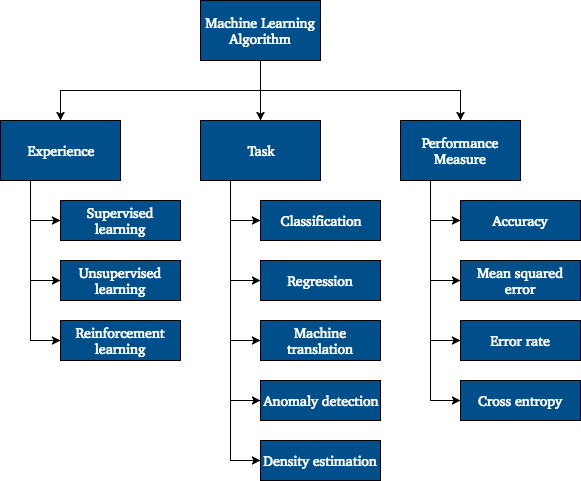
\includegraphics[height=10cm]{img/ml_classification}
  \caption{Classification dimensions of machine learning algorithms}
\label{fig:ml_classification}
\end{figure}

\paragraph{Task \textit{T}}

Machine learning is often used in settings where programs with fixed rules are
insufficient. Hence, the application of machine learning adds a more dynamic
component in order to perform a given task. Here, the task is usually to process
an \textit{example} which consists of a set of \textit{features}. Features are
attributes of an object that can be measured quantitatively~\cite{Goodfellow2016}. 
In the example described above, the number of bedrooms is one the features of 
the house object. The task \textit{T} would then be to predict a price for this 
house. Depending on the type of the specific output variable this problem can 
be assigned to one of many groups of tasks (see Fig.~\ref{fig:ml_classification}). If the output was an
exact price (e.g. 1,000,000\$), this would constitute a \textbf{regression} task. 
Assuming the goal is to assign the house to a price interval (e.g., (500,000\$, 1,000,000\$]),
one would describe this as a \textbf{classification} problem. Other common tasks
can be derived from Figure 2.1. One such example would be \textbf{anomaly detection}, e.g.,
if the goal were to detect expensive houses in a neighborhood where house prices
are typically low. The task could also be to translate house descriptions from
English into other languages (\textbf{machine translation}) or to derive an
estimation of the underlying probability distribution of the data (\textbf{density estimation}).

\paragraph{Performance measure \textit{P}}

In order to perform a task \textit{T} better over time, the algorithm needs
a quantitative measure for its current performance. In the setting of
house price prediction, the algorithm should get feedback on the quality of its
predictions. For a regression problem a suitable performance measure would be 
the \textbf{mean squared error} over all training examples. Possible measures
for classification tasks would be \textbf{accuracy} (i.e., how many examples
were classified correctly?) or the \textbf{error rate} (i.e., how many
examples were classified incorrectly?). If the algorithm outputs class 
probabilities, \textbf{cross entropy} can be used to evaluate model
performance. Defining the correct performance measure can be more difficult
for more complex learning problems such as machine translation. The design of 
\textit{P} can influence the training process, e.g., if not all errors have the
same misclassification cost. Furthermore, machine learning models should be evaluated on unseen
data, i.e., data points that were not used for training the model. This way,
one derives a better estimate of the generalization abilities of the model~\cite{Bishop2006, Goodfellow2016, Mitchell1997}.

\paragraph{Experience \textit{E}}

Machine learning algorithms can further be classified by the `kind of experience
they are allowed to have during the training process'~\cite[p. 104]{Goodfellow2016}.
In \textbf{unsupervised learning} settings the label for an example (also called
\textit{data point}) is unknown. For the house price prediction example this
would mean that real prices for the houses in the data set are not
available for training. Performing classification or regression tasks would
therefore not be feasible as the performance measure \textit{P} can not be
determined. Potential tasks in such an unsupervised learning setting would be
clustering (e.g., identifying similar houses), or performing density estimation
(e.g., to derive the probability for a given house price). In a broad sense these
kinds of algorithms aim to identify underlying distributions of data. Contrary, in 
\textbf{supervised learning} settings each example is associated with an 
observed output (usually called \textit{label} or \textit{target}). Hence, a
performance measure can be calculated for each data point, by which the
algorithm is able to improve its predictions over time (see above classification
and regression examples)~\cite{Goodfellow2016, Bishop2006}. The third kind of
experience for a machine learning algorithm is a \textbf{reinforcement learning}
setting. Here, the algorithm does not rely on a fixed data set, but instead 
interacts with its environment steadily. It then learns from the feedback it
derives from these interactions. A common usecase for reinforcement
learning is the interaction of agents with the real environments, e.g.,
self-driving cars. In most of these settings collecting all data points is
insufficient or simply not feasible~\cite{Sutton1998}.

It becomes obvious that the three dimesions are related, i.e., choices for a
specific dimension are conditioned on the other dimensions. Prior identification 
of all three dimensions is key in order to identify 
`well-defined learning problems'~\cite[p. 2f.]{Mitchell1997}. All developed 
learning algorithms in later chapters will also use this classification 
framework. 


\subsection{History}
\label{sub:dl_history}

After establishing the basic terminology for this thesis, 
it is now possible to take a closer look at the algorithm group of 
\textit{neural networks}. Therefore, this subsection will focus on historical
developments of neural networks, a group of algorithms that deep learning falls
into.
Understanding the origins of this methodology will be helpful in the next 
subsection which explains the more formal aspects of neural networks.
Overall, the history of neural network research is often separated into three
distinct phases of active research and progress in the literature~\cite{Goodfellow2016}.
All three phases will be described in the following.

\paragraph{Phase 1: First models}

The first forms of neural networks were developed in the 1940s, when
researchers tried to model learning machines inspired by the human brain.
The first such model was the McCulloch-Pitts neuron which constituted a linear
model:

\begin{equation}
  f (x, w) = w_1 x_1 + w_2 x_2 + \cdots + w_m x_m
\end{equation}

The neuron was able to recognize two different categories by determining
whether $f(x, w)$ was positive or negative~\cite{McCulloch1943}.
As a downside, there was no way to set the weights via an algorithm.
Instead, the weights had to be set by a human.
The first model of a neuron which overcame this obstacle was the \textit{perceptron}
developed by Rosenblatt~\cite{Rosenblatt1958}. The main contribution of the
perceptron was a simple algorithm to update weights iteratively.
The only requirement for the algorithm to run was a set of labeled examples.
In the same timespan, Widrow and Hoff~\cite{Widrow1960} came up with a similar
model called \textit{adaptive linear element (ADALINE)} for regression problems.
The main disadvantage that could not be overcome at the time lied in the 
linearity of the model which limited its representational capability.
For example, the model from equation 2.1 is not able to learn the XOR function 
(see equations 2.2 to 2.5)~\cite{Minsky1969}.

\begin{align}
  f ([0, 1], w) = 1\\
  f ([1, 0], w) = 1\\
  f ([0, 0], w) = 0\\
  f ([1, 1], w) = 0
\end{align}

These limitations caused a decline in research interest and thus mark the end
of the first phase of neural network research, which is often referred to
as \textbf{cybernetics}~\cite{Goodfellow2016}.

\paragraph{Phase 2: Backpropagation and connectionism}

The second wave of neural network research largely took place from the late
1970s until the mid-1990s. 
The problem of limited representational capability was overcome by wrapping
neurons inside a non-linear function, which basically transforms its output~\cite{Fukushima1975}.
This idea was combined with distributing the representational capacity over
more neurons, thus creating the first \textit{neural networks}. 
The neurons were combined in layers which were connected to each other.
This is also the main reason why this phase of neural network research is
often referred to as \textbf{connectionism}~\cite{Goodfellow2016}.
The intuition behind this was that more neurons would be more capable of
representing the input by acting together. 
Here, each neuron stands for a distinct feature, e.g., the color of an object
or the type of object itself~\cite{Rumelhart1986a}.
Training these more complex models became easier and faster with the
introduction of the backpropagation algorithm~\cite{Rumelhart1986}.
More complex neural networks meant more weights which needed to be updated
iteratively. 
The backpropagation algorithm is still the dominant approach for training
neural networks, because it offers a way of efficiently calculating the
updated weights.
The algorithm will be explained in more detail in the following subsection.
Despite the fast progress in academic research, the interest in neural networks
once again declined in the mid-1990s. The main reasons for this were the
lack of computational power to train deeper models containing more layers, as 
well as the advancements of other fields of machine learning (e.g., Support
Vector Machines) around this time~\cite{Goodfellow2016}.

% Third wave ("deep learning"):
% Training deep networks becomes efficient (Hinton 2006)
% Applications in many areas become possible (to be continued in Recent Developments)

\paragraph{Phase 3: Deep learning}

The difficulties of training deeper neural networks were overcome in 2006.
It was shown that a combination of more efficient training algorithms and
more advanced hardware enabled training deep networks in a reasonable amount of 
time~\cite{Hinton2006, Holden2006}.
Further developments in the techniques and availability of more computational
power led to popularization of deep neural networks and the term \textbf{deep
learning} was coined~\cite{Goodfellow2016, LeCun2015}.
Deep learning was used in models that outperformed other machine learning
algorithms in areas like image and speech recognition~\cite{Krizhevsky2012, Hinton2012}. 
These made use of neural network architectures like \textit{convolutional neural networks} 
and \textit{recurrent neural networks}, that were originally developed during 
the second wave of neural network research~\cite{Fukushima1980, Hochreiter1997, LeCun1998}.

Subsection 2.1.4 will go into more detail about the recent developments of
deep learning techniques. The following subsection will describe the basic
structure, elements and algorithms of neural network architectures in more
detail. This will ease the understanding of the more modern and complex
architectures and lay a mathematical foundation for the later chapters.


\subsubsection{Basic Concepts}
\label{sub:dl_concepts}

Understanding more sophisticated deep learning methods used in later
chapters requires comprehension of the basic concepts behind artificial
neural networks.
This chapter introduces mathematical foundations of both neural network
structure and algorithms.
The notation mostly follows the one from Nielsen~\cite{Nielsen2015}, but also
adds explanations from Bishop~\cite{Bishop2006} and Goodfellow et al.~\cite{Goodfellow2016}.
The first paragraph in this subsection will introduce the major elements
of the neural network training process which will then be described in more
detail in the following paragraphs.

\paragraph{Training process}

Like most machine learning algorithms, neural networks are trained using an iterative process.
In short, the network takes some example from the training data set as an input 
and calculates the respective output via a process called 
\textbf{forward propagation}.
Depending on the size of the data set, it repeats this procedure for more 
examples.
Since this constitutes a supervised learning problem, desired outputs for
each example are known.
These can be used to calculate the prediction error, which is determined by the
\textbf{cost function}.
The assessed error can then be used to calculate updates for the parameters of
the networks which are called \textit{weights}.
This process is known as \textbf{backpropagation}.
The examples which are used during one iteration of the training process are
called a \textit{mini-batch}.
A full run through all examples of the training data set is referred to as an
\textit{epoch}.
The forward and backpropagation algorithms and the cost function are the three
basic elements of an artifical neural network. 
In order to define them in more detail, mathematical notation has first to be
established.

\paragraph{Neural network structure}

\begin{figure}[h]
  \centering
  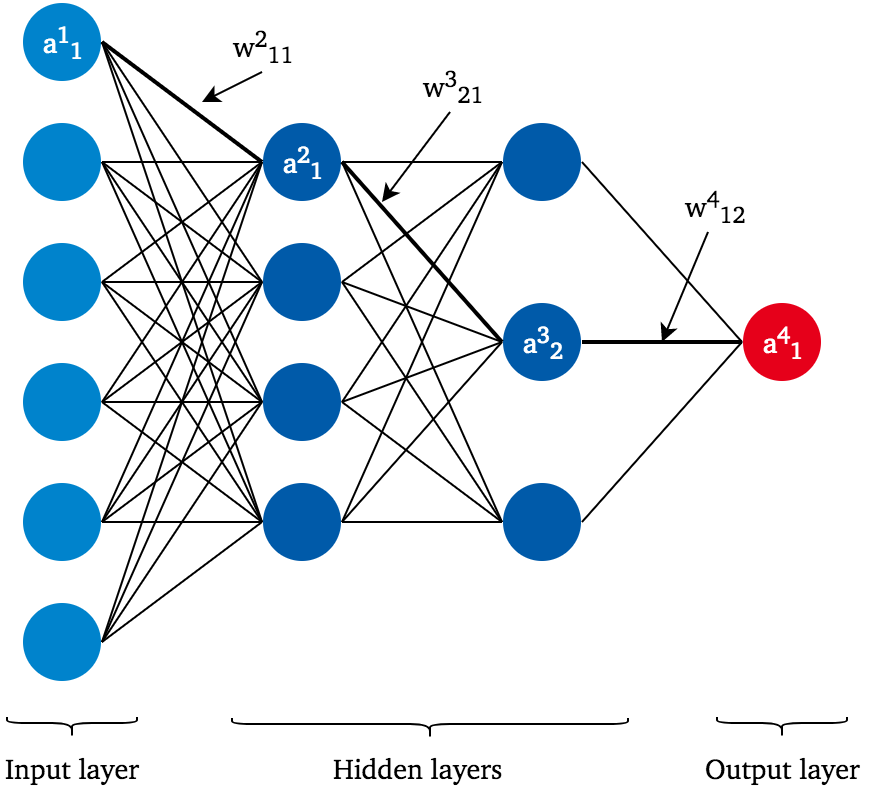
\includegraphics[height=10cm]{img/nn_architecture_2}
  \caption{Neural network structure and notation}
\label{fig:nn_architecture}
\end{figure}

Neural networks basically consist of nodes (also called \textbf{units}) which
are organized as layers.
The single layers of a neural network are wired together via edges that are
called \textbf{weights}.
This subsection will focus on the most basic architecture of a neural network,
called a \textbf{feed-forward network}.
In this architecture all units in a specific layer are connected to all units
in the following layer.
Such a layer is then referred to as being \textit{fully-connected}.
More sophisticated layer architectures will be introduced in subsection~\ref{sub:dl_developments}.
Figure~\ref{fig:nn_architecture} shows an example of a fully-connected network
that contains an input layer with six units, two hidden layers with four respective
three units and and an output layer containing one single unit.
Here, hidden layers are all layers between input and output layer.

In the following, $a_j^l$ will refer to the $j^{th}$ unit in the $l^{th}$ layer.
Weight $w_{jk}^l$ then stands for the weight which connects the $k^{th}$ unit in
the ${(l-1)}^{th}$ layer with the $j^{th}$ unit in the $l^{th}$ layer.
Figure~\ref{fig:nn_architecture} contains an example path from input to ouput
layer which resembles this notation.

\paragraph{Forward propagation}
\label{sub:dl_forward}

During the forward propagation process, the neural network calculates an output
for a specific input with respect to the current weights in the network.
Thus, the network can be written as a function $f(x,w)$ where $x$ is an input
vector or matrix and $w$ is the set of all weights for this network.
The units in the input layer receive their value from the input vector.
All units in later layers are calculated using equation~\ref{eq:activation}.

\begin{equation}
  \label{eq:activation}
  a_j^l = \sigma(\sum_k w_{jk}^l a_k^{l-1} + b_j^l)
\end{equation}

In this equation, $a_j^l$ is also called an \textbf{activation}, $\sigma$ is a
non-linear transformation function and $b_j^l$ is an added bias term.
The bias term is here independent of the activations in the previous layer.
In practice, this calculation can be parallelized for all activations in a layer
by rewriting it in matrix form (see equation~\ref{eq:activation_matrix}).

\begin{equation}
  \label{eq:activation_matrix}
  a^l = \sigma(w^l a^{l-1} + b^l)
\end{equation}

Here, $a^l$ is the vector of all activations in layer $l$, $b^l$ is the vector
of all bias terms in layer $l$ and $a^{l-1}$ is the vector of all activations
in the previous layer. The matrix $w^l$ resembles all connections from layer $(l-1)$
to layer $l$, where $w^l_{jk}$ is the entry in the $j^{th}$ row and $k^{th}$ column.
The function $\sigma$ is applied element-wise to the result vector.

%\outline{What are examples for non-linearities?}
\begin{figure}[h]
  \centering
  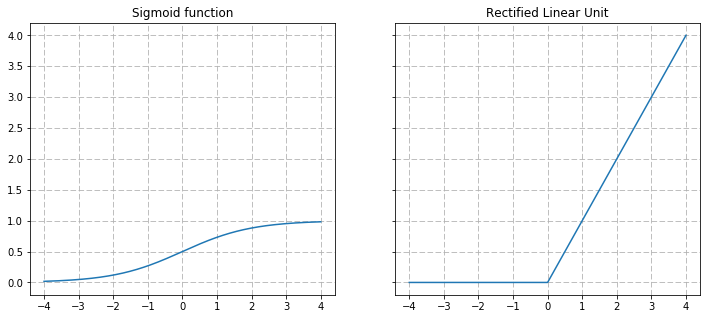
\includegraphics[height=7cm]{img/nn_activations}
  \caption{Popular neural network activation functions}
\label{fig:activations}
\end{figure}

If $\sigma(x) = x$, then the output activations $a^l$ will just be a linear
combination of the input activations $a^{l-1}$.
This property does obviously not change when applied over more layers.
The result will still be a linear function.
In contrast to that, if $\sigma$ is a non-linear function, the network receives more 
representational capability, i.e., it can learn to represent a bigger variety of 
functions. 
Two popular choices for $\sigma$ are the \textit{sigmoid function} and the
\textit{Rectified Linear Unit (ReLU)} (see figure~\ref{fig:activations}). 
The sigmoid function is given by equation~\ref{eq:sigmoid}, whereas ReLU is 
simply equal to the maximum of the input and zero (equation~\ref{eq:relu}).

\begin{equation}
  \label{eq:sigmoid}
  \sigma(x) = \frac{1}{1 + \exp(-x)}
\end{equation}

\begin{equation}
  \label{eq:relu}
  \sigma(x) = \max(0, x)
\end{equation}

Outputs of the sigmoid function are guaranteed to be between zero and one, which fits
the problem of predicting class probabilities.
Hence, the sigmoid function is most commonly applied in output layers of networks that
train on a classification task.
Contrary, most hidden layers in modern neural networks use ReLU as an activation
function.
The function was introduced in 2000 and has shown to be suitable for most deep
learning techniques, since it stabilizes the training process~\cite{Hahnioser2000, Nair2010}.

All in all, forward propagation is the layer-wise application of above described
calculations. For the example network in figure~\ref{fig:nn_architecture}, the
output for an example data point $x$ can be determined according to equation~\ref{eq:forward_prop}.
The enumerator in $\sigma$ indicates that different activation functions can
be applied in each layer.

\begin{equation}
  \label{eq:forward_prop}
  a^4 = \sigma^4(w^4 \sigma^3(w^3 \sigma^2(w^2 x + b^2) + b^3) + b^4)
\end{equation}

With the calculated outputs it is possible to evaluate predictions of the
networks by calculating the error according to the cost function.

\paragraph{Cost function}

In order to state necessary assumptions about the cost function, a first look
at the goal of the backpropagation algorithm is useful.
Backpropagation aims at deriving updates for all weights and biases in
the network.
It does so by calculating the gradients $\partial C / \partial w$ and 
$\partial C / \partial b$ of the cost function with respect to weights and
biases.
Two assumptions about the cost function have to be made, so that the 
backpropagation algorithm is able to work. 
The reasons for these assumptions will be explained in the next paragraph.
For illustration purposes this paragraph will use the \textit{quadratic cost function}
as a running example (see equation~\ref{eq:quad_costs}).
Here, $y(x)$ is the desired output for input $x$, $n$ resembles the number of
examples in the current mini-batch and $L$ denotes the output layer of the
network.

\begin{equation}
  \label{eq:quad_costs}
  C = \frac{1}{2n} \sum_x \Vert y(x) - a^L(x) \Vert^2
\end{equation}

The first assumption (equation~\ref{eq:cost_assump_1}) is that the cost function 
can be calculated as the average of all error terms for the current batch
of training examples. For example the quadratic cost function can be written in
this form, because $C_x = \frac{1}{2} \Vert y - a^L \Vert^2$.

\begin{equation}
  \label{eq:cost_assump_1}
  C = \frac{1}{n} \sum_x C_x
\end{equation}

Secondly, the cost function has to be a function of the network output $a^L(x)$
(see equation~\ref{eq:cost_assump_2}).
Obviously, this is given for the quadratic cost function since $a^L(x)$ is used
for determining the error and all other components are fixed parameters.

\begin{equation}
  \label{eq:cost_assump_2}
  C = C(a^L)
\end{equation}

With these assumptions set the next paragraph will explain how the
backpropagation algorithm derives gradients for the weight updates which enable
learning in the training process.

\paragraph{Backpropagation}
\label{sub:backprop}

As mentioned before, the backpropagation offers a way to calculate gradients
of the cost function with regard to weights and biases of the network.
Optimization algorithms such as gradient descent then make use of these 
gradients when determining weight updates since they intuitively represent
the rate of change of the cost function with respect to these learnable weights.
This paragraph will explain how the backpropagation algorithm works in detail.
Proofs are out of scope for this thesis and therefore omitted completely.

Some definitions are helpful for the further explanations. Firstly
$z^l$ is defined as an intermediate quantity which represents the weighted
inputs for neurons in layer $l$ (see equation~\ref{eq:weighted_input}).

\begin{equation}
  \label{eq:weighted_input}
  z^l \equiv w^l a^{l-1} + b^l \Rightarrow a^l = \sigma(z^l)
\end{equation}

Another useful intermediate quantity is $\delta_j^l$ which denotes the error
in the $j^{th}$ neuron in the $l^{th}$ layer. The error is defined in
equation~\ref{eq:neuron_error} as the partial gradient of the cost function
with respect to the weighted input to the neuron. Intuitively, if this value
is large (positively or negatively), the cost can be lowered by updating the 
weighted input in the opposite direction.

\begin{equation}
  \label{eq:neuron_error}
  \delta_j^l \equiv \frac{\partial C}{\partial z_j^l}
\end{equation}

The following explanation of the backpropagation algorithm is centered around
the four fundamental equations mentioned by Nielsen~\cite{Nielsen2015}.
Since the value of the cost function is known after the forward propagation
procedure, the first step of backpropagation is to calculate the error in the
output layer $L$.
Equation~\ref{eq:bp_1_comp} states how this is achieved for a single neuron,
whereas equation~\ref{eq:bp_1_mat} shows the matrix-based form for efficient
computation in practice. In this equation $\nabla_a C$ is the vector of all partial
derivatives $\partial C / \partial a_j^L$ and $\odot$ denotes the element-wise
multiplication of two vectors, known as the \textit{Hadamard product}.
For the previously introduced quadratic cost function, it would simply hold
that $\nabla_a C = (a^L -y)$.
This is also where the assumption about the cost function as a function of the
output activations $a^L$ comes into play.

\begin{equation}
  \label{eq:bp_1_comp}
  \delta_j^L = \frac{\partial C}{\partial a_j^L} \sigma'(z_j^L)
\end{equation}

\begin{equation}
  \label{eq:bp_1_mat}
  \delta^L = \nabla_a C \odot \sigma'(z^L)
\end{equation}

The expresssions can be split into two components. On the one hand, the partial
derivative represents the rate of change of the cost function with respect to
the output activations, on the other hand $\sigma'(z^L)$ determines how
fast the activation function changes for the weighted input.

After the error in the output layer is calculated, the next logical step is to
compute error terms for the previous layers.
In order to do that, the backpropagation algorithm only requires the error in
the next layer (see equation~\ref{eq:bp_2}).

\begin{equation}
  \label{eq:bp_2}
  \delta^l = ({(w^{l+1})}^T \delta^{l+1}) \odot \sigma'(z^l)
\end{equation}

The basic intuition behind this equation is that the known error $\delta^{l+1}$
flows backward through the network by multiplying it with the weight
matrix $w^{l+1}$.
It is then further moved through the activations of neurons in layer $l$ by
building the Hadamard product with the derivative of the activation function.
In summary, the first two equations offer a way to determine the errors for all
layers in the network.
The final two steps now aim to relate the errors to the partial derivatives
$\partial C / \partial w$ and $\partial C / \partial b$.

Equation~\ref{eq:bp_3} shows that the gradient of the cost function with respect
to any bias in the network is equal to the error at that neuron.
In short, this is also written as stated in equation~\ref{eq:bp_3_short}.

\begin{equation}
  \label{eq:bp_3}
  \frac{\partial C}{\partial b_j^l} = \delta_j^l
\end{equation}

\begin{equation}
  \label{eq:bp_3_short}
  \frac{\partial C}{\partial b} = \delta
\end{equation}

For weights, this computation is slightly more complex because they represent
a connection between two neurons.
In order to derive the gradient for a weight, the error in the current layer
has to be multiplied by the activation of the connected neuron in the previous
layer (see equation~\ref{eq:bp_4}).
This implies that weight updates are smaller if the input activation is near
zero.
Hence, the weight is said to \textit{learn slowly}.

\begin{equation}
  \label{eq:bp_4}
  \frac{\partial C}{\partial w_{jk}^l} = a_k^{l-1} \delta_j^l
\end{equation}

Optimization algorithms make use of the computed gradients in that they determine
updates for all weights and biases in the network.
Figure~\ref{fig:grad_desc} illustrates mechanics of most optimization
algorithms used in neural networks.
Here, a common practice is to use mini-batches, i.e., small collections of
examples, for each iteration of the algorithm.
For each example the output of the network is calculated, which is then used
to determine the output error. 
The error in the output layer is then propagated through the network in order
to compute the gradients for weights and biases.
In the final step of the iteration, the weights (including biases) are updated
according to the gradients.
The most basic optimization algorithm called \textbf{gradient descent} uses the
update formula in equations~\ref{eq:gd_update_weights} and~\ref{eq:gd_update_biases}.

\begin{equation}
  \label{eq:gd_update_weights}
  w^l \rightarrow w^l - \frac{\eta}{m} \sum_x \delta^{x,l}{(a^{x,l-1})}^T
\end{equation}

\begin{equation}
  \label{eq:gd_update_biases}
  b^l \rightarrow b^l - \frac{\eta}{m} \sum_x \delta^{x,l}
\end{equation}

It averages over the gradients determined by looking at single examples, which
is only possible through the first assumption about the cost function (see equation~\ref{eq:cost_assump_1}).
Here, $m$ is the number of examples in the batch and $\eta$ resembles the
\textit{learning rate} which is a hyperparameter that has to be set prior to
learning.

\begin{figure}[h]
  \centering
  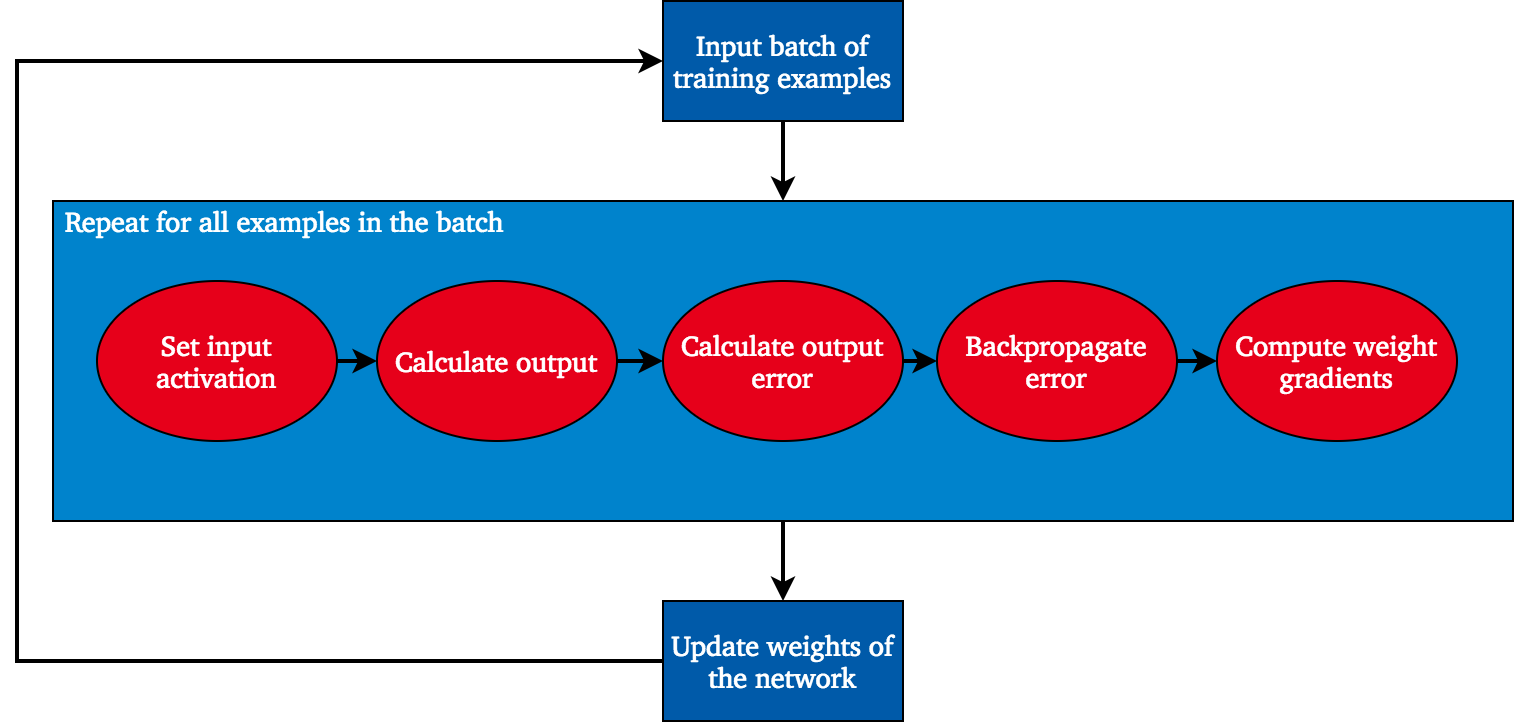
\includegraphics[height=8cm]{img/nn_optimization_3}
  \caption{Optimization in neural networks}
\label{fig:grad_desc}
\end{figure}

All in all, the choice of activation function and optimization algorithm largely
influences efficiency and stability of the learning process.
More sophisticated optimization algorithms will be introduced in the next
subsection, along with recent advances regarding architectures and
regularization techniques.


\subsubsection{Recent Developments}
\label{sub:dl_developments}

After basic paradigms of training neural networks were introduced in the last
subsection, this chapter dives deeper into more sophisticated approaches
which were developed in the last years of deep learning research.
Therefore, the first part explains the drivers behind current progress in the
field (ch.~\ref{sub:dl_drivers}). More complex network architectures which enable
broader practical application will be discussed afterwards (ch.~\ref{sub:dl_architectures}),
before the remaining sections describe modern approaches to optimization
(ch.~\ref{sub:dl_optimization_algos}) and regularization of the training process
(ch.~\ref{sub:dl_regularization}).

\paragraph{Drivers}
\label{sub:dl_drivers}

Progress in deep learning research is mainly enabled by two factors, namely
increased data availability and improved hardware for computation.
Both factors will be detailed in the following.

The term \textbf{big data} is used to describe the phenomenon of increased data
availability.
Main causes for this are migration of transactions from the physical world
to the internet, wide spread of mobile devices like smartphones and success
of social networks, e.g., \textit{Facebook} and \textit{Twitter}.
Big data can best be described by the three dimensions volume, velocity and
variety, also known as the \textit{Three V's}.
Here, \textbf{volume} describes increases in created data, mainly over the 
internet. 
Where volume refers to total size of data sets, \textbf{velocity} stands for the
speed-up in data access. More and more data can be consumed in (nearly) real-time,
e.g., over streaming interfaces.
In addition, big data comes in more diverse form, which is where the \textbf{variety}
dimension has to be regarded.
User-generated images and videos, as well as sensor or GPS data from smartphones
are examples for data types which complement more traditional text and relational
data.
Companies making use of big data in the form of data-driven decision making
have been shown to be more profitable and productive than companies that do not
apply such practices~\footcite{McAfee2012}.
Modern world connectedness makes it possible to store data coming from
many different sources and process it in centralized manner, e.g., to offer
individualized services for consumers~\footcite{Jordan2015}.
Deep learning profits from big data, particularly because models become more
precise with larger data sets.
Large data sets have been shown to improve model performance more than careful
feature engineering, which is required for most machine learning algorithms~\footcite{Goodfellow2016}.
This trend is exemplified in growing benchmark data sets for deep learning
models.
For example, the \textit{MNIST} data set contains 70,000 images of size 28$\times$28 
pixels and served as a benchmark for image recognition since being first
introduced in 1998~\footcite{LeCun1998}.
Nowadays, the most commonly used benchmark for the same task is the \textit{ImageNet}
database, which consists of about 1.2 million images in higher 
resolution~\footcite{Russakovsky2015}.

Processing larger data sets demands a higher number of necessary computations.
Hence, \textbf{computational resources} have to evolve in order to calculate models
in a timely manner.
Deep learning models are most commonly trained using \textit{graphics processing
units} (GPUs), which were formerly applied to highly parallelized processing
in computer games.
GPUs are preferred over CPUs for these tasks, because they contain more
processing units which can carry out computations in parallel.
Graphics processors enable training of more complex models, i.e., models which
contain more neurons and thus learn representation with higher numbers of 
parameters~\footcite{Goodfellow2016, Raina2009}.

\begin{figure}[h]
  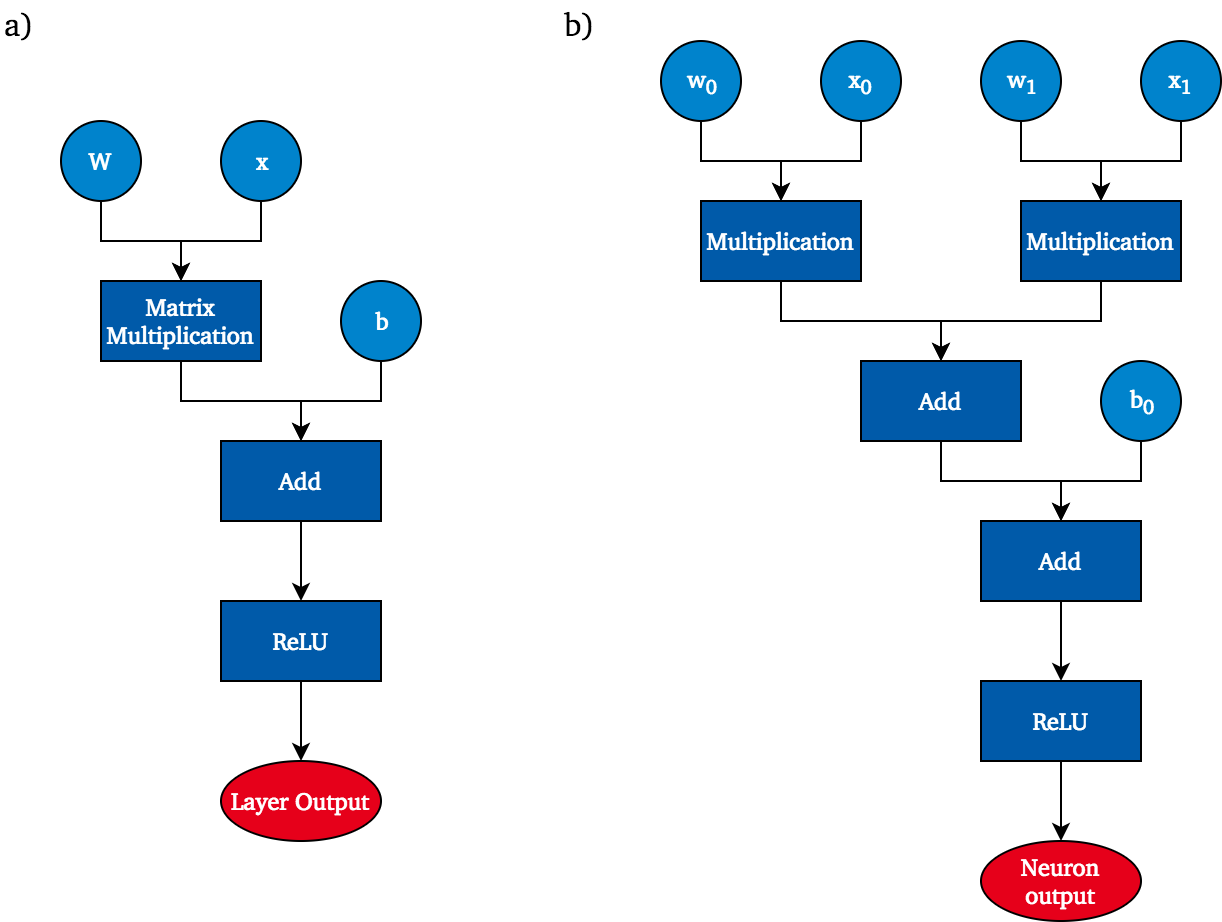
\includegraphics[height=10cm]{img/computation_graph_3}
  \caption[Computation graph for single layer and neuron]{Left: computation graph for a single layer \\ Right: computation graph for a single neuron}
\label{fig:comp_graph}
\end{figure}

Modern deep learning frameworks such as \textit{TensorFlow}\footnote{\url{https://www.tensorflow.org/}}
make use of GPUs by computing neuron outputs for a single layer in parallel.
Forward and backward propagation can be visualized using \textbf{computation
graphs}, which exemplify the single operations for calculating layer outputs.
Figure~\ref{fig:comp_graph}a shows a computation graph for the forward
pass through a fully-connected layer, as introduced in chapter~\ref{sub:dl_forward}.
Instead of computing the matrix operations on a single processing unit, the
calculation can be broken down into less complex subtasks.
Figure~\ref{fig:comp_graph}b exhibits the computation of a single neuron output
from a two-dimensional input vector $x$, which is obviously independent of
other activation computations in the same layer.
Most notably, matrix operations are replaced with element-wise calculations here.
Deep learning software typically computes forward and backward pass in this way
layer by layer in order to speed up the training process~\footcite{Abadi2016}.

This work applies modern deep learning software and hardware for its model.
Exact specifications can be found in chapter~\ref{ch:methodology}.

\paragraph{Network architectures}
\label{sub:dl_architectures}

Above described drivers enable training of more complex models for various
tasks.
In detail, these models contain more parameters and thus possess higher
representational capability.
Over decades of neural network reserach, specialized architectures have been
developed for tasks like image or speech recognition.
This subsection will present three network architectures, two of which will
be used for the model of this work.
For better understanding the architectures are compared to the basic fully-
connected model from chapter~\ref{sub:dl_concepts}

\begin{figure}[h]
  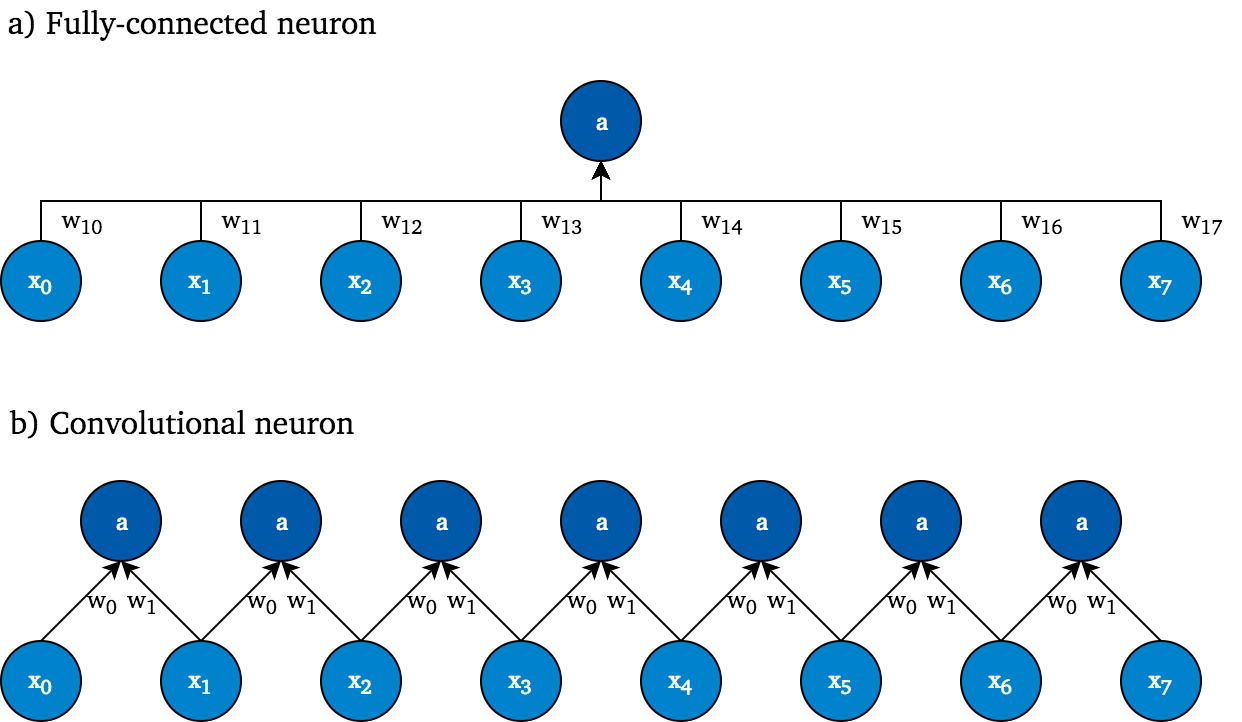
\includegraphics[height=8cm]{img/conv_layer.png}
  \caption{Comparison of fully-connected and convolutional neuron}
\label{fig:conv_layer}
\end{figure}

\textbf{Convolutional neural networks} were first developed by LeCun et al. in 1998,
based on approaches that had been invented during the 1980s~\footcite{Fukushima1980, LeCun1998}.
At that time they were mostly used for simple image processing tasks like
automatic character recognition from handwriting.
In order to understand what characterizes convolutional layers, it is helpful
to compare them to fully-connected layers.
Figure~\ref{fig:conv_layer} compares both layer types for a one-dimensional
input vector and a single neuron in the network layer.
In a fully-connected layer, all inputs are connected to the same neuron.
Contrary, in a convolutional layer, a fixed number of neighboring inputs (two in this example)
are connected to a neuron copy.
All neuron copies share the same weights, as denoted in Fig.~\ref{fig:conv_layer}b,
and thus learn a shared representation of some pattern.
For convolutions to make sense, the ordering of inputs has to be relevant.
This is the case for several data types, e.g., image, text or speech data.
Images will be used as an example here, because the effects of applying
convolutions can be visualized.
Intuitively, one can imagine a convolution as a neuron that is moved over the
vector of inputs and looks for one specific pattern.
For images, a convolution can thus be thought of as a filter that represents
a common reoccuring visual theme.
What kind of pattern (also called \textit{filter}) is learned by the neuron is
determined during the training process.

\begin{figure}[h]
  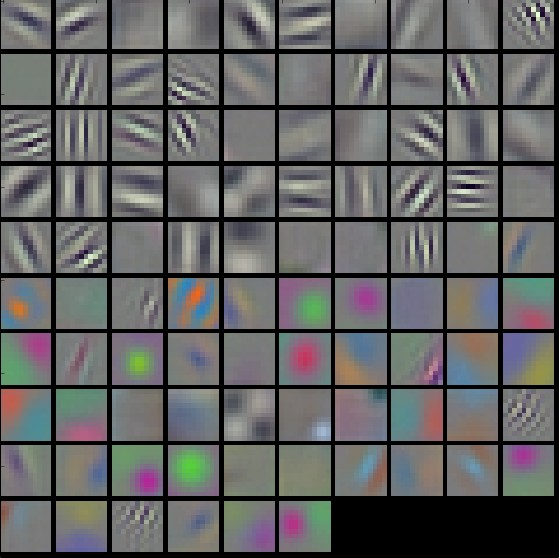
\includegraphics[height=8cm]{img/conv_filters.jpeg}
  \caption[Example filters in a convolutional layer]{Example filters in a convolutional layer~\footcite{Krizhevsky2012}}
\label{fig:conv_examples}
\end{figure}

Figure~\ref{fig:conv_examples} shows examples for such filters, as found in
a large convolutional neural network~\footcite{Krizhevsky2012}.
The top half of filters identify edges of varying orientation and thickness,
whereas the bottom half of filters focuses on color contrasts.
These are examples for filters learned in the first convolutional layer of a
network, that set a new benchmark for image recognition tasks.

\begin{figure}[h]
  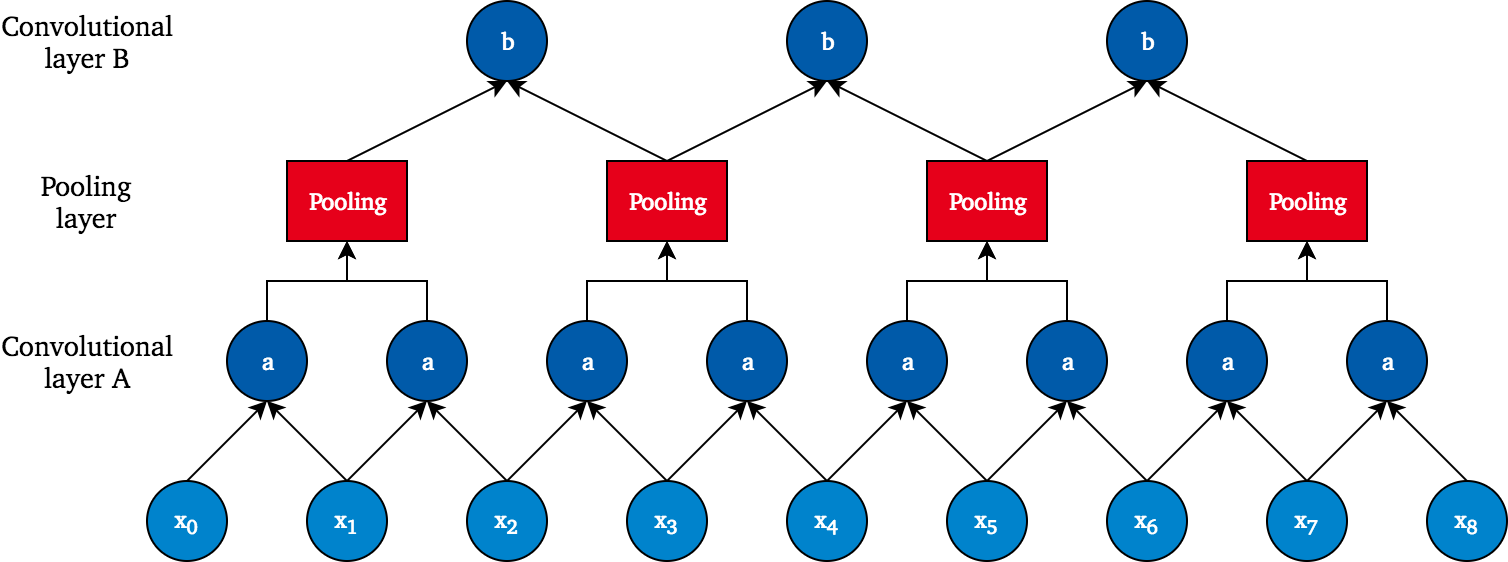
\includegraphics[height=6cm]{img/conv_architecture}
  \caption{Convolutional neural network}
\label{fig:cnn_architecture}
\end{figure}

In practice, convolutional layers are stacked, so that later layers can learn
to identify increasingly complex shapes, e.g., faces or objects, from more
primitive shapes like edges and color contrasts~\footcite{Simonyan2015}.
\textit{Pooling layers} are often used to combine the output of neuron copies, which
enables the next convolutional layer to detect shapes from a greater portion of
the image effectively.
This effect is visualized in Fig.~\ref{fig:cnn_architecture}, where the first
neuron copy of layer $B$ learns a filter from the output of two neuron copies
of layer $A$.
As an example, if layer $A$ learns to detect a horizontal edge, layer $B$ can
find occurrences of two parallel edges in an image.

As mentioned before, convolutional neural networks are mostly applied to data
like images and texts.
More details about practical applications will be discussed in chapter~\ref{sub:dl_applications}.

Like convolutional neural networks, \textbf{recurrent neural networks} (RNNs) are usually
used on data that underlies some kind of ordering.
Popular applications of RNNs lie in the  area of \textbf{Naturual Language
Processing (NLP)}, because text can be formalized as an ordered sequence of
words.

\begin{figure}[h]
  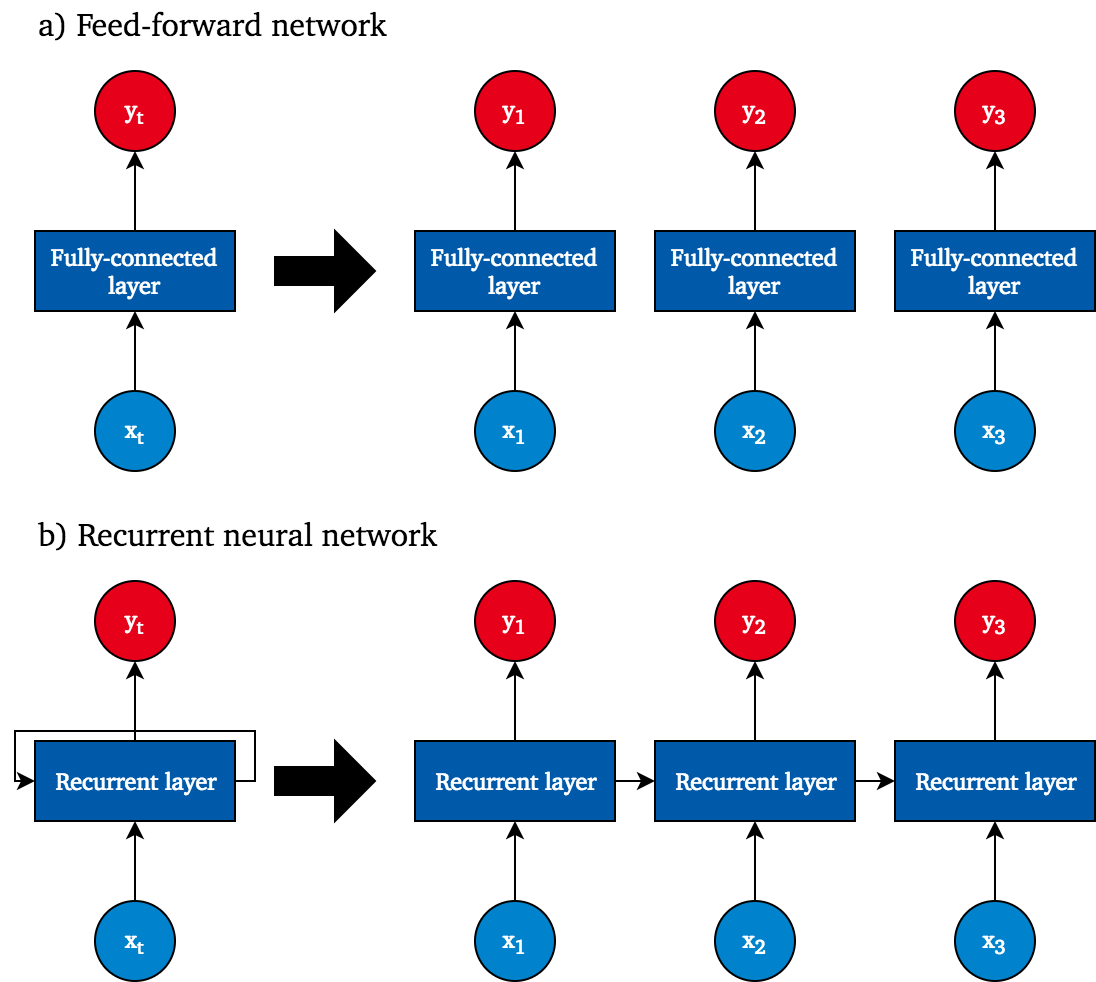
\includegraphics[height=10cm]{img/rnn_unrolled_2}
  \caption{Comparison between unrolled feed-forward and recurrent neural network}
\label{fig:rnn_unrolled}
\end{figure}

One drawback of basic feed-forward networks (see chapter~\ref{sub:dl_concepts})
when looking at ordered sequences is the lack of persistence between single
iterations.
Thus, when looking at an example $x_t$ the network does not know about previous
examples, e.g., $x_{t-1}, x_{t-2},\cdots$.
This fact is exemplified in Fig.~\ref{fig:rnn_unrolled}a, which unrolls a
feed-forward network containing one fully-connected layer into single iterations.
Intuitively, knowing about formerly observed events is useful in many use cases,
e.g., translation tasks or time-series forecasting.
Recurrent neural networks overcome the liability by introducing the concept
of \textbf{memory}.
As shown in Fig.~\ref{fig:rnn_unrolled}b, information is passed between
iterations, which for example enables the network to memorize previous inputs~\footcite{Goodfellow2016}.
The most applied RNN variant is the so-called \textbf{Long Short-Term Memory}
network, which will be explained in the following.

\begin{figure}[h]
  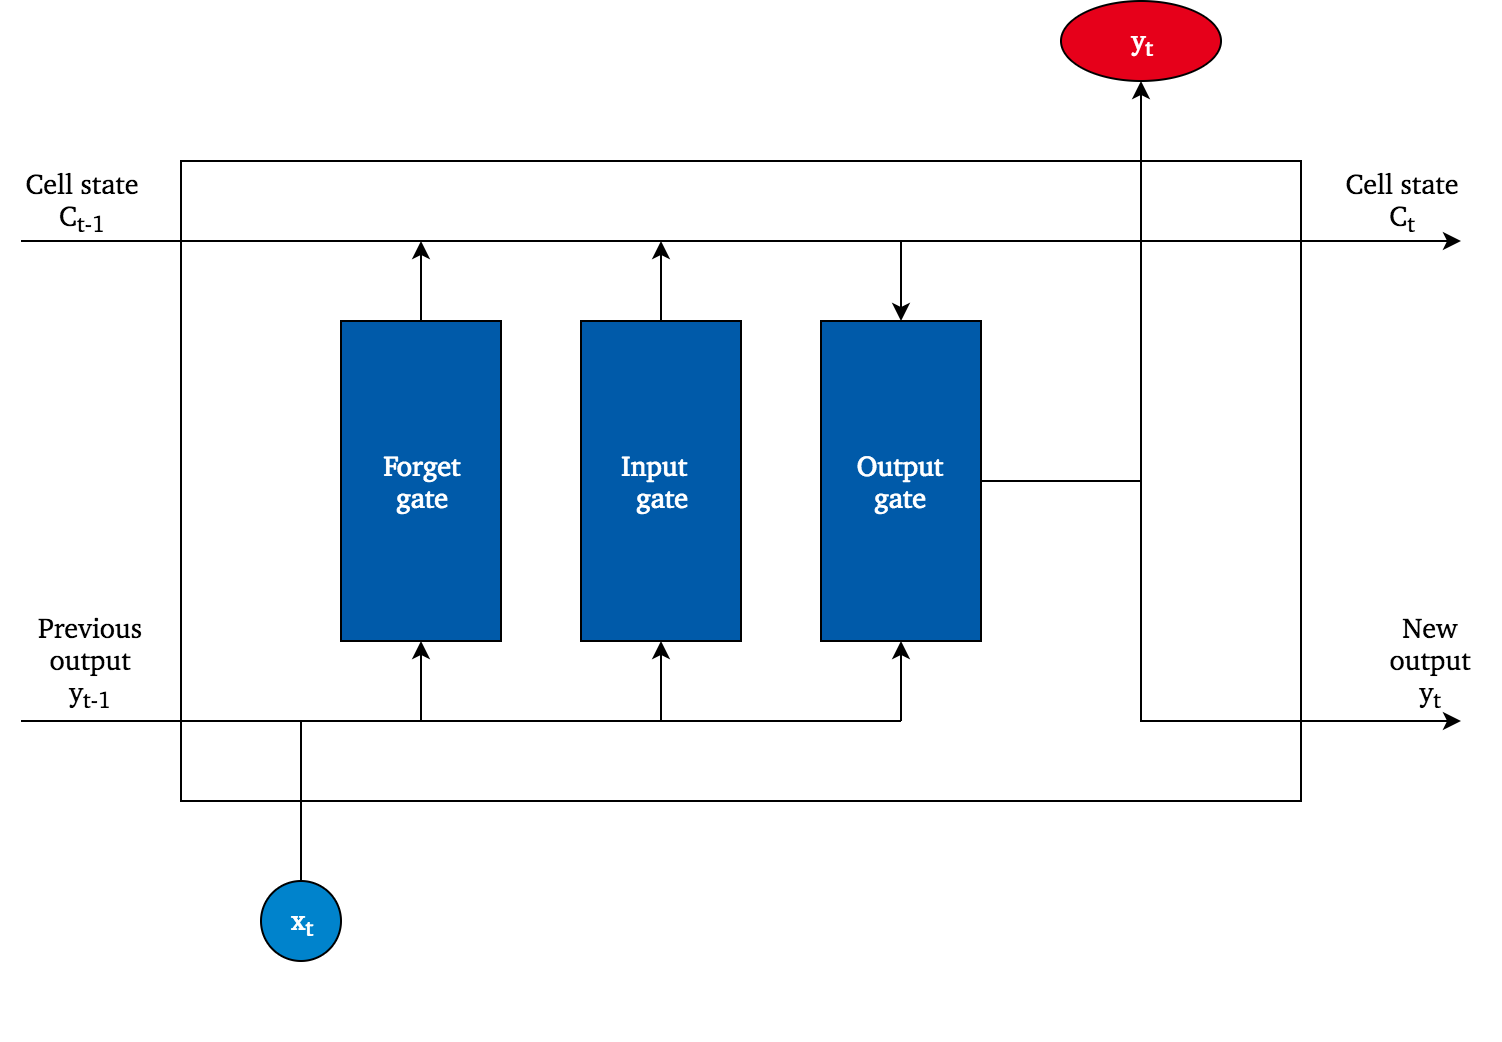
\includegraphics[height=11cm]{img/lstm_cell}
  \caption{Simplified LSTM cell}
\label{fig:lstm_cell}
\end{figure}

The Long Short-Term Memory (LSTM) network was first introduced by Hochreiter \&
Schmidhuber~\footcite{Hochreiter1997} in 1997, aiming to solve the problem of
storing information in a neural network over time.
A LSTM neuron (often calledLSTM cell) comprises four separate layers which 
manipulate the \textit{cell state}.
The cell state stores information and is passed between iterations of the
training process.
In summary, the four included layers serve three purposes: removing unnecessary
information, adding new information and creating an output.
The three tasks are handled in \textit{gates} which contain the necessary
network layers for computation and are responsible for editing the cell state
accordingly.
The following explanations of LSTM gates are illustrated in Fig.~\ref{fig:lstm_cell}.

All three gates process the current input $x_t$ and the output of the previous
iteration $y_{t-1}$.
LSTMs are commonly applied for Natural Language Processing tasks such as
language modeling, i.e., prediction of the next word based on previously seen
text.
Therefore, an example language modeling task will be used to describe the
gate functionalities~\footcite{Olah2015}.
Firstly, the \textit{forget gate} decides which information can be removed from
the cell state.
Internally, the forget gate contains a simple layer with sigmoid activations.
Outputs of the layer are multiplied element-wise with the cell state.
The activations are guaranteed to be between zero and one, where zero represents
`forgetting' and one stands for `keeping' information.
For example, when trying to predict words in a sequence it is necessary
to know about the current subject in order to conjugate an upcoming predicate
correctly.
If the current input $x_t$ represents a new subject, e.g., `he',the old subject should
probably be removed from the cell state in the forget gate.
Secondly, the \textit{input gate} is responsible for adding new information to the cell
state.
It does so in two distinct steps, which are processed in separate layers.
Here, the first decision is which information to update, and the second one
which new values to add.
The layer outputs are combined using the Hadamard Product and then added to the
cell state.
Continuing previous example, the input gate would likely add information about
the gender of the new subject, which determines word endings for predicates in
many languages.
Finally, an output for the current iteration is generated in the \textit{output gate}.
The output represents `a filtered version'~\footcite{Olah2015} of the cell state, e.g.,
information for upcoming verbs when a new subject is observed.
This happens through the use of another layer with sigmoid activations which
intuitively filters relevant information from the cell state.
As can be seen in Fig.~\ref{fig:lstm_cell}, the output is also passed to the
next iteration.

LSTMs have been applied to problems ranging from speech recognition to
image captioning, which require storing input information with regard to the
training process.
Architectures using multiple, stacked LSTM layers are also used in practice,
mainly to learn even more complex representations.
Detailed use cases will be a central theme in Ch.~\ref{sub:dl_applications}.

The previously described architectures of CNNs and RNNs were developed prior to
the third wave of neural network research and became efficiently trainable
due to driving factors described in Chapter~\ref{sub:dl_drivers}.
Finally, this subsection introduces \textbf{Generative Adverserial Networks (GANs)}, which
represent a more recently invented model architecture.
The basic concept was presented by researchers in 2014, and has gained popularity
since then~\footcite{Goodfellow2014}.
As can be extracted from the name, GANs belong to the family of \textit{generative
models}.
In contrast to \textit{discriminative models} which learn a decision boundary
between classes (e.g., Support Vector Machines), generative models implicitly 
model the probability distribution of inputs and outputs~\footcite{Bishop2006}.
Therefore, generative models can be used to generate new data from the learned
distribution, e.g., new images can be created from a sample of real images.
Generative adversarial networks approach this problem by combining two neural 
networks into a single model, as illustrated in Fig.~\ref{fig:gan_architecture}.

\begin{figure}[h]
  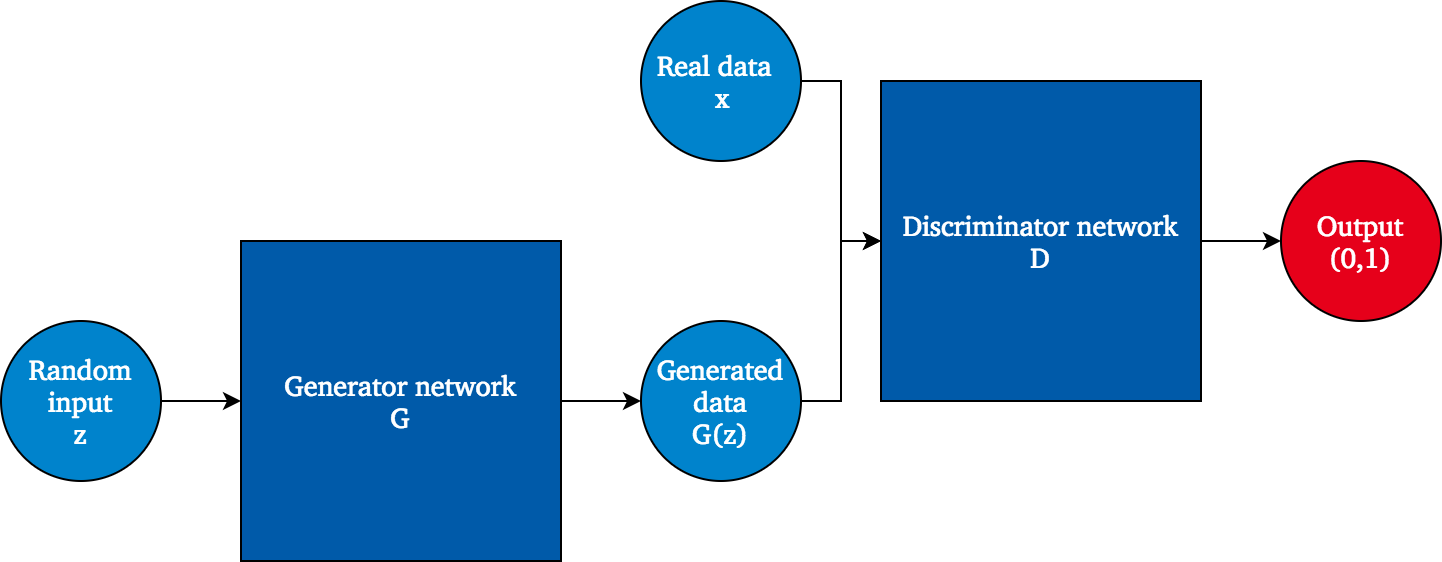
\includegraphics[height=6.5cm]{img/gan_architecture}
  \caption{Architecture of a Generative Adversarial Network (GAN)}
\label{fig:gan_architecture}
\end{figure}

In general, a GAN consists of a \textit{generator network G} and a \textit{discriminator network D}.
The generator outputs new data $G(z)$ from a random input vector $z$ which is
drawn from a normal distribution.
The generated data then serves as an input to the discriminator, along with
real data $x$.
Tasked with distinguishing between real and generated data, the discriminator
outputs probabilities representing an estimation of the authenticity of an
example.
Intuitively, the aim of the GAN architecture is to create new samples that carry
such similarity with original samples, that the discriminator can not differentiate
between real and generated anymore.
The question arises, how this objective can be expressed in a cost function.
Traditionally, generative models were trained by minimizing the distance of
generated output to nearest sample in the real data~\footcite{Goodfellow2014}.
GANs use a different objective function, which is exemplified in equation~\ref{eq:gan_obj}.

\begin{equation}
  \label{eq:gan_obj}
  \min_G \max_D V(D, G) = \mathbb{E}_{x \sim p_{data}(x)}[\log D(x)] + \mathbb{E}_{z \sim p_z (z)}[\log (1 - D(G(z)))]
\end{equation}

The cost function includes the objectives of both networks, as the generator
tries to minimize the above equation and the discriminator aims to maximize it.
Both terms represent in the equation represent log-likelihood functions.
Maximizing the equation means assigning the correct labels to data samples (aim
of the discriminator), minimizing it implies that the discriminator is not capable
of specifying where a sample comes from (aim of the generator).
The authors of the original paper prove the existence of a unique solution, where
the generator is able to represent the original data distribution and the 
discriminator outputs probabilities of 0.5 for every sample~\footcite{Goodfellow2014}.
Such a game between two entities following conflictive objectives is referred to
as a \textit{minimax setting}~\footcite{Russell1995}.

During the training process, weights for both networks have to be updated.
This can be achieved through backpropagating errors through both networks,
although some adaptations have to be made.
Training processes as follows:

\begin{enumerate}
  \item Determine architecture for generator and discriminator network
  \item Update $D$ while $G$ is not trainable and samples are split between real and generated
  \item Update $G$ while $D$ is not trainable and samples are all generated
  \item Repeat steps 2 and 3 for desired number of iterations
\end{enumerate}

It becomes obvious that the two networks are updated alternatively.
An important caveat is that one network is not trainable, i.e., the weights are
fixed, while the other one is updated.
Fixed weights are not updated during training, but solely used to pass information
forward and backward through the network.

GANs were applied to creation of images in the original paper, but have been
used for a bigger variety of problems since. As for the other architectures,
more practical applications can be found in Ch.~\ref{sub:dl_applications}.
After examining more advanced architectures, the next two subsections will
focus on the training process.
In particular, developments in optimization algorithms and regularization
techniques are described.

\paragraph{Optimization algorithms}
\label{sub:dl_optimization_algos}

The choice of optimization algorithms influences the stability of the training
process.
Here, the aim is to converge to a good solution in reasonable time, ideally
finding a minimum for the cost function by adapting weights in the network.
Chapter~\ref{sub:backprop} introduced a basic structure for optimization
algorithms in neural network training, as well as update functions for the
\textit{stochastic gradient descent} optimization algorithm.
Basically, gradient descent only relies on derived gradients and a hyperparameter
representing the learning rate, i.e., the step size towards a possible minimum
(~\ref{eq:gd}).
For complex neural networks, gradient descent can be hard to utilize effectively.
Suitable, often manual weight initialization and adaptions of the learning rate
during training are needed in order to derive good solutions.
More sophisticated optimization algorithms, which were developed in the last
years, overcome these limitations.
This subsection will first introduce the concept of \textit{momentum} in
numerical optimization and then explain a commonly deployed algorithm called
\textit{Adam}.

\begin{equation}
  \label{eq:gd}
  w_{t+1} \rightarrow w_t - \eta \nabla f(w_t)
\end{equation}

The concept of \textbf{momentum} was developed in the 1960s and has since been applied
to numerical optimization problems~\footcite{Polyak1964}.
During the third wave of neural network research, the concept was first
utilized for accelerating training processes in deep networks~\footcite{Sutskever2013}.
In its essence, momentum (equation~\ref{eq:momentum}) adds an additional step to 
the gradient descent update function (equation~\ref{eq:gd}).

\begin{align}
  \label{eq:momentum}
  v_{t+1} \rightarrow \mu v_t + \eta \nabla f(w_t) \\
  w_{t+1} \rightarrow w_t - v_{t+1}
\end{align}

The weight update $v_{t+1}$ is composed by two terms: the gradient $\nabla f(w_t)$
weighted with the learning rate $\eta$ and the previous update $v_t$ multiplied
with the \textit{momentum coefficient} $\mu$.
Therefore, the update in iteration $t+1$ depends on the update of iteration $t$,
which again is dependent on $v_{t-1}$ and so on.
The added term $\mu v_t$ can thus be interpreted as an exponentially moving 
average of previous updates, where hyperparameter $\mu$ determines the magnitude 
of influence of these predecessor updates.
Momentum allows the optimizer to progress more evenly without too many changes
of direction.
This overcomes the liability of gradient descent which is susceptible to
frequent changes of directions in the gradient, e.g., if examples in a mini-batch
are particularly noisy.

As outlined in above paragraph, momentum keeps track of the exponentially moving
average of previous gradients.
This added average constitutes a first moment estimate of the gradients, also 
known as \textit{mean estimate}.
The \textbf{adaptive moment estimation (Adam)} optimization algorithm enhances
momentum with further computations in order to guarantee accelerated
convergence~\footcite{Kingma2014a}.
Intuitively, Adam adapts the learning rate for each parameter based on mean and
variance of recent updates in the specific parameter.
Equations~\ref{eq:adam_start} through~\ref{eq:adam_end} exemplify the update
computation for a single parameter $w$ in iteration $t$.

\begin{align}
  g_t &= \nabla f(w_t) \label{eq:adam_start} \\
  m_t &= \beta_1 m_{t-1} + (1-\beta_1) g_t \label{eq:adam_2} \\
  v_t &= \beta_2 v_{t-1} + (1-\beta_2) g_t^2 \label{eq:adam_3} \\
  \widehat{m}_t &= \frac{m_t}{1-\beta_1^t} \label{eq:adam_4} \\
  \widehat{v}_t &= \frac{v_t}{1-\beta_2^t} \label{eq:adam_5} \\
  w_{t+1} &= w_t - \frac{\eta}{\sqrt{\widehat{v}_t} + \epsilon} \widehat{m}_t \label{eq:adam_end}
\end{align}

Equations~\ref{eq:adam_2} and~\ref{eq:adam_3} compute mean and
uncentered variance estimates of the gradient, similar to momentum.
$\beta_1$ and $\beta_2$ are hyperparameters, whose default values are $0.9$ and
$0.999$ respectively.
Because of these defaults and zero initialization of $m$ and $v$, the estimates
are biases towards zero, especially in early iterations.
This bias is corrected in equations~\ref{eq:adam_4} and~\ref{eq:adam_5}, where
the scaling factor $\frac{1}{1-\beta_1^t}$ is larger for smaller values of $t$
and therefore accounts for smaller values of the estimates as a result of 
zero initialization.
Final updates are then calculated via the corrected estimates and hyperparameters
$\eta$ (representing the learning rate) and $\epsilon$ (defaults to $10^{-8}$).

\begin{figure}[h]
  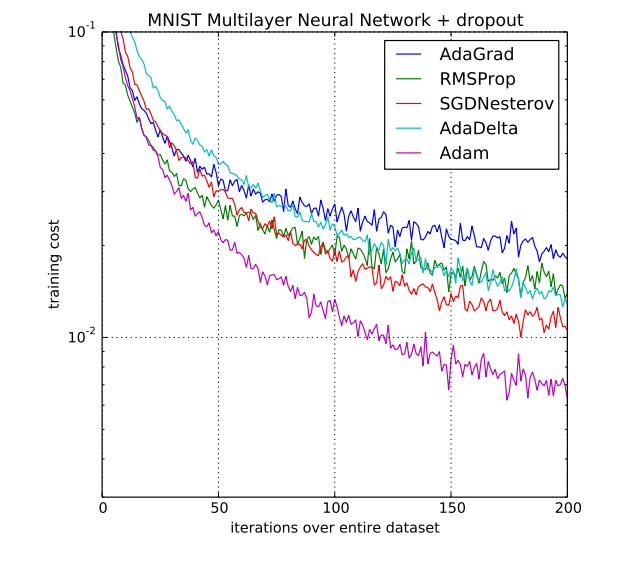
\includegraphics[height=10cm]{img/adam_comparison}
  \caption[Comparison of optimization algorithms]{Comparison of optimization algorithms~\footcite{Kingma2014a}}
\label{fig:adam_comp}
\end{figure}

Kingma \& Ba~\footcite{Kingma2014a} list concise implementation, computational efficiency,
suitability for complex models with many parameters and reasonable default values
for the hyperparameters as main benefits of adaptive moment estimation.
Figure~\ref{fig:adam_comp} compares Adam to other optimization algorithms,
applied in the context of a deep neural network with the task of handwriting
recognition.
It can be seen that Adam achieves a better solution, i.e., lower value of the
cost function, over the course of 200 iterations.

\paragraph{Regularization techniques}
\label{sub:dl_regularization}

In addition to optimization algorithms, regularization techniques largely
influence training process stability and generalization ability of the
resulting model.
These techniques are particularly helpful for complex models such as deep
neural networks, and custom methods have been developed during the current
research wave.
This subsection will introduce regularization procedures after firstly explaining
the concept of overfitting which many techniques aim to prevent.

\textit{Generalization} constitutes the main challenge in machine learning and
denotes the ability to `perform will on new, previously unseen inputs'~\footcite[110]{Goodfellow2016}.
Therefore, machine learning models should not only be evaluated using training
error, i.e., the performance measure on training data, but also via \textit{test
error}, i.e., the performance on unseen test data.
In summary, key objectives of machine learning algorithms can be put as follows:

\begin{enumerate}
  \item Minimize training error
  \item Minimize gap between training and test error
\end{enumerate}

\begin{figure}[h]
  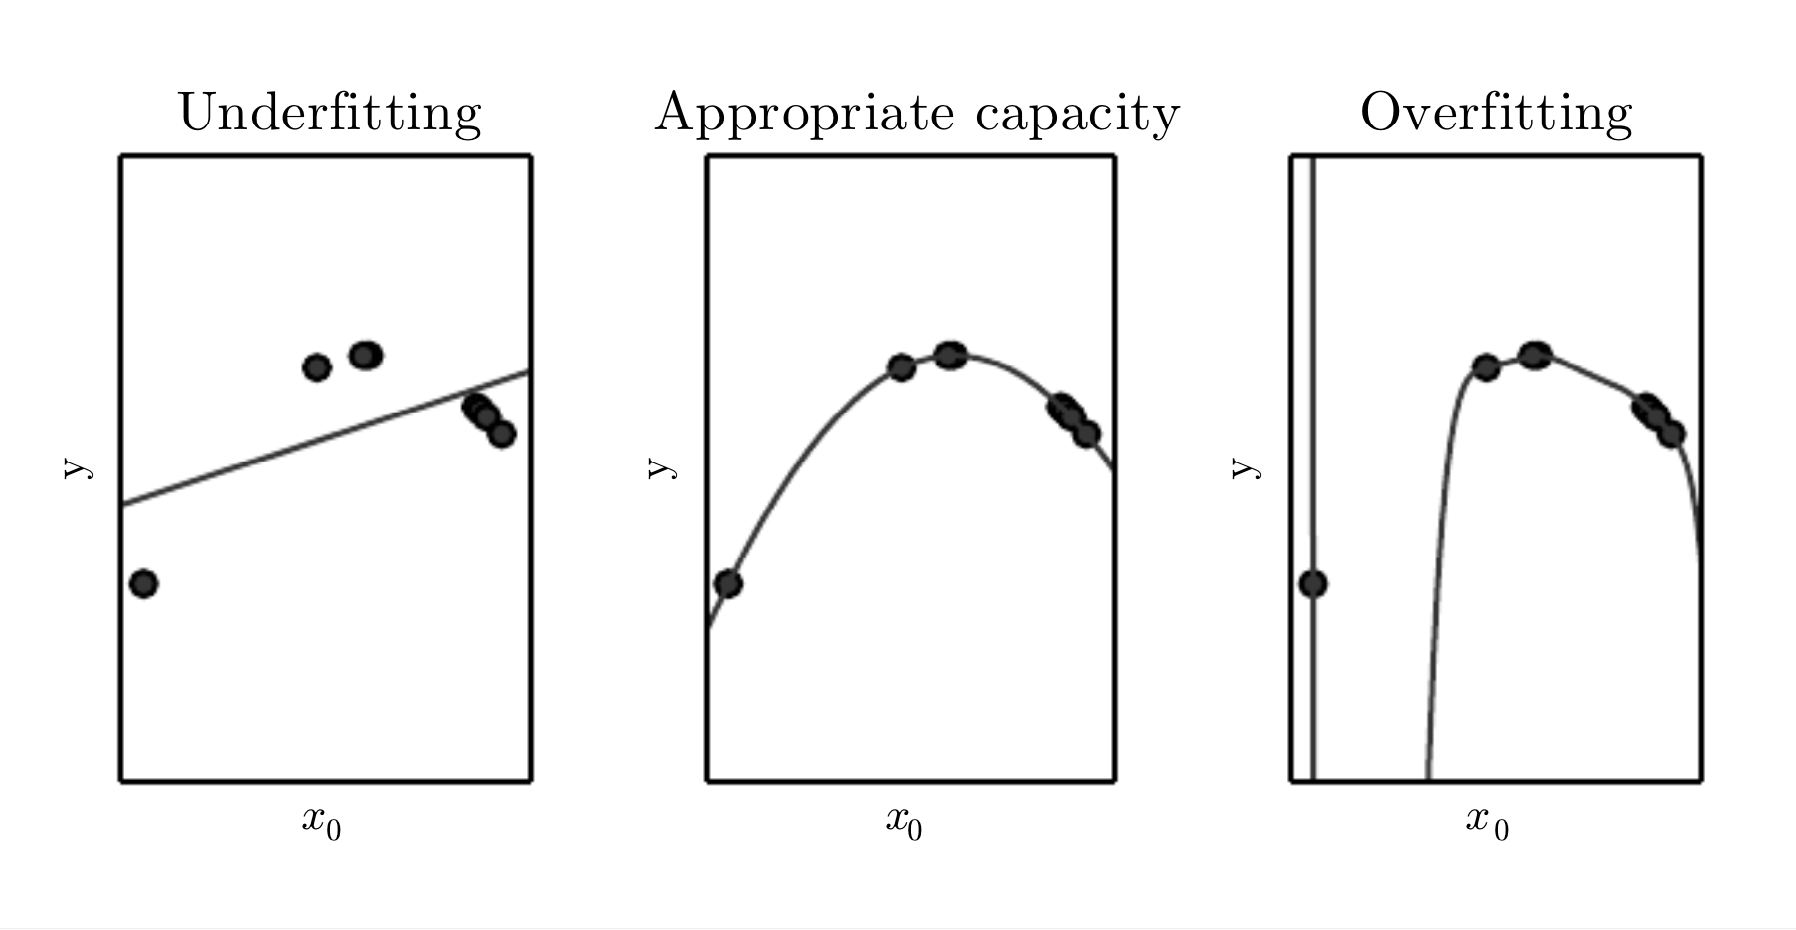
\includegraphics[height=8cm]{img/overfitting}
  \caption[Overfitting, underfitting and appropriate capacity]{Overfitting, underfitting and appropriate capacity~\footcite{Goodfellow2016}}
\label{fig:overfitting}
\end{figure}

\textbf{Overfitting} simply refers to a large gap between training error and test
error.
Intuitively, the model learns too much about specific examples in the training
set and can not perform well on other data.
In contrast to that, \textit{underfitting} occurs when the model is not able
to explain a significant portion of variance in the data.
Fig.~\ref{fig:overfitting} displays examples for both phenomena, as well as
an appropriate model in the context of curve fitting.
Overfitting is often a result of long-running training processes which are
not regularized appropriately.
The following paragraphs describe techniques commonly used to avoid overfitting.

\textbf{Dropout} aims to solve a commonly occurring problem in deep neural networks
called `co-adaption'~\footcite{Hinton2012a}.
It refers to neurons that detect features whose usefulness can not be isolated,
but is dependent on the detection of other features.
Such a neuron is only helpful in conjunction with other neuron.
Co-adaptation can cause overfitting, because it creates an opportunity for
the network to model patterns in the training data in an excessively detailed
way.
Contrary, neurons should learn to detect features that are useful in isolation.
Applying dropout refers to random deactivation of a prespecified percentage
of neurons.
Neurons that are omitted in this way, are removed on the forward pass of an
iteration.
This can be achieved by setting the activations to zero instead of computing
them.
On the backward pass, weights that are connected to deactivated neurons receive
no updates.
The only necessary parameters for each layer using droput is the percentage
of active neurons $p$.
This represents the probability that the neuron is present during training.
When applying the network to test data, all units are present to make predictions.
However, weights from all network layers using dropout are multiplied by $p$.
This makes the application of dropout straighforward.
Despite its algorithmic simplicity, dropout has been shown to reduce overfitting
in several deep architectures~\footcite{Srivastava2014}.

Another, even more recently developed regularization technique is \textbf{batch
normalization}.
It addresses the problem of slowly converging training processes caused by
\textit{internal covariate shift}, which is the amount by which layer activations
change over the course of many iterations.
This amount is influenced by the fact that the distribution of layer activations changes
as the parameters connected to it are updated.
In order to deal with varying activation distributions the learning rate often
has to be lowered which in turn can slow down network training considerably.
Batch normalization addresses this problem by normalizing layer inputs for
a mini-batch of examples in an iteration.
Intuitively, this makes sense since data is often normalized in preprocessing
before being put into a model.
Technically, inputs are normalized along all dimensions $k$ by subtracting the mean
and dividing by the standard deviation of respective dimension (see equation~\ref{eq:bn_norm}).

\begin{align}
  \widehat{x}^{(k)} = \frac{x^{(k)} - E[x^{(k)}]}{\sqrt{Var[x^{(k)}]}} \label{eq:bn_norm} \\
  y^{(k)} = \gamma^{(k)} \widehat{x}^{(k)} + \beta^{(k)} \label{eq:bn_scale_shift}.
\end{align}

Normalizing layer inputs in this way limits internal covariate shift, but also
limits the representational capability of these neurons.
Therefore, batch normalization adds learnable parameters $\gamma$ and $\beta$ for
each input, which serve to scale and shift the input after normalization~\ref{eq:bn_scale_shift}.
Hence, the network can learn to undo the normalization (\textit{denormalization})
if necessary.
Batch normalization has been shown to speed up the training process and also
reduce overfitting which limits the necessity for dropout~\footcite{Ioffe2015}.

\begin{figure}[h]
  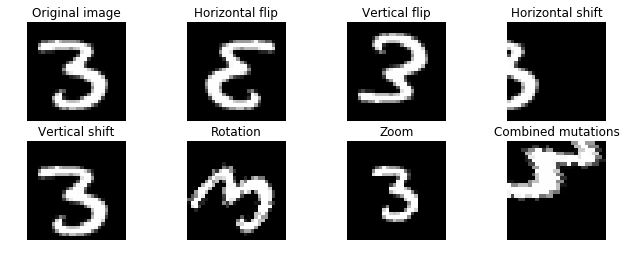
\includegraphics[height=6.5cm]{img/data_augmentation}
  \caption{Self-created examples of augmented images}
\label{fig:augmented_images}
\end{figure}

As described in Chapter~\ref{sub:dl_drivers}, deep neural networks profit from
large amounts of data.
Therefore, the first step in reducing overfitting is usually to add
more data.
This can be achieved using either more real data, or by generating new examples
from already used training data.
This technique called \textbf{data augmentation} is common in computer vision
problems that deal with images~\footcite{Simard2003}.
It refers to the enhancement of training data with variations of existing training
examples.
For images these augmented images can created using minor mutations, e.g., random rotations, flips, shifts or
color changes.
Fig.~\ref{fig:augmented_images} shows examples of a handwritten character being
mutated in various ways.
Data augmentation leads to a bigger variety of inputs, which has been shown
to reduce overfitting for deep neural networks~\footcite{Krizhevsky2012}.


\subsubsection{Practical Applications}
\label{sub:dl_applications}

The previous chapter section covered recent progress in neural network research
on a theoretical level.
After gaining an understanding of modern architectures and training techniques,
this chapter will present practical applications of deep learning.
The upcoming subsections explain problems from multiple areas of computer
science, that can be approached using neural networks.
Namely, sections cover applications in Natural Language Processing (ch.~\ref{sub:dl_app_nlp}),
Computer Vision (ch.~\ref{sub:dl_app_cv}) and Reinforcement Learning (ch.~\ref{sub:dl_app_rl}).

\paragraph{Natural language processing (NLP)}
\label{sub:dl_app_nlp}

Section~\ref{sub:dl_architectures} introduced the problem of \textit{language modeling},
i.e., learning a probability distribution for words in a given sequence.
Convolutional and recurrent neural networks have been successfully applied to
this problem, in many cases improving previous state-of-the-art performance
on benchmark data sets.
Both network architectures are combined within complex models, so that these
so-called \textit{neural language models} are able to encode multiple
languages~\footcite{Kim2015}.
Another application of neural networks lies in the area of \textit{text classification},
i.e., assignment of a given text or document into predefined categories.
An example for this problem is classification of news articles into classes such
as sports, finance or politics.
This is an additional area in which deep learning shows increased performance
over previous approaches, mostly through the use of deep convolutional neural
networks~\footcite{Conneau2016}.
The most recently solved problem in natural language processing is \textit{machine
translation}, which aims to automate conversion of text between different
languages.
Complexity is here derived from the necessity of encoding the source language and
then decoding the learned representation into the target language.
Both model components, i.e., encoder and decoder, have shown to be efficiently
learnable with LSTMs (see ch.~\ref{sub:dl_architectures})~\footcite{Sutskever2014}.
The practical relevance of this research area is exemplified by contributions
from corporate research departments, e.g., \textit{Google}~\footcite{Wu2016}.

\paragraph{Computer vision}
\label{sub:dl_app_cv}

\begin{figure}[h]
  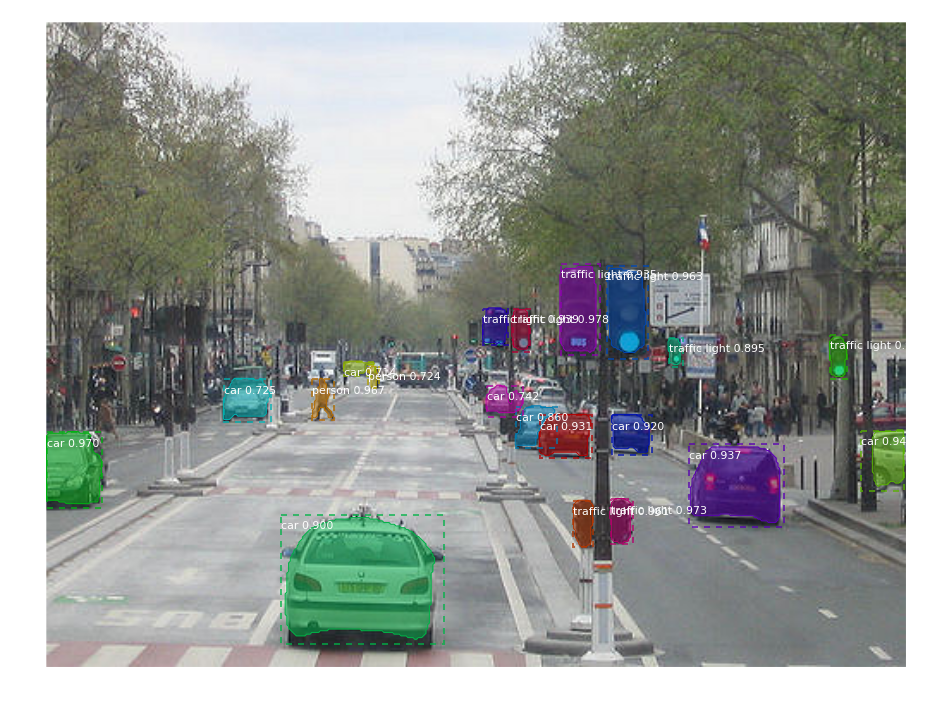
\includegraphics[height=10cm]{img/mask_rcnn}
  \caption[Object detection example]{Object detection example in street scenery~\footnote{\url{https://github.com/matterport/Mask_RCNN}}}
\label{fig:obj_detection}
\end{figure}

The area of computer vision mainly aims to process image and video data in
various ways.
Example problems that are solved using deep learning methods are presented in
the following.
As mentioned in previous chapters, \textit{image recognition} describes the
process of assigning images to categories.
Convolutional neural networks were designed to tackle problems like image
recognition by looking at individual sections of images using filters to
detect common features~\footcite{LeCun1998}.
Progress in deep learning allows training deeper models that contain more
convolutional layers and therefore can learn more complex features.
Thus, deep convolutional networks were able to push the state-of-the-art in image recognition~\footcite{Krizhevsky2012, He2016}.
\textit{Object detection} constitutes a related problem, whose goal is
to find all occasions of a predefined set of objects in an image.
Fig.~\ref{fig:obj_detection} shows an example image from a street scenery
with identified objects such as cars or traffic signals.
Deep learning models applied to object detection usually contain convolutional
layers to identify regions of interest in an image and map these to the
specified object classes~\footcite{Girshick2012, He2017}.
High-performance object detectors can then be used for even more advanced
tasks such as \textit{visual tracking}, i.e., following objects over several video
frames, or \textit{image captioning} which aims to describe images~\footcite{Bertinetto2016, Karpathy2017}.

\begin{figure}[h]
  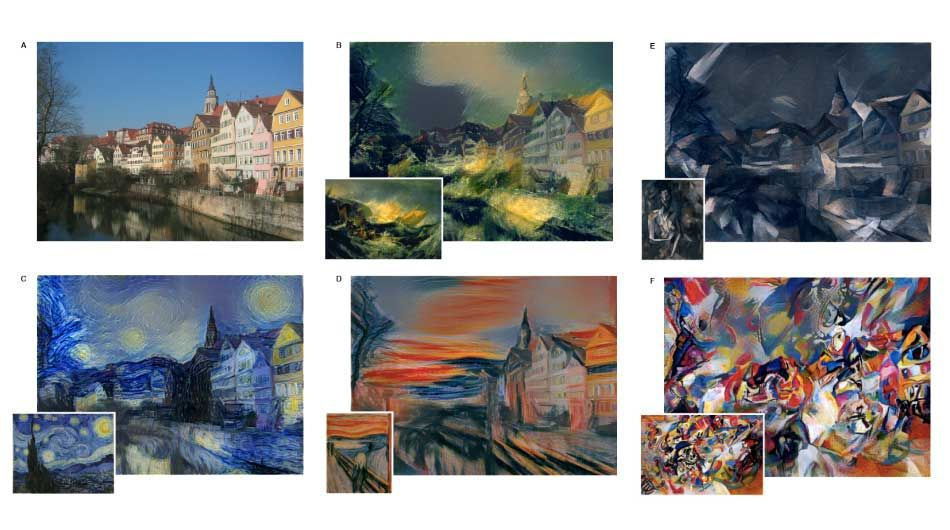
\includegraphics[height=9cm]{img/style_transfer.jpg}
  \caption[Style transfer example]{Style transfer example~\footcite{Gatys2015}}
\label{fig:style_transfer}
\end{figure}

Convolutional neural networks have also been used for generative tasks like
\textit{style transfer}.
Here, the goal is to apply styles of a source image, e.g., texture or colors,
to a target image.
An example is shown in Fig.~\ref{fig:style_transfer}, where a house scenery is
repainted in the style of various artists~\footcite{Gatys2015}.
Related tasks include image generation, where generative adversarial networks
show good performance~\footcite{Radford2015}.
Style transfer and image generation are also examples for unsupervised learning
problems, as introduced in ch.~\ref{sub:dl_terminology}, because there is
generally no labeled data for these tasks.

\paragraph{Reinforcement learning}
\label{sub:dl_app_rl}

Reinforcement learning constitutes another kind of experience for machine
learning algorithms.
In this setting, an agent continuously interacts with its environment and learns
from feedback in the form of rewards.
In order to estimate rewards for specific actions, the current state of the
given setting has to be evaluated.
Deep learning models have mostly been applied to evaluate settings that can
be displayed visually.
For example, this is the case for video games where each video frame represents an image.
Convolutional neural networks are used to detect patterns in the current
setting which are helpful for an agent and its decision about upcoming
actions.
Recently, researchers were able to train agents that perform better than human
professionals in several games, including simple \textit{Atari} video games
and more complex games like \textit{Go}~\footcite{Mnih2015, Silver2016}.

This chapter concludes the covered deep learning theory for this thesis.
The upcoming chapter explains basic concepts of social networks in general and
\textit{Twitter} more specifically, which are necessary for understanding
upcoming experiments.


\subsection{Social Networks}
\label{sec:social_networks}

Applying deep learning to tweet engagement prediction requires a basic
understanding of social network dynamics and structure. Furthermore, a common
understanding of Twitter terminology is necessary for later chapters of this
work. Both areas will be covered in this section, beginning with social
networks in general (ch.~\ref{sub:sn_terminology}) and concluding with
Twitter in detail (ch.~\ref{sub:sn_twitter}).

\subsubsection{Terminology}
\label{sub:sn_terminology}

As with deep learning, social network terminology is sometimes used in confusing
ways.
This subsection aims to eliminate terminology confusion and introduce basic concepts regarding social networks,
as well as related notions like social media.
Firstly, the term \textit{social network} is defined (ch.~\ref{sub:sn_social_networks}), before structural
properties are explained (ch.~\ref{sub:sn_structure} and~\ref{sub:sn_properties}).
The last paragraph of this section focuses on \textit{social media}, especially
practical implications for organizations (ch.~\ref{sub:sn_social_media}).

\paragraph{Social networks}
\label{sub:sn_social_networks}

In order to examine social network structure and properties, the term first
has to be defined.
Wassermann \& Faust (1994) explicate that ``a social network consists of a finite
set or sets of actors and the relation or relations defined on them''~\footcite[20]{Wasserman1994}.
Here, an \textit{actor} can be any social entity, e.g, people, groups, countries or
organizations.
\textit{Relations} are then batches of ties between these entities, e.g., resource
transfers, associations or interactions~\footcite{Wasserman1994}.
With this basic definition set, the next two paragraphs focus on structure and
properties of social networks.

\paragraph{Structure}
\label{sub:sn_structure}

Social networks can be visualized using graphs, where actors serve as nodes
and lines represent relations between these actors.
Thus, the network consists of a set of nodes $N = \{n_1, n_2, \cdots, n_g\}$ and
a set of lines $L = \{l_1, l_2, \cdots, l_L\}$~\footcite{Wasserman1994}.

\begin{figure}[h]
  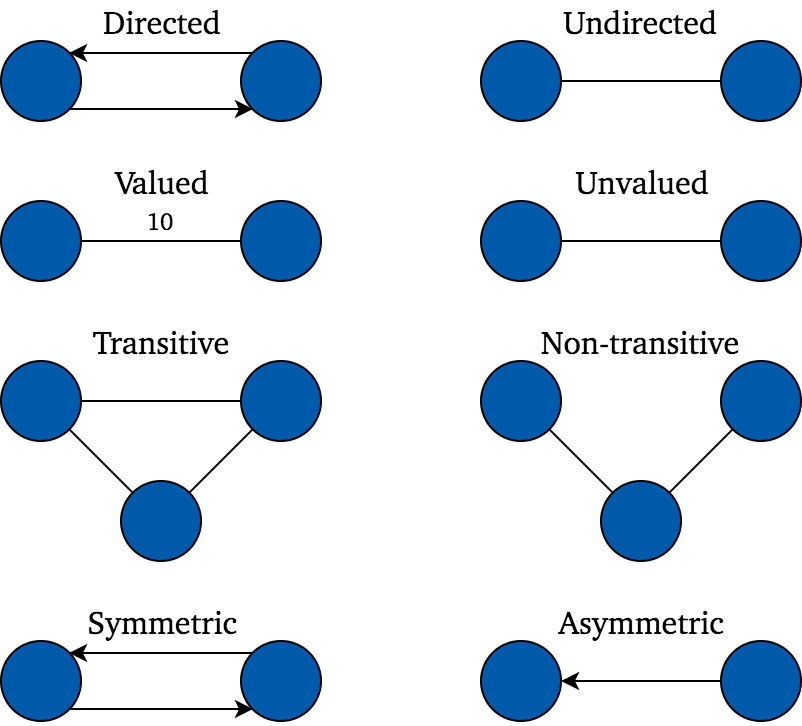
\includegraphics[height=8cm]{img/relation_properties}
  \caption{Relation properties in social networks}
\label{fig:tie_properties}
\end{figure}

Relations between actors can have several properties, as denoted in Fig.~\ref{fig:tie_properties}.
A first distinction has to be made between directed and undirected relations,
a property that also determines the directionality of the underlying graph.
An example for a directed relation would be resource transfers, an undirected
relation could be exemplified by marital relationships.
Relations can also be split into valued and unvalued types.
The attached value can stand for several properties, e.g., interaction intensity
between two actors.
Transitive relations occur when actor triples are connected to each other.
More intuitively, transitivity means that two related actors of an actor $n$ are
also related.
The final property exemplified in Fig.~\ref{fig:tie_properties} is symmetry which
is always given in undirected networks.
For directed networks, symmetry refers to the existence of a relation from
$n_i$ to $n_j$, if there is a relation in the opposite direction~\footcite{Wasserman1994}.

\paragraph{Properties}
\label{sub:sn_properties}

Social network analysis is a research area which examines dynamics in social
networks.
A central research question is the identification of important actors within
a network.
Important actors are also referred to as prestigious or prominent, where importance
represents the extent to which these actors are involved with others.
Here, involvement means being the sender or recipient of interactions in the
network.
A common measure for actor prominence is \textit{centrality}, which delivers
several characteristic numbers for measuring activity and location of an actor~\footcite{Wasserman1994}.
An important observation in social network research is the \textit{small world problem},
which is related to the probability of two random actors in a network being
connected to each other.
Formulated differently, the problem also comprises the question how many
mutual acquaintances are needed to form a path between these random actors.
Experiments lead to the conclusion that the distance between two actors in
a network is surprisingly low~\footcite{Travers1969}.
This gives way to observations that stress the importance of so-called
\textit{weak ties}, i.e., relations between actors that are less intense and
intimate, but serve significant roles in information diffusion~\footcite{Granovetter1973}.

\begin{figure}[h]
  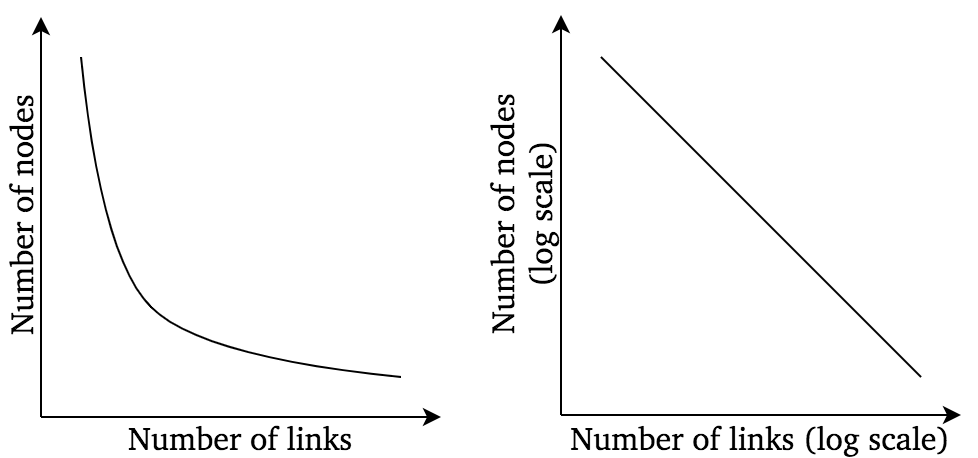
\includegraphics[height=6cm]{img/power_law_linkages}
  \caption[Power Law Distribution of Node Linkages]{Power Law Distribution of Node Linkages~\footcite{Barabasi2003}}
\label{fig:power_law}
\end{figure}

In addition to the small world phenomenon, many social networks are observed to
be \textit{scale-free}.
Scale freedom denotes the observation that few actors have a very high number of connections,
while the vast majority of actors is limited to very few connections.
Highly connected nodes are referred to as \textit{hubs}.
A power law distribution can be observed in scale-free networks, i.e., the
probability for an actor to have exactly $k$ connections is given by $k^{-n}$
where $n$ is approximately 2~\footcite{Barabasi2003}.
Fig.~\ref{fig:power_law} shows the power law distribution of node linkages both
on a regular and log-scale.

\paragraph{Social media}
\label{sub:sn_social_media}

The terms social network and social media are often used interchangeably, though
they generally refer to distinct matters.
Social media can be described as ``a group of Internet-based applications that
build on the ideological and technological foundations of Web 2.0, and that allow
the creation and exchange of User Generated Content''~\footcite[61]{Kaplan2010}.
Here, Web 2.0 refers to technologies like \textit{Flash}, \textit{RSS} and 
\textit{AJAX} that first enabled collaboration on the internet, e.g., via blogs
or wiki pages.
Examples for social media platforms are \textit{Facebook} (social network), 
\textit{Twitter} (microblogging) or \textit{YouTube} (video platform).
Rise of social media platforms brings practical challenges for organizations with it,
since they enable both direct communication with the customer, as well as
communication between customers.
Contents and frequency of the latter are mostly out of managerial control~\footcite{Mangold2009}.
Nowadays, most companies maintain social media profiles as part of their overall
marketing approach.
Research has created guidelines for corporate use of social media and stressed the
importance of community building around products of a company~\footcite{Culnan2010}.
Here, tracking the return of social media investments often requires engagement
statistics, e.g., number of followers, visits or replies, as well as community
sentiment~\footcite{Hoffman2010}.
Attributes of social media marketing have been shown to have positive effects
on purchase intention, e.g., for luxury fashion brands~\footcite{Kim2012}.

Twitter has been listed as an example social media platform.
The concluding section of this background chapter will explain terminology
and properties related to Twitter in more detail.


\subsubsection{Twitter}
\label{sub:sn_twitter}

Twitter is a microblogging service that enables its users to share short
messages with their followers.
The company was founded in 2006 and has grown to 330 million monthly active
users worldwide as of 2017.
Main revenue source for Twitter are advertisements which account for more than
85\% of revenue in 2017.
The last fiscal quarter of 2017 marked the first profitable period in Twitter
history, with profits equalling 91 million USD at a revenue of 732 million USD.
Here, video is the main advertisement format used on the platform~\footcite{Twitter2018}.
Twitter has also invested in live streaming events, e.g., football games~\footnote{\url{https://www.bloomberg.com/news/articles/2016-04-05/twitter-said-to-win-nfl-deal-for-thursday-night-streaming-rights}}.

Later parts of this thesis relate to specific Twitter terminology.
The most common terms will be presented in the following.
Users of the Twitter platform open an account with a unique user name (starting
with the ``@'' symbol).
Users can be verified by Twitter if their account is of public interest, e.g.,
for celebrities, companies or politicians~\footnote{\url{https://help.twitter.com/de/managing-your-account/about-twitter-verified-accounts}}.
If a user wants to receive updates from another user, he can follow his
account.
Relations between users are not necessarily symmetric, resulting in a distinction
between incoming and outgoing links.
Incoming relations,
i.e., being followed, are called ``followers'' and outgoing relations, i.e.,
following, are refered to as ``friends''.
Twitter allows curating users onto lists, which for example enables receiving topic-bound
status updates.
The number of lists a user is assigned to can be found in his account under the
term ``listings''.
Users publish short messages called ``tweets'', which can be seen in their user
account and appear in the timeline of followers.
Other users can engage with tweets through ``favorites'', ``retweets'' and ``replies''.
When sharing a tweet via a retweet, users have the option to add extra content.
If they opt for this approach, the resulting update is treated like a whole new
status message and referred to as a ``quote''~\footcite{Kwak2010}.
Quotes receive distinct engagement statistics, whereas engagement in retweets
is counted towards the original message.
The above described differentiation is important for later parts of this thesis.

This section about Twitter terminology completes the background chapter.
The next chapter will explain the general methodology used in this work.


\chapter{Methodology}
\label{ch:methodology}

Having established necessary background knowledge in the previous chapter,
the experiments of this work can be introduced.
This chapter will first examine prior work in the area of tweet engagement
prediction (ch.~\ref{sec:prior_work}), before outlining limitations of this
research.
Afterwards, structure and aim of the developed models will be explained in general (ch.~\ref{sec:approach}).
The final section of this section describes the data sets used in this work,
as well as the collection process (ch.~\ref{sec:data_collection}).

\outline{Add infrastructure section}

\section{Prior Work}
\label{sec:prior_work}

This section lists previous work in tweet engagement prediction, starting with
general retweet research and then introducing models that cope with different
kinds of prediction problems.
Predictive models in this area are largely focused on retweet prediction.
This can be explained by the sharing effect of retweeting, which can be interpreted
as information diffusion, a highly researched area in social network analysis.
Previously developed models were roughly classified according to their problem type.

\paragraph{General retweet research}

General research on the act of retweeting offers intuitions about the mechanism
and gives way for feature ideas for machine learning models.
Boyd et al.~\cite{Golder} examine conversational aspects of retweeting and
compare the mechanism to other behavioral conventions on the Twitter platform,
namely mentions and hashtags.
Where mentions constitute a form of direct messaging and hashtags enable
communication around specific topics, retweeting is a form of information
diffusion and participating in conversations without actively contributing.
Furthermore, the authors identify motivations for retweeting, e.g., showing
presence as a listener or validating a tweet.
According to their examination, the most commonly retweeted content is
time-sensitive, e.g., breaking news.
Factors influencing retweetability have also been the subject of other work.
Features are often separated into content and contextual features.
Among content features, the use of URLs and hashtags has been shown to be
positively correlated with retweetability, especially for URLs that are seen
as particularly interesting by human respondents~\cite{Suh}.
Contextual features comprise all factors related to the source user, his
following and activitiy on the platform.
The number of followers and friends, as well as account age have positive
effects on retweetability.
Moreover, past activity, e.g., tweet frequency was shown to not be significantly
influential~\cite{Bakshy2011, Suh}.
Retweeting has also been analyzed in temporal fashion, mainly through the use
retweet graphs which constitute representations of cascades.
Kwak et al.~\cite{Kwak2010} show that most retweeting acts occur in the first
and second degree network of the source user.
Additionally, most retweeting happens in a concise time frame.
Namely, 50 \% of retweets take place within one hour, 75 \% within a day and more
than 90 \% in one month after tweet creation.

\paragraph{Retweet probability prediction}

Retweet probability prediction refers to the problem of forecasting the
probability that a given destination user will retweet a specific tweet of
the source user.
This problem has drawn interest from the research community in the past, and
multiple models have been developed for this purpose.
First models only used very simple features like tweet words, identity of the
source user and the number of his followers and friends~\cite{Zaman2010}.
Other work focuses on content features, which can be divided into two separate
categories.
Low-level features include used words, the number of hashtags, URLs and mentions,
as well as usage of positive and negative terms according to predefined word 
classification.
High-level features on the other hand describe more complex features such as
the association to topics or sentiments.
Naveed et al.~\cite{Naveed2011} develop a logistic regression model using
both types of features and find that tweets regarding more general and 
negatively connoted topics have a higher probability of being retweeted.
More complex features are included by Peng et al.~\cite{Peng2011},
who employ conditional random fields for their predictive model.
The authors include content features such as topic similarity of a tweet with 
interests of the source user and his audience.
In addition, activity data is used, e.g., tweet frequencies of user and
followers around specific times.
A new set of features involves the relationship between source and destination
user, i.e., the number of mutual followers, friends and mentions.
It is shown that user features are most helpful for the prediction of
retweet probability.
Lee et al.~\cite{Lee2014} go a step further and try to identify the most
effective message propagator for a given tweet.
They rely on a rich set of manually crafted features around personality and activity data
and employ different machine learning models, e.g., random forest, logistic
regression and support vector machines.

\paragraph{Classification approaches}

As introduced in ch.~\ref{sub:dl_terminology}, classification models learn a
mapping between inputs and predefined sets of outputs.
A model employing an output variable with exactly two possible values is referred
to as a \textit{binary classification model}.
This approach can be used for retweet prediction approach, namely if the goal
of the model is to simply determine whether a given tweet will be retweeted
or not.
So-called \textit{multi-class classification models} aim to deliver a more
precise prediction regarding the number of retweets.
Hong et al.~\cite{Hong2011} have developed both types of models in their work
using a logistic regression approach.
Whereas the binary classification model shows promising results, the multi-class
model only performs well for predicting retweet counts of 0 and larger than
10,000.
Classes inbetween these two extremes are predicted with much lower accuracy.
Another binary classification model was introduced by Petrovic et al.~\cite{Petrovic2011}
who focus on the creation a deployable model.
This leads to the utilization of simple content and contextual features, as described
in the above paragraph.
They find that contextual features, especially regarding the source user,
have higher predictive power than tweet features.
The models achieve accuracy metrics between 70 and 80 \% on different tasks,
which is not significantly different from recorded human performance.

\paragraph{Regression approaches}

Regression models aim to predict a specific value for given inputs.
For retweet prediction this refers to forecasting a numerical value for the
eventual retweet count.
Since the retweet process after tweet creation has no preset determination date, general assumptions
about the temporal retweet distribution have to be made when building
regression models.
Kupavskii et al.~\cite{Kupavskii2012} try to predict the eventual size of the
retweet cascade, i.e., the graph whose vertices represent retweeting users.
At the time, this constituted a novel task which enables two distinct predictions:
one at the initial point of tweet creation, the second after a short
time of observing the retweet cascade.
Obviously, the second prediction can be made using more information about the
initial message spread.
The authors employ a gradient boosted decision tree based on standard content
features (see above paragraphs).
Additionally, they take retweet ratios of creating user and followers into
account and precalculate PageRank statistics for all considered users on a
separate data set of retweet graphs.
Thus, they gain more insights into retweeting behavior of users in their data
set.
As expected, observing retweet cascades for some time improves the quality
of their prediction considerably.
A comparable approach is used by Zaman et al.~\cite{Zaman2014}, whose work
examines retweet time series for 52 manually chosen tweets.
They find that the median of all retweets occurs between four minutes and three
hours after tweet creation.
In addition, they develop a Bayesian model for evaluating the retweet graph
which is able to utilize parts of the time series data to improve its
prediction.
The model outperforms a linear regression baseline using only
the follower count as input data.
Moreover, the prediction becomes more precise the more time series data is utilized
as an input.

Having established this line of prior research, the approaches used in this
work can now be described.


\subsection{Approach}
\label{sec:approach}

The introduction to this thesis stated its main objective, namely the
development of a deployable stand-alone model for precisely predicting tweet
engagement metrics.
As previously elaborated, `deployable' in this context stands for the practical
applicability of the model.
The term `stand-alone' denotes the requirement of solely relying
on data that stems directly from tweet objects of the public Twitter interface.
Not being dependent on additional data would enable the system to be applicable
in a streaming setting.
Furthermore, predicted engagement metrics should incorporate both eventual
retweet and favorite counts.
This section comprises three parts.
Firstly, limitations of the previously described prior work with regard to the
stated objective are outlined.
Secondly, the experiments conducted in this thesis are introduced.
Finally, necessary assumptions for the developed models are stated and justified.

\subsubsection{Limitations of prior research}

This thesis aims to develop deep learning models for predicting tweet
engagement.
Employing deep learning should help to overcome several limitations of prior
work in this research area (see ch.~\ref{sub:meth_prior_work}), which will be listed in the following.
Some of the described models rely on complex, manually crafted features, e.g.,
activity, topic similarity and relationship features.
These often require additional data and excessive preprocessing, in some cases
even precalculated models on separate data sets.
This stands in contrast to the ad-hoc processing requirement in the objective.
The hypothesis of this work is that these features can be omitted or
learned intrinsically by deep neural networks.
Manual feature creation is necessary for machine learning models like logistic
regression or decision trees that are less capable of creating own feature
representations.
Deep neural networks achieve higher representational capability by effectively
stacking non-linear modules which learn discrete features according to the problem at
hand~\cite{LeCun2015}.
One objective for this thesis is an accurate prediction of the eventual popularity
of tweets.
Previous models mostly focus on probability prediction or binary classification
which is insufficient to meet this objective.
Furthermore, less complex models have not shown good performance in the multi-class
classification setting, only showing good accuracy for extreme cases.
This work tries to overcome this limitation by employing deep models on diverse
data sets with varying class distributions.
Following this approach should also conquer biases in the collected data.
In previous research, data sets were often collected around a single topic or
trend, sometimes even handpicked~\cite{Zaman2014}.
Both models that apply predictive models in a regression setting are dependent
on some form of time-series observation of the retweet graph, which is not adequate for
an accurate prediction about future engagement at the time of tweet creation.
In this work, models are able to make real-time predictions, i.e., it could
be possible to deploy them in an application that is fed data from the Twitter
Streaming API~\footnote{\url{https://developer.twitter.com/en/docs/tweets/filter-realtime/overview/powertrack-api}}.
An additional feature of models in this work is their capability to predict both
number of retweets and favorites.

\subsubsection{Developed models}

Models developed in this thesis make use of content and contextual features,
inspired by previous work in this field.
Since the models only rely on tweet objects from the Twitter API, contextual
features are mainly limited to information about the source user~\footnote{\url{https://developer.twitter.com/en/docs/tweets/data-dictionary/overview/intro-to-tweet-json}}.
In contrast to previous model, sophisticated deep learning models should allow
more precise processing of tweet content, particularly because deep neural networks
show good performance on natural language processing tasks (see ch.~\ref{sub:dl_app_nlp}).
In summary, the deep models are fed both structured and unstructured data.
Here, structured data represents inputs that could easily be stored in
tabular format, e.g., a relational database.
Examples for these features include number of hashtags and URLs on the content
side, as well as follower count and account age on the contextual side.
The actual tweet content can be seen as unstructured data, due to its variation
in length and manifestation.

\begin{figure}[h]
  \centering
  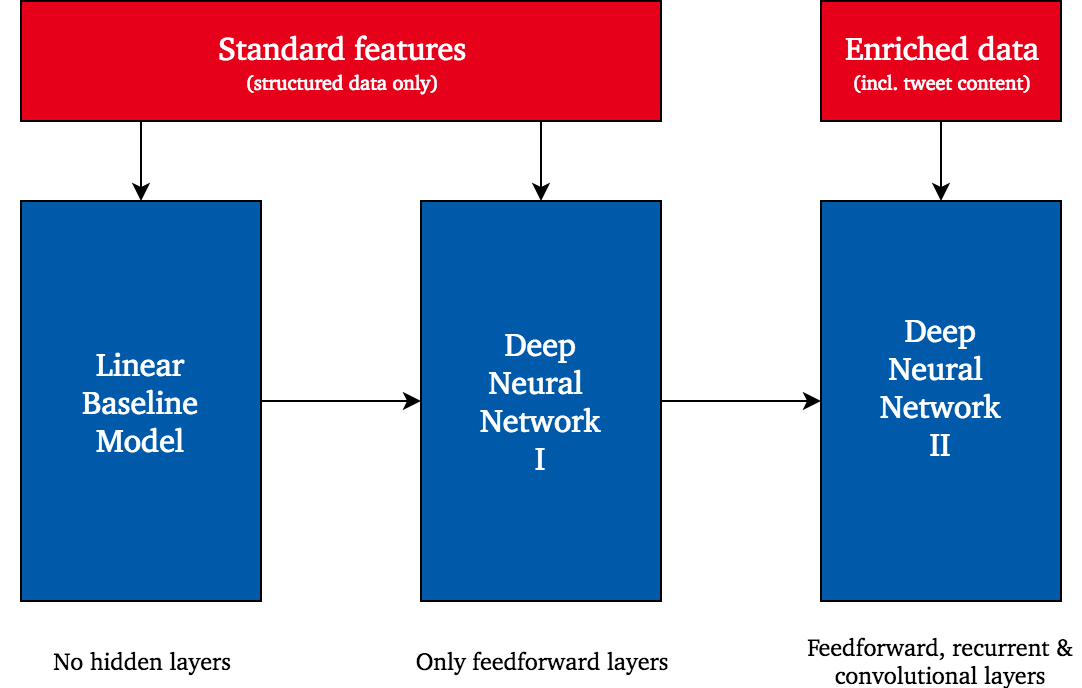
\includegraphics[height=9cm]{img/model_summary}
  \caption{Summary of developed models}
\label{fig:model_summary}
\end{figure}

Fig.~\ref{fig:model_summary} sums up the intended model evolution for this thesis.
Each model will be used in both a regression and multi-class classification
setting, producing separate predictions for retweet and favorite counts.
In order to enable comparisons, a linear baseline model will be created first.
This model will be trained solely using structured data.
In their essence, these models represent linear and logistic regression models
respectively.
Afterwards, a deep neural network is trained on the same structured data sets.
This model employs standard feed-forward layers (see ch.~\ref{sub:dl_concepts}),
which enables more complex input representations and hence more accurate
predictive outputs.
The final model is trained using enriched, i.e., structured and unstructured,
input data and more sophisticated layer architectures.
Both convolutional and recurrent layers are deployed in order to derive more
powerful features from the tweet content. 
Including textual input data requires additional preprocessing steps which aim
to transform words into floating-point numbers.
However, these additional steps do not hinder the practical applicability
of the model since they are not costly computation-wise.

\subsubsection{Assumptions}

This work relies on the assumption that most retweeting occurs in a short time
span after tweet creation.
Following this assumption, retweet and favorite counts can be approximated
to be precise estimates of the tweet engagement one month after the initial
creation.
This important assumption can be justified by research which conducts analysis
on large tweet data sets.
The overall conclusion of such research is that half of retweeting occurs within
hours, and more than 90 \% within one month after tweet publication~\cite{Kwak2010, Kupavskii2012, Zaman2014}.

Having established intended experiments for this work, the concluding section
in this methodology chapter will describe the examined data sets and the
collection process.


\subsection{Data}
\label{sec:data_collection}

The main goal of this thesis regarding the examined data is to have diverse
data sets from users for which engagement prediction has practical relevance.
The diversity requirement mainly comprises different retweet distributions
so that the model performance can evaluated in a generalized manner.
Predicting the popularity of tweets is relevant for all individuals and
organizations that somehow rely on social media marketing or customer support.
Therefore, the collected data sets include data from public figures and
companies, most of whom actively maintain a Twitter account.
The selected accounts were separated into three groups and saved as Twitter lists
in the author's profile (see Appendix).
For each of the three groups, all tweets from January to August 2017 were
fetched from the public Twitter API~\footnote{\url{https://developer.twitter.com/en/docs/tweets/timelines/api-reference/get-statuses-user_timeline.html}}.
Afterwards, retweets that the specified users made were excluded since their
engagement statistics are not related to their accounts, but the users who
originally created their tweets.
In summary, the final data sets include all status updates and quotes from the
specified users in the given time frame.
It was ensured that all collected tweets were older than one month 
at the time of retrieval.
As mentioned in the previous section, the third stage of model development
for this thesis aims to extract meaningful features from the raw tweet content.
This typically requires a huge number of data points, so that popular NLP benchmark
data set for similar tasks, e.g., sentiment analysis, usually contain more than
a million labeled training examples~\footcite{Go2009}.
In order to account for these massive data requirements, an additional data set was
collected, which includes all tweets from the aforementioned user groups over
the course of two years.

\begin{table}
\begin{tabular}{lllr}
\toprule
  Accounts & Total accounts & Time frame & Total tweets \\
\midrule
  Fortune 500 companies & 441 & 1/2017 - 8/2017 & 254,059 \\
  US Governors and Senators & 162 & 1/2017 -  8/2017 & 94,919 \\
  Celebrities & 170 & 1/2017 - 8/2017 & 46,986 \\
  Companies, politicians \& celebrities & 773 & 1/2016 - 12/2017 & 863,004 \\
\bottomrule
\end{tabular}
\caption{Summary of collected data sets}
\label{tab:dataset_summary}
\end{table}

Table~\ref{tab:dataset_summary} sums up all data sets used for the purpose of
this work.
The first data set comprises all Twitter accounts from \textit{Fortune 500}
companies in 2017~\footnote{\url{http://fortune.com/fortune500/}}.
All in all, 441 out of 500 companies operate a Twitter presence, which accounted
for a total of 254,059 tweets in the evaluated period.
The second user group includes all Twitter accounts of US Senators~\footnote{\url{https://twitter.com/cspan/lists/senators}} and Governors~\footnote{\url{https://twitter.com/cspan/lists/governors}}
as of October 2017 which were derived from Twitter lists by the television
network \textit{C-SPAN}.
From January to August 2017, 162 politicians created a total of 94,919 tweets.
The smallest data set stems from celebrities, namely the \textit{Forbes Highest-Paid
Athletes 2017}~\footnote{\url{https://www.forbes.com/sites/kurtbadenhausen/2017/06/15/full-list-the-worlds-highest-paid-athletes-2017}}, \textit{Forbes Highest-Paid Actors and Actresses 2017}~\footnote{\url{https://www.forbes.com/sites/natalierobehmed/2017/08/22/full-list-the-worlds-highest-paid-actors-and-actresses-2017}} and
\textit{Forbes Highest-Paid Celebrities 2017}~\footnote{\url{https://www.forbes.com/sites/zackomalleygreenburg/2017/06/12/full-list-the-worlds-highest-paid-celebrities-2017}}.
The derived data set contains 46,986 tweets from 170 accounts.
Over the course of 2016 and 2017, all users combined accounted for a total
of 863,004 tweets which comprise the additional data set.
It has to be mentioned that company tweets account for an unproportionally high
percentage (around 60\%) of all tweets in this data sets, simply due to greater
total of accounts from this group.

Examining deep neural network performance on differently sized data sets should
enable to draw conclusion about data requirements for the particular problem
of engagement prediction.
Descriptive statistics for all data sets can be found in ch.~\ref{sec:dda}.


\subsection{Infrastructure}
\label{sec:infrastructure}

The experiments in this thesis were conducted using infrastructure suitable
to handle complex computations and large data sets.
This section will describe hardware (ch.~\ref{sub:meth_hardware}) and software
(ch.~\ref{sub:meth_software }) which was applied to the problem of tweet
engagement prediction.

\subsubsection{Hardware}
\label{sub:meth_hardware}

As stated in Chapter~\ref{sub:dl_drivers}, training deep neural networks
typically requires the parallel computing power of graphics processors.
In addition, large data files need to be stored and processed.
Cloud environments are well suited for these tasks, since they enable on-demand 
access to specialized hardware.
\textit{Amazon Web Services} was chosen as primary infrastructure provider for 
work on this thesis, mainly due to familiarity and a broad palette of offered
solutions.
Raw, unfiltered data files containing tweet and author information were stored
on an \textit{Amazon S3}\footnote{\url{https://aws.amazon.com/s3/}} instance,
which could be accessed programmatically or via the management console.
After filtering retweets and extracting features, the prepared data sets could
permanently be saved on the respective processing instance for improved
accessibility.
Training of deep learning models was undertaken on an \textit{Amazon EC2}\footnote{\url{https://aws.amazon.com/ec2/}}
instance.
Namely, the specification \textit{p2.xlarge} was chosen in order to train models
on a GPU.
These instances employ a \textit{NVIDIA K80} GPU with 12GB of memory and 2,496
processing cores.
Moreover, p2.xlarge machines possess 61GB of memory and four CPU cores.

\subsubsection{Software}
\label{sub:meth_software}

All model development was conducted using the \textit{Python}\footnote{\url{https://www.python.org/}} programming language,
since it offers extensive and well-docomented libraries for data analysis and numerical computation.
\textit{Jupyter notebooks}\footnote{\url{http://jupyter.org/}} were used as development environment, because
of their capability to combine code, visualizations and documentation in a single
document.
Conducting experiments in notebooks proved to increase reproducibility of results
and overall project organization.
Reusable functionality tested in notebooks was often transferred to Python
modules.

\outline{Development environment: Jupyter notebooks (+ self-written Python modules)}

\outline{Data collection: python-twitter library}
\outline{Possible alternatives: using API directly, wrangling with JSON (not as convenient)}

\outline{Data analysis and wrangling: pandas, numpy, matplotlib, scikit-learn}

\outline{Model training: Keras (high-level API) with Theano backend (low-level: cudNN, CUDA)}
\outline{Possible alternatives: TensorFlow, PyTorch (not as familiar to author)}

This section about infrastructure concludes the methodology chapter.
The upcoming chapter will describe results of experiments undertaken in this
thesis.


\section{Results}
\label{ch:results}

This chapter will outline results of experiments conducted for this thesis,
according to the methodology outlined in the previous chapter.
Firstly, Chapter~\ref{sec:dda} delivers explorative analysis of all three
collected data sets, comparing them along several dimensions.
Afterwards, the developed models will be introduced along with an evaluation
of their predictive performance.
Included features, model architectures, necessary preprocessing steps and results will
be described for linear baseline (ch.~\ref{sec:linear_models}),
deep feedforward (ch.~\ref{sec:deep1}) and more complex deep models
(ch.~\ref{sec:deep_combined}).

\subsection{Descriptive Data Analysis}
\label{sec:dda}

Developing machine learning models for predicting certain outcomes requires
an understanding of the underlying data.
Insights derived from descriptive data analysis are useful in all steps of the
modeling process, e.g., for preprocessing, feature extraction and evaluation
of model performance.
For this thesis, exploratory data analysis also serves the purpose of establishing
differences between the three examined data sets.
The upcoming sections compare the collected data sets along the dimensions of
engagement metrics (ch.~\ref{sec:engagement_stats}), network characteristics
(ch.~\ref{sec:network_stats}) and general account activity (ch.~\ref{sec:activity_stats}).
Prior to presenting the results of this analysis, a few remarks about presentation
have to be made.
In almost all cases, data is discretized to improve clarity.
Here, all created bins, e.g., in histograms, are left-inclusive and right-exclusive.
For example, the bin `1-10k' denotes all observations between 1,000 and
9,999 (for a variable scaled as an integer).
In addition, all represented distributions are normalized to account for varying
data set sizes and improve comparability.

\subsubsection{Engagement statistics}
\label{sec:engagement_stats}

Examining engagement statistics for all three data sets is crucial since the goal
of this thesis is to predict these variables.
This section will therefore compare retweet and favorite distribution for 
celebrity, politician and corporate tweets.

\begin{table}
\centering
\begin{tabular}{lrrr}
\toprule
Retweets & Celebrities & Politicians & Companies \\
\midrule
Mean & 1,629.8 & 318.4 & 15.1 \\
Median & 176.0 & 23.0 & 1.0 \\
\midrule
Favorites & Celebrities & Politicians & Companies \\
\midrule
Mean & 6,135.6 & 832.9 & 40.3 \\
Median & 1117.0 & 69.0 & 1.0 \\
\midrule
Pearson correlation & Celebrities & Politicians & Companies \\
\midrule
Correlation coefficient & 0.9188 & 0.9457 & 0.9803 \\
\bottomrule
\end{tabular}
\caption{Summary of engagement statistics}
\label{tab:engagement_summary}
\end{table}

Table~\ref{tab:engagement_summary} indicates that celebrity tweets are engaged
with most often.
This holds true when looking at central tendency statistics (mean and median)
for retweet and favorite counts.
Moreover, in this sample politician tweets are more popular compared to tweets from corporate
accounts.
For all three data sets, strong correlation between the number of favorites and retweets can
be stated.
This observation is useful for later model development, because it can be concluded that
both variables should be predictable using similar statistical models, e.g.,
a multi-output model with differently scaled weights in the last layer.
The differences between mean and median values point to skewness in the
underlying distributions.
Since the calculated means are significantly larger than their respective
median values, observations should extend farther to the right
of the distributions.
This finding can be explained twofold. 
Firstly, retweet and favorite counts have an obvious  minimum of zero.
Secondly, a small number of very popular tweets constitute outliers which largely
influence the mean calculation.
In order to examine engagement distributions in more detail, Fig.~\ref{fig:retw_distr} and
Fig.~\ref{fig:fav_distr} illustrate engagement statistics which are discretized into logarithmic bins (base 10).
Above discretization also corresponds to the classes used for the classification models
of this thesis.

\begin{figure}[h]
\centering
\begin{subfigure}{.33\textwidth}
  \centering
  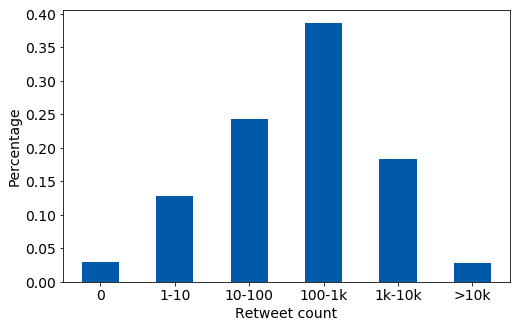
\includegraphics[width=.95\linewidth]{img/celeb_retw_distr}
  \caption{Celebrity data set}
  \label{fig:retw_distr_sub1}
\end{subfigure}%
\begin{subfigure}{.33\textwidth}
  \centering
  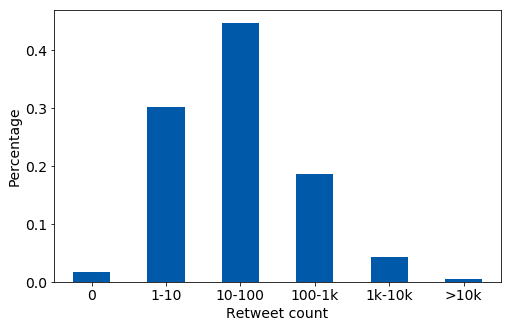
\includegraphics[width=.95\linewidth]{img/polit_retw_distr}
  \caption{Politician data set}
  \label{fig:retw_distr_sub2}
\end{subfigure}
\begin{subfigure}{.33\textwidth}
  \centering
  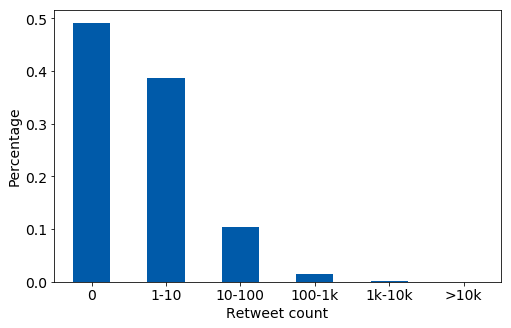
\includegraphics[width=.95\linewidth]{img/corp_retw_distr}
  \caption{Company data set}
  \label{fig:retw_distr_sub3}
\end{subfigure}%
\caption{Retweet distributions}
\label{fig:retw_distr}
\end{figure}

\begin{figure}[h]
\centering
\begin{subfigure}{.33\textwidth}
  \centering
  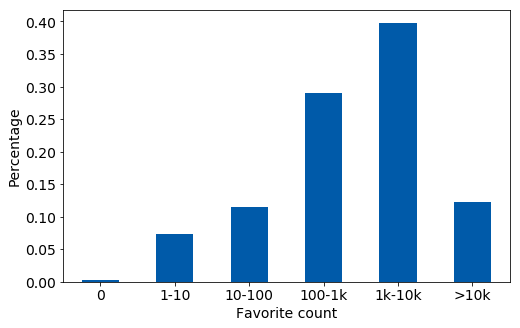
\includegraphics[width=.95\linewidth]{img/celeb_fav_distr}
  \caption{Celebrity data set}
  \label{fig:fav_distr_sub1}
\end{subfigure}%
\begin{subfigure}{.33\textwidth}
  \centering
  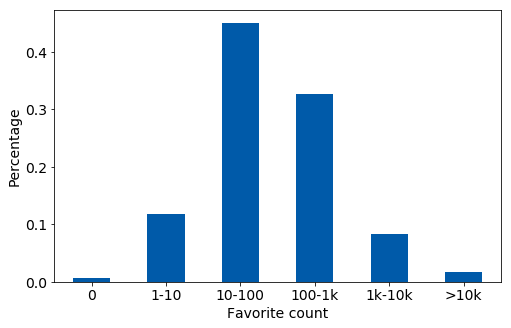
\includegraphics[width=.95\linewidth]{img/polit_fav_distr}
  \caption{Politician data set}
  \label{fig:fav_distr_sub2}
\end{subfigure}
\begin{subfigure}{.33\textwidth}
  \centering
  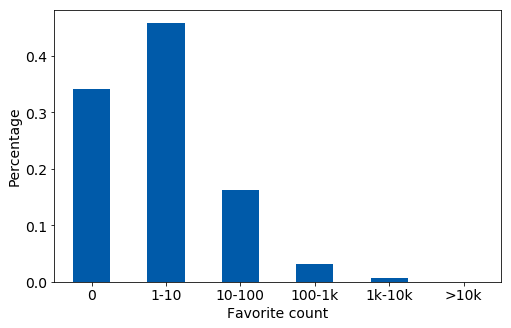
\includegraphics[width=.95\linewidth]{img/corp_fav_distr}
  \caption{Company data set}
  \label{fig:fav_distr_sub3}
\end{subfigure}%
\caption{Favorite distributions}
\label{fig:fav_distr}
\end{figure}

All three data sets possess class imbalance, i.e., some classes are more likely
to occur than others.
Here, differences in class probabilities are significant across data sets
and variables, with the most common class
containing close to or more than 40\% of all observations and some classes
hardly being represented at all.
Looking at retweets it can be stated that celebrity and politician distributions
have a Gaussian-like shape, where the central tendency of celebrity tweets is
farther to the right.
Company retweet classes seem to be more exponentially shaped.
Moving to favorites, central tendencies of all distributions are clearly pushed to the right of the
spectrum, which accounts for the generally observed difference between favorite
and retweet counts.

The upcoming subsections further describe characteristics of the collected
data sets and provide possible explanations of the found discrepancies in
retweet and favorite distributions.

\subsubsection{Network statistics}
\label{sec:network_stats}

Prior work in this area suggests the importance of user data when predicting
popularity of created tweets.
The most obvious features in this category are the number of incoming and outgoing
connections, i.e., follower and friend counts in the context of Twitter.
This section shows the distribution of these variables in the previously
defined user groups and examines the correlation with engagement metrics.

\begin{table}
\centering
\begin{tabular}{lrrr}
\toprule
Number of followers & Celebrities & Politicians & Companies \\
\midrule
Mean & 10,255,423 & 331,944 & 357,023 \\
Median & 3,228,642 & 89,072 & 23,204 \\
Correlation w/ retweets & 0.1457 & 0.2828 & 0.0326 \\
Correlation w/ favorites & 0.1922 & 0.3423 & 0.0442 \\
\midrule
Number of friends & Celebrities & Politicians & Companies \\
\midrule
Mean & 5,587 & 3,775 & 5,513 \\
Median & 241 & 599 & 800 \\
Correlation w/ retweets & 0.1799 & 0.0030 & -0.0036 \\
Correlation w/ favorites & 0.1754 & 0.0092 & -0.0049 \\
\bottomrule
\end{tabular}
\caption{Summary of network statistics}
\label{tab:network_summary}
\end{table}

\begin{figure}[h]
\centering
\begin{subfigure}{.33\textwidth}
  \centering
  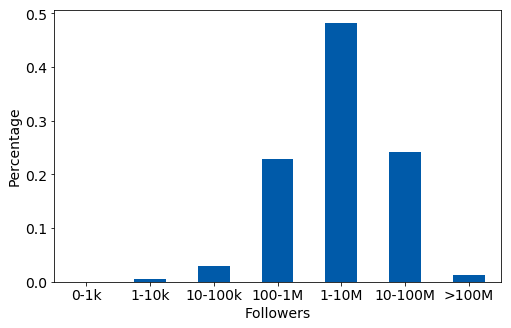
\includegraphics[width=.95\linewidth]{img/celeb_follow_distr}
  \caption{Celebrity data set}
  \label{fig:follow_distr_sub1}
\end{subfigure}%
\begin{subfigure}{.33\textwidth}
  \centering
  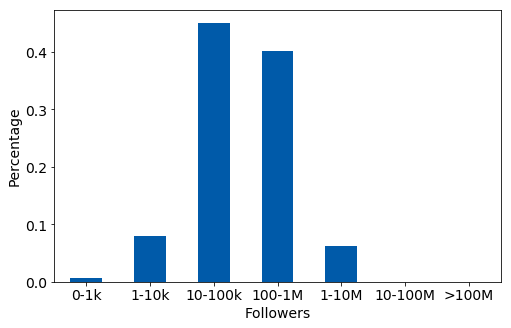
\includegraphics[width=.95\linewidth]{img/polit_follow_distr}
  \caption{Politician data set}
  \label{fig:follow_distr_sub2}
\end{subfigure}
\begin{subfigure}{.33\textwidth}
  \centering
  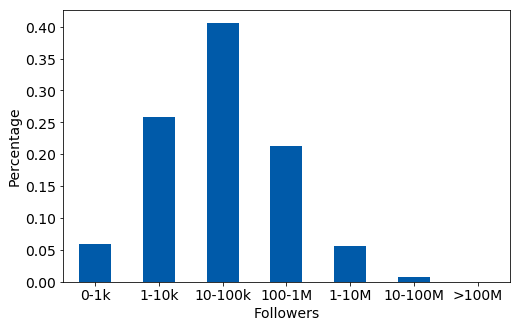
\includegraphics[width=.95\linewidth]{img/corp_follow_distr}
  \caption{Company data set}
  \label{fig:follow_distr_sub3}
\end{subfigure}%
\caption{Follower distributions}
\label{fig:follow_distr}
\end{figure}

Table~\ref{tab:network_summary} summarizes network statistics for all three
user groups.
It can be stated that celebrities tend to have the largest following on average,
followed by companies and politicians.
Most celebrities are followed by more than a million accounts, whereas the
majority of politicans and companies have followings smaller than 100 thousand
accounts (see Fig.~\ref{fig:follow_distr}).
Again, follower and friend distributions are skewed to the right across all
groups.
Considering the previously demonstrated differences in retweet and favorite
distributions, one could assume a correlation between number of followers
and tweet popularity.
However, linear correlation with retweet and favorites counts is nonexistent
(celebrities and companies) or only weakly positive (politicians).
Correlation coefficients are even lower for the number of friends a user
possesses.
The friend distributions have a similar shape, more than half of all users
follow less than 1,000 accounts (see Fig.~\ref{fig:friend_distr}).
The median value is highest for corporate accounts which seems logical, since
these accounts are probably most often managed using more manpower.
Particularly strong linear relationships between number of friends and engagement statistics can not
be found.

\begin{figure}[h]
\centering
\begin{subfigure}{.33\textwidth}
  \centering
  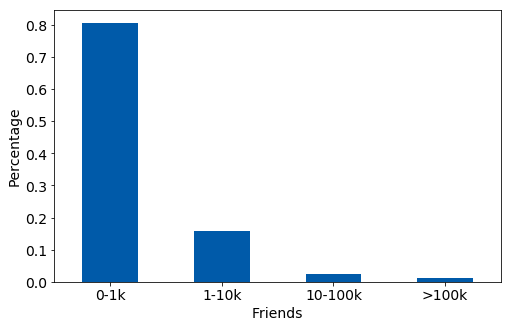
\includegraphics[width=.95\linewidth]{img/celeb_friend_distr}
  \caption{Celebrity data set}
  \label{fig:friend_distr_sub1}
\end{subfigure}%
\begin{subfigure}{.33\textwidth}
  \centering
  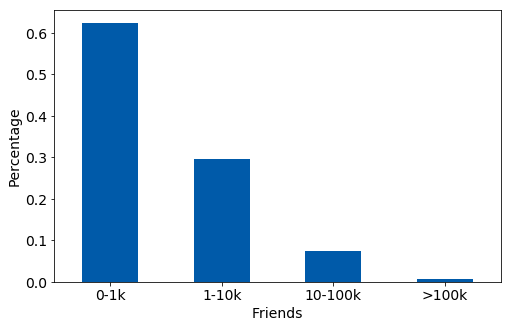
\includegraphics[width=.95\linewidth]{img/polit_friend_distr}
  \caption{Politician data set}
  \label{fig:friend_distr_sub2}
\end{subfigure}
\begin{subfigure}{.33\textwidth}
  \centering
  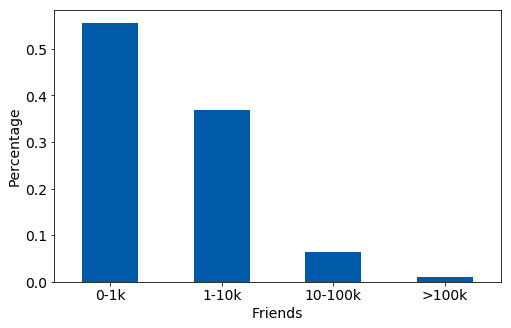
\includegraphics[width=.95\linewidth]{img/corp_friend_distr}
  \caption{Company data set}
  \label{fig:friend_distr_sub3}
\end{subfigure}%
\caption{Friend distributions}
\label{fig:friend_distr}
\end{figure}

\subsubsection{Activity statistics}
\label{sec:activity_stats}

Like network data, activity statistics have been used as features in previously
developed models which serve the purpose of retweet prediction.
Both feature groups can be classified in the category of contextual features,
as opposed to content features.
This section will describe account age and tweet frequency as indicators
for user activity.

\begin{figure}[h]
\centering
\begin{subfigure}{.33\textwidth}
  \centering
  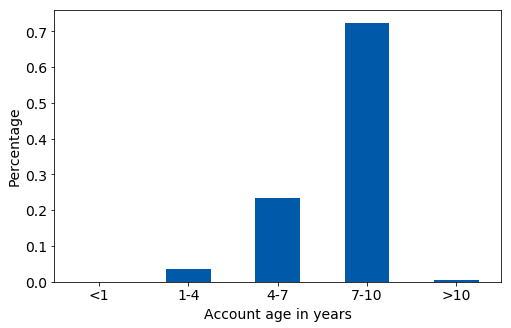
\includegraphics[width=.95\linewidth]{img/celeb_age_distr}
  \caption{Celebrity data set}
  \label{fig:age_distr_sub1}
\end{subfigure}%
\begin{subfigure}{.33\textwidth}
  \centering
  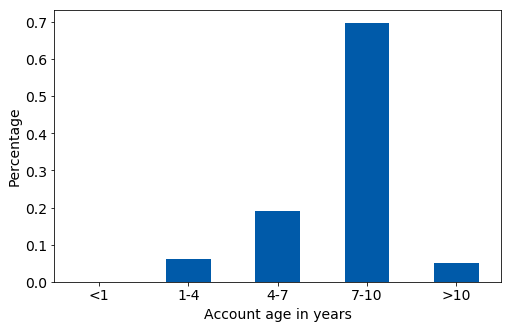
\includegraphics[width=.95\linewidth]{img/polit_age_distr}
  \caption{Politician data set}
  \label{fig:age_distr_sub2}
\end{subfigure}
\begin{subfigure}{.33\textwidth}
  \centering
  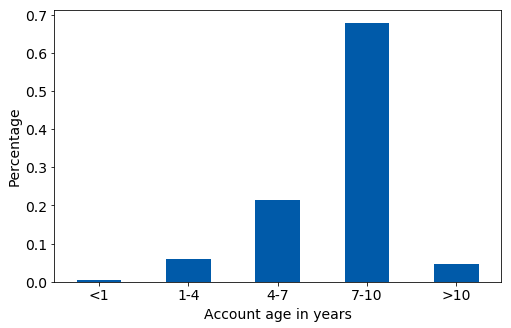
\includegraphics[width=.95\linewidth]{img/corp_age_distr}
  \caption{Company data set}
  \label{fig:age_distr_sub3}
\end{subfigure}%
\caption{Account age distributions}
\label{fig:age_distr}
\end{figure}

Fig.~\ref{fig:age_distr} shows the account age distributions, calculated for
each user group individually.
Superficially, the distributions look similar.
For all groups, around 70\% of all accounts are seven to ten years old, thus being
created two to four years after Twitter was opened for public access.
Earlier adopters mainly stems from the politician and company user groups, about
5\% of accounts in these groups are older than ten years.
There is hardly any skewness in the account age distribution, i.e., median and
mean values are close to each other.

\begin{figure}[h]
\centering
\begin{subfigure}{.33\textwidth}
  \centering
  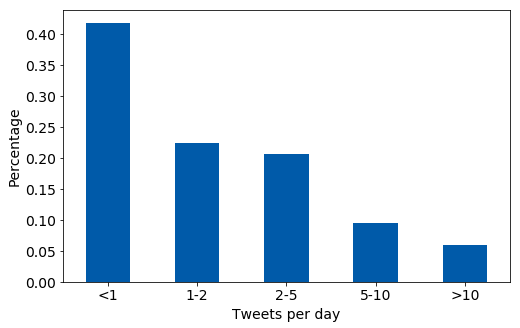
\includegraphics[width=.95\linewidth]{img/celeb_freq_distr}
  \caption{Celebrity data set}
  \label{fig:freq_distr_sub1}
\end{subfigure}%
\begin{subfigure}{.33\textwidth}
  \centering
  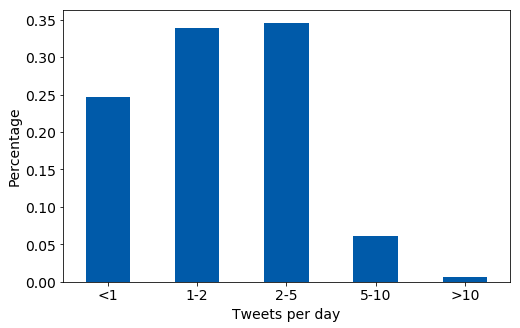
\includegraphics[width=.95\linewidth]{img/polit_freq_distr}
  \caption{Politician data set}
  \label{fig:freq_distr_sub2}
\end{subfigure}
\begin{subfigure}{.33\textwidth}
  \centering
  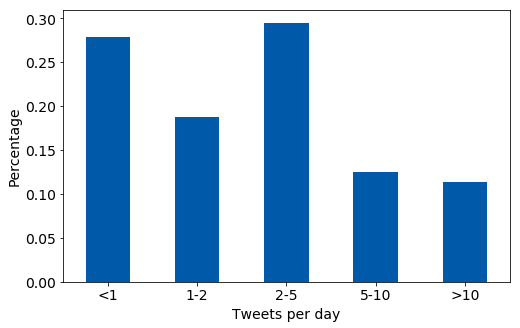
\includegraphics[width=.95\linewidth]{img/corp_freq_distr}
  \caption{Company data set}
  \label{fig:freq_distr_sub3}
\end{subfigure}%
\caption{Tweet frequency distributions}
\label{fig:freq_distr}
\end{figure}

Although accounts exemplify rougly the same age distribution across all user
groups, their activity level differ considerably (see Fig.~\ref{fig:freq_distr}).
Many celebrities do not average one tweet per day and the median for this group (1.20)
is lower than the respective counterparts for politicians and companies (1.75 resp. 2.16).
However, these numbers are not surprising, since many companies user their accounts
for daily customer support.
This could also explain the high percentage of accounts with more than ten tweets
per day in this group (so-called \textit{power users}).
It can also be stated that users from the politician user group tend to concentrate
in the range of under five tweets per day.
The 75th percentile is the lowest for all three user groups (2.83 tweets per day).
Neither account age nor tweet frequency show any direct linear correlation with
retweet or favorite counts for the collected tweets.
In more detail, all correlation coefficients are located between -0.1 and 0.1 (all
calculated values can be found in the appendix of this thesis).

This section concludes the descriptive data analysis part of this thesis.
Observations derived from these analyses are used in subsequent sections,
particularly for feature extraction and performance evaluation.


\section{Linear Models}
\label{sec:linear_models}

This section comprises results of linear engagement prediction models that
were trained as a baseline for later comparison with deep neural networks.
This kind of model evolution allows analysis of performance improvements
with regard to standardized metrics.
As is the case for all models, both multi-class classification and regression
models were developed for all three data sets.
This section starts with describing the model architecture (ch.~\ref{sub:lin_architecture}) and continues by detailling the training process (ch.~\ref{sub:lin_training}).
It concludes by summarizing results and analyzing model performance in more detail
(ch.~\ref{sub:lin_performance}).

\subsection{Model architecture}
\label{sub:lin_architecture}

\begin{figure}[h]
  \centering
  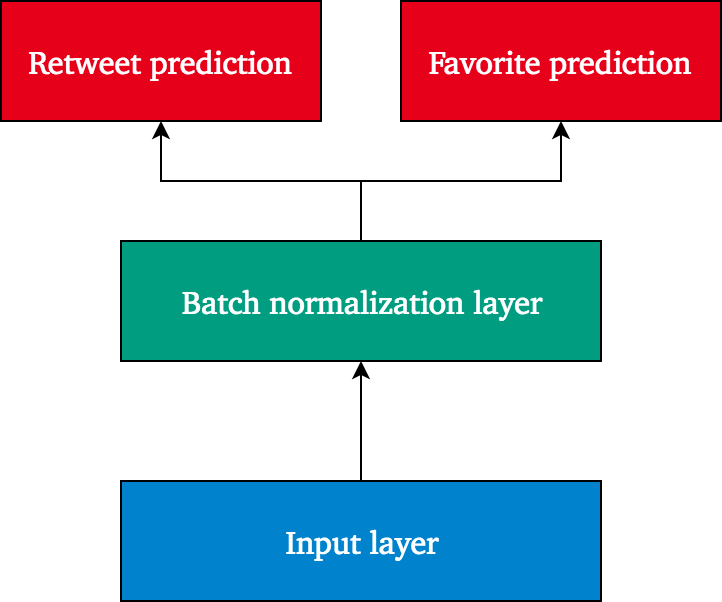
\includegraphics[height=8cm]{img/linear_model_architecture}
  \caption{General architecture of linear models}
\label{fig:linear_model_architecture}
\end{figure}

Fig.~\ref{fig:linear_model_architecture} illustrates the general architecture
of linear models trained in this work.
Firstly, inputs are normalized using a \textit{batch normalization} (see ch.~\ref{sub:dl_regularization})
layer in order to account for different scaling in the features.
As stated before, this layer type allows the model to undo normalization at
training time if it serves the purpose of better output representation.
The normalized inputs are then directly mapped onto two distinct outputs,
one for the number of retweets and one for the number of favorites.
In this case, regression and classification models only differ in their
respective type of prediction.
The regression model simply outputs two numbers representing retweet and
favorite estimates.
Hence, this constitutes a \textit{linear regression model}, because the output is not transformed.
Contrary, the classification model should output class probabilities for each
of the six predefined classes (see Table~\ref{tab:classification_buckets}).
As a result, the outputs have to be split according to the number of classes and transformed
using the \textit{sigmoid function} (see ch.~\ref{sub:dl_forward}).
This kind of model is called \textit{logistic regression} and is considered
a linear classifier despite the outputs being transformed using a non-linear
function.
The reason for that is the sole reliance on a linear combination of the
(normalized) inputs.

\begin{table}
\centering
\begin{tabular}{ll}
\toprule
Feature & Description \\
\midrule
URL count & Number of URLs \\
Hashtag count & Number of hashtags \\
Mention count & Number of mentioned users \\
Tweet length & Length in characters \\
Quoted tweet & Is tweet a quote? \\
\midrule
Follower count & Number of followers the tweet author has \\
Friend count & Number of friends the tweet author has \\
Verified status & Is the tweet author verified? \\
User listings & Number of lists tweet author was added to \\
User tweet count & Total number of tweets by tweet author \\
User overall tweet frequency & Tweets per day by tweet author \\
User favorite count & Total number of given favorites by tweet author \\
User overall favorite frequency & Number of given favorites per day by tweet author \\
User account age & Number of days since account creation \\
Hour of tweet creation & Hour of the day the tweet was created \\
\bottomrule
\end{tabular}
\caption{Linear model features}
\label{tab:structured_features}
\end{table}

All input features (see Table~\ref{tab:structured_features}) are directly derived
from collected tweet objects.
Since these objects contain information about the tweet author, no further data lookups
are necessary.
Consequently, these features can be extracted with minimal preprocessing, which
enables model application in a real-time prediction setting.
The structured inputs are separated into content (top half) and contextual
features (bottom half).
Activity statistics, i.e. frequencies, are calculated on a per-day basis,
the hour of tweet creation is given in \textit{Coordinated Universal Time (UTC)}.
The previouly described need for normalization becomes obvious, e.g., when
comparing scales for URL counts (usually 0-3) and account age (thousands of days).
Content features mainly incorporate information on the use of conversational
tools (URLs, mentions, hashtags), but do not model the tweet content itself.
In addition, contextual features comprise popularity and activity information
about the tweet author.

\begin{table}
\centering
  \begin{tabular}{lr}
    \toprule
    Class & Range \\
    \midrule
    1 & 0 \\
    2 & 1-9 \\
    3 & 10-99 \\
    4 & 100-999 \\
    5 & 1,000-9,999 \\
    6 & >10,000 \\
    \bottomrule
  \end{tabular}
  \caption{Classes for classification models}
  \label{tab:classification_buckets}
\end{table}

General model output types were previously described.
In short, regression models output a positive real-valued estimate of the
eventual favorite and retweet count.
Classification models on the other hand aim to predict the probability that
these counts are within a certain range.
The prefined ranges represent the output classes and are shown in Table~\ref{tab:classification_buckets}.
Basically, the classes represent a logarithmic scale of eventual engagement counts.
Since retweet and favorite counts are wide-ranging in all three data sets,
scaling the outputs logarithmically creates a more balanced class distribution.
As described in section~\ref{sec:engagement_stats} the underlying class distributions
are still far from uniform.
However, the data sets proved to be large enough to learn this slightly 
imbalaced distribution with more complex models (see subsequent sections).
Other common methods for handling class imbalance, e.g., penalizing misclassifications
in rare classes via class weights, did not improve results significantly.
Retweet and favorite prediction are treated equally, i.e., the final loss
is calculated by building the mean of loss values for the singular tasks.

After establishing model architecture including input and output types, the next
session will explain details about the training process.

\subsection{Training process}
\label{sub:lin_training}

Accurate model comparisons require a standardized setting regarding training
processes.
Therefore, the following paragraphs will describe important aspects of model training
used in this work.
In particular, data usage, training duration and choices of optimization
algorithm and cost functions will be explained and motivated.

Prior to training, all three data sets were split into training and validation
data according to a 90\%/10\% split.
Since the splitting process was undertaken after permutating the example order
randomly, class distributions in training and validation sets should be very
similar.
Training examples were used to learn the weights of the model, whereas validation
examples are not known to the algorithm during training.
Consequently, the unseen data could be used to derive an estimate of the model
generalizability.
Models were trained for a fix number of iterations, each iteration consisting
of a full pass over all training examples.
Here, training data was split into batches of 128 examples whose gradients
were averaged in order to derive weight updates.
Testing was conducted to determine the required number of iterations for
convergence in loss function minimization.
The regression models turned out to converge slower, so that these models
had to be trained for a longer period of time.
In summary, regression models were trained for 150 iterations, whereas classification
models already converged after 50 iterations.

After comparing multiple optimization algorithms on data samples, \textit{adaptive
moment estimation (Adam)} was used for all experiments in this work.
Recapping from ch.~\ref{sub:dl_optimization_algos}, this recently developed
algorithm adapts learning rates for each parameter based on mean and variance of
recent updates.
It therefore combines strengths of previously developed techniques such as
\textit{momentum} and \textit{RMSprop}.
Tests showed faster convergence and more stability of the training process, i.e.,
fewer iterations were needed to derive an acceptable minimum of the loss function.
The default parameters detailed in the background chapter turned out to be sufficient
for linear models and did not require adjustments.

\textit{Adam} was applied to the minimization of two different cost functions for
classification and regression models.
Mathematical formulas and reasoning behind the choice of both functions
is outlined in the following.

\begin{equation}
  \label{eq:cross_entropy}
  C = -\frac{1}{n} \sum_x \sum_j y_j \ln a_j^L + (1 - y_j) \ln (1 - a_j^L)
\end{equation}

Evaluating performance of a classification model is mainly based on the ability
of the model to classify examples correctly.
Hence, the derived probability for the correct class should be close to one and
in that case, the value of the cost function for this example should be close
to zero (since cost functions are by definition minimized).
Equation~\ref{eq:cross_entropy} illustrates the \textit{categorical cross-entropy}
cost function. Here, $a_j^L$ represents the output of the last layer $L$ for class $j$,
evaluated on example $x$.
Intuitively, this is the probability estimate for example $x$ belonging to class $j$.
Cross-entropy calculates the natural logarithm of this estimate and multiplies
it with the desired output $y$, which is one if $x$ belongs to this class and
zero otherwise.
Thus, the cost for this example is derived from the first summand of the equation
if the example actually belongs to this class.
In the contrary case, the second summand determines the cost.
For both terms it holds, that the higher the difference between estimate and desired
output, the higher the value of the cost function will be (since the equation is negated).
The final cost for one example is derived by summing over all classes.
In order to calculate the loss value for one batch, the costs of all examples
in the batch are averaged.
Cross-entropy has come to be a standard cost function for classification
models, because it relies on probabilities and not just boolean values for class
membership.
Therefore, it allows more precise performance evaluation.
However, the metric is not interpretable directly.
Accordingly, results in this work will also list the metric \textit{accuracy}, which simply
denotes the percentage of correctly classified examples.
Results tables will abbreviate these metrics as \textit{CCE} and \textit{Acc}
respectively.

\begin{equation}
  \label{eq:mae}
  C = \frac{1}{n} \sum_x |y - a^L|
\end{equation}

A more directly interpretable cost function can be chosen for regression models.
Experiments in this work were conducted using \textit{Mean Absolute Error (MAE)},
which constitutes the average deviation between actual and desired outputs
in a batch of examples (see Equation~\ref{eq:mae}).
Interpretability was one of the reasons for choosing this metric over another popular alternative,
\textit{Root Mean Squared Error (RMSE)}.
Both metrics express an average prediction error in the respective variable unit,
here number of retweets or favorites.
However, MAE is more directly interpretable because output values
are not transformed at all and there is no distinction between error magnitudes.
By squaring error terms, RMSE penalizes large errors unproportionally higher
than small errors.
This is not desirable for the use case of this work, where underlying
engagement distributions come from a broad range of possible values.
\textit{Mean absolute percentage error (MAPE)} would have obvious benefits
on such a wide-ranging distribution, but it is not applicable in the existence
of zero values (which are present in all data sets).

\subsection{Model performance}
\label{sub:lin_performance}

After creating a standard setting for experiments across all data sets, 
results of training the linear models will be presented in this section.
Firstly, a summary of general performance metrics will be given, before
evaluating the classification models in more detail.
Finally, possible interpretations detected results will be listed.

\begin{table}
\centering
  \begin{tabular}{lrrrrrrr}
    \toprule
    & \multicolumn{4}{l}{Classification} & \multicolumn{3}{l}{Regression} \\
    \midrule
    Data set & CCE & Acc & Ret Acc & Fav Acc & MAE & Ret MAE & Fav MAE \\
    \midrule
    Celebrities & 1.22 & 48.84\% & 47.15\% & 50.52\% & 3,490.21 & 1,552.63 & 5,427.79 \\
    Politicians & 1.04 & 54.17\% & 51.64\% & 56.70\% & 482.81 & 273.83 & 691.80 \\
    Companies & 0.95 & 59.64\% & 63.38\% & 55.90\% & 24.66 & 13.02 & 36.29 \\
    \bottomrule
  \end{tabular}
  \caption{Summary of linear model results}
  \label{tab:lin_model_results}
\end{table}

Table~\ref{tab:lin_model_results} summarizes linear model results for all three
data sets.
For the classification task, both categorical cross-entropy (CCE) and
accuracy (Acc) metrics are given, regression performance is measured using
mean absolute error (MAE).
In addition, more detailed information about performance on the singular tasks of
retweet and favorite prediction is listed for the more interpretable metrics.
Data sets are staged in order of increasing data set size.
It can be generally observed that model performance improves with data set size, i.e.,
accuracy increases and loss values decrease.
For example, class predictions are 10\% more accurate for the company data set
than for celebrity tweets.
Moreover, retweet class predictions are more accurate than favorite class predictions
for celebrity and politician tweets.
Opposite behavior can be observed for the company data set.
For regression models, learning retweet prediction yields better results than
the counterpart task of predicting favorite counts.
However, this has to be expected since retweet counts are considerably smaller
and thus more narrowly distributed than favorites.
A wider underlying distribution of engagement counts, i.e., larger mean and median values, might also be the reason
for higher estimation discrepancies on celebrity and politician data.
In general, the observed results are not compelling for both classification and
regression models and leave room for improvements using deep neural networks.

\begin{figure}[h]
\centering
\begin{subfigure}{.5\textwidth}
  \centering
  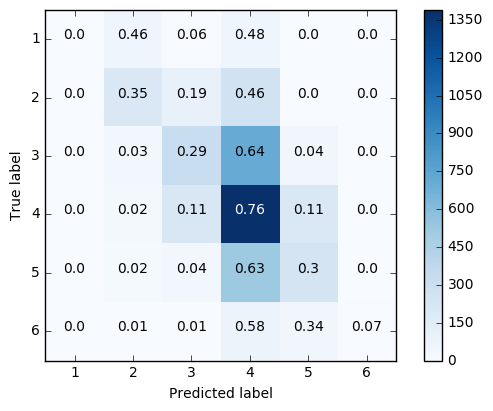
\includegraphics[width=.95\linewidth]{img/celeb_lin_cm_retweets}
  \caption{Celebrity data set}
  \label{fig:retw_distr_sub1}
\end{subfigure}%
\begin{subfigure}{.5\textwidth}
  \centering
  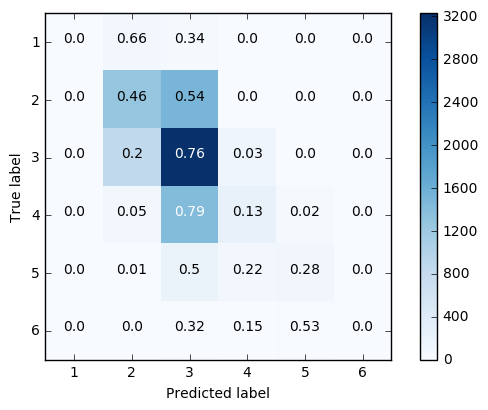
\includegraphics[width=.95\linewidth]{img/polit_lin_cm_retweets}
  \caption{Politician data set}
  \label{fig:retw_distr_sub2}
\end{subfigure}
\begin{subfigure}{.5\textwidth}
  \centering
  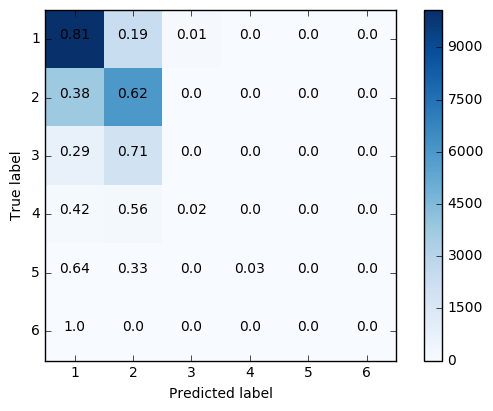
\includegraphics[width=.95\linewidth]{img/corp_lin_cm_retweets}
  \caption{Company data set}
  \label{fig:retw_distr_sub3}
\end{subfigure}%
\caption{Confusion matrices for linear retweet classification models}
\label{fig:lin_cm}
\end{figure}

More detailed observations about classification performance can be derived from
looking at confusion matrices (see Fig.~\ref{fig:lin_cm}).
These illustrations contrast predicted and actual classes for all three data sets.
For example, entry $c_{ij}$ denotes which percentage of examples in class $i$
were placed in class $j$ by the classifier.
Hence, high percentages on the main diagonal are desirable for a solid classifier.
In addition to these normalized values, color maps illustrate the absolute
number of predictions for a particular class combination.
It can be stated that all models are biased towards larger classes, i.e.,
most examples are simply placed in these classes.
For celebrities, the most common class for celebrity tweets is 4 (100-999 retweets), while classes
3 (10-99 retweets) and 0 (zero retweets) are most frequently occurring for politician and company data
(see ch.~\ref{sec:engagement_stats}).
Accuracy for predicting these popular classes is higher than 75\% on all three data sets.
However, too many examples from other classes are misclassified here, as can be
seen when looking at respective class columns.
Such model behavior results in poor predictive performance for less common classes.
Confusion matrices for favorite prediction yield similar results and are
omitted for the sake of brevity here (see Appendix).

Analyzing above results points to an intuitive interpretation of model behavior.
All models are obviously biased towards the more common classes in a data set.
Since the company data possesses the most class imbalance (nearly 90\% of examples
stem from classes 0 and 1), linear models tend to perform better here.
Contrary, model performance decreases for wider and less imbalanced class distributions.
Two possible reasons for this kind of model bias can be derived.
Firstly, linear models have limited representational capability, i.e., a small
number of trainable parameters.
Secondly, structured input features could not be sufficient to learn acceptable
class boundaries.
For example, the actual tweet content is mostly ignored when using these simple
features.
The following sections will aim to overcome these liabilities by replacing
linear models with deep neural networks.
Adding more layers to the model architecture results in more trainable parameters
for representing inputs, which in turn should improve
model performance.
Results from training deep feedforward models on structured input data are
described in the following section (ch.~\ref{sec:deep1}).
Moreover, modeling tweet content using more sophisticated layer architectures
should enable deep neural networks to learn more meaningful features.
These additional features derived from unstructured data should also enable
more accurate engagement predictions.
Ch.~\ref{sec:deep_combined} explores possibilities for building these kinds
of more complex models.


\subsection{Deep Models on Structured Data}
\label{sec:deep1}

Linear models directly map from inputs to predictions.
Assuming the inputs stay the same, the next step in neural network evolution
should be to add hidden layers.
The reasoning behind this is the increased capability of the model to learn intermediate
feature representations, which in turn should enable more accurate predictions.
This section examines application of deep feedforward networks to the problem
of engagement prediction.
Model architectures are introduced in Chapter~\ref{sub:deep1_architecture}, 
before the training process is detailled in Chapter~\ref{sub:deep1_training}.
Finally, results and accompanying analysis are presented in Chapter~\ref{sub:deep1_performance}.

\subsubsection{Model architecture}
\label{sub:deep1_architecture}

Model architecture for the deep feedforward networks is similar to linear models
in that model inputs and outputs are the same.
The main difference is the addition of hidden layers inbetween inputs and outputs.
Fully-connected feedforward layers (see ch.~\ref{sub:dl_concepts}) are chosen,
because they constitute the sole reasonably applicable layer architecture.
More complex layer architectures like recurrent or convolutional layers require
temporal or local relations between input features.
Examples for such relations would be images (local relations between pixels)
or time-series data (obvious temporal relation).
The main question that arises is how many hidden layers should be inserted.
Additionally, the number of neurons in hidden layers has to be determined.
No strict rules exist to answer this question, but heuristics have been developed
by long-time deep learning practicioners~\footnote{\url{http://www.heatonresearch.com/2017/06/01/hidden-layers.html}}.
In any case, experimentation is required to find a suitable architecture for a distinct problem setting.
Thus, several architectures were tested for model selection in this work.
Obvious evaluation criteria are model performance on training and validation data,
as well as total training time.

\begin{table}
\begin{tabular}{llrr}
\toprule
Hidden layers & Hidden units & Classification loss & Regression loss \\
\midrule
2 & 16 & 0.8203 & 2,593.2 \\
2 & 32 & 0.7502 & 2,520.2 \\
2 & 64 & 0.7346 & 2,509.9 \\
3 & 16 & 0.7888 & 2,529.9 \\
3 & 32 & 0.7430 & 2,557.3 \\
3 & 64 & 0.7160 & 2,465.1 \\
4 & 16 & 0.7792 & 2,588.5 \\
4 & 32 & 0.7261 & 2,477.5 \\
4 & 64 & \textbf{0.7088} & 2,435.8 \\
5 & 64 & 0.7128 & \textbf{2,386.1} \\
6 & 64 & 0.7016 & 2,410.1 \\
\bottomrule
\end{tabular}
\caption{Summary of model selection results}
\label{tab:dm1_selection_results}
\end{table}

Experimentation for classification and regression models was conducted on the
celebrity data set, because it contains the smallest number of training examples
and is thus most prone to overfitting.
In order to preserve comparability, the same settings were used for each architecture.
Models were trained for 50 (classification) respectively 100 (regression) epochs
on identical training examples.
Tested variants included two to six hidden layers with the same number of hidden
units in each layer, namely 16, 32 and 64 neurons.
Some architectures for very deep networks (five or six hidden layers) were omitted
when it became obvious that layers with 64 neurons showed the most promising
performance.
Table~\ref{tab:dm1_selection_results} summarizes results for the experiments.
As expected, increases in both number of hidden layers and units improve
performance.
However, adding units yields generally leads to higher performance increases than
simply adding layers.
In addition, adding more hidden layers increases total training time more than
adding units.
Including more than four hidden layers only leads to minor performance improvement for
the classification setting.
Also, a more unstable training process was observed, sometimes resulting in overfitting.
Hence, the configuration consisting of four layers with 64 neurons each was
chosen for models in this thesis.
The regression setting proved to be a bit more robust regarding the number of
hidden layers, so that an additional layer could be inserted here.

\begin{figure}[h]
\begin{subfigure}{.4\textwidth}
  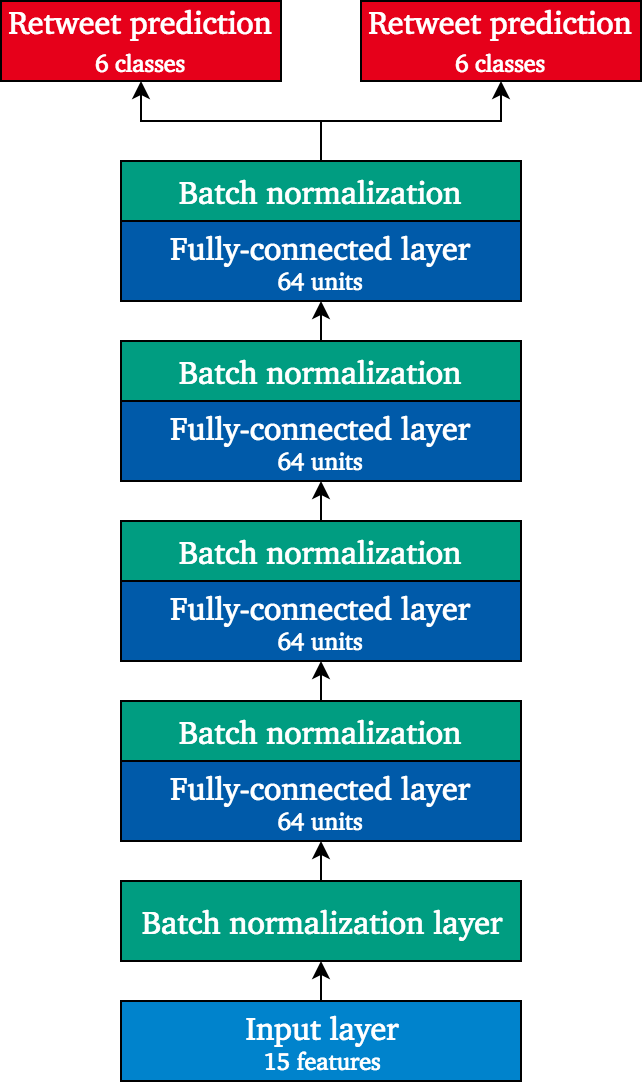
\includegraphics[width=.95\linewidth]{img/deep_1_class_architecture}
  \caption{Classification model}
  \label{fig:deep1_architecture_1}
\end{subfigure}%
\begin{subfigure}{.4\textwidth}
  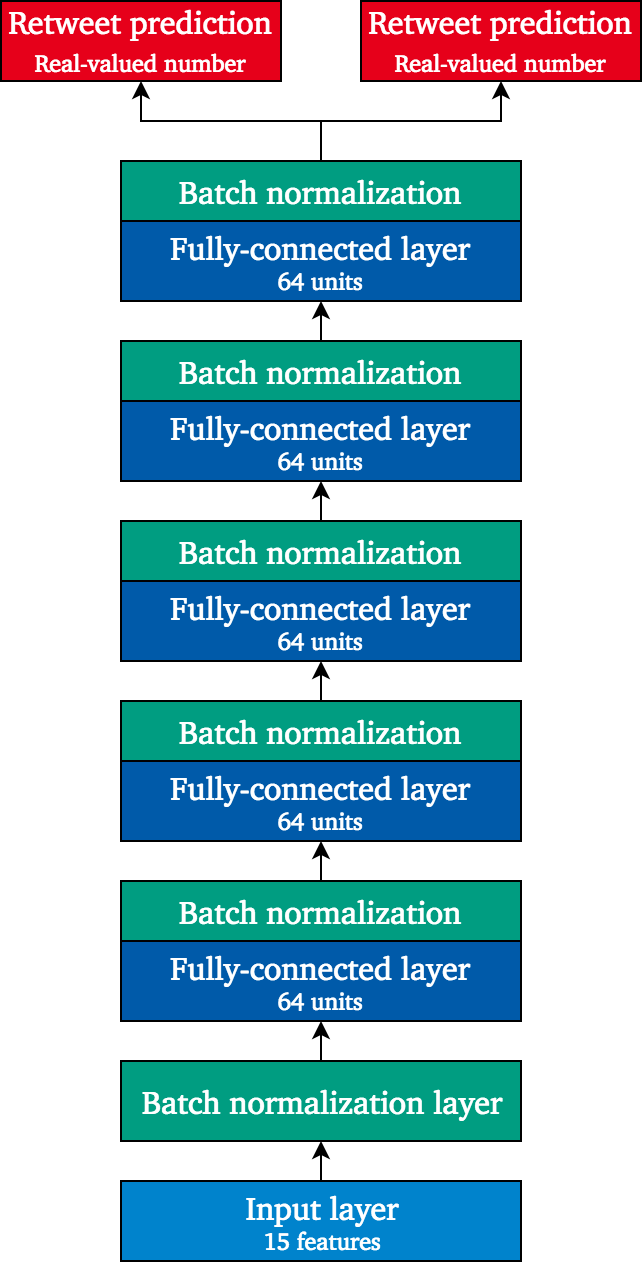
\includegraphics[width=.95\linewidth]{img/deep_1_regr_architecture}
  \caption{Regression model}
  \label{fig:deep1_architecture_2}
\end{subfigure}
\caption{Architecture of deep feedforward network}
\label{fig:deep1_architecture}
\end{figure}

Fig.~\ref{fig:deep1_architecture} shows the final neural network architectures
for this section.
Input features and output types (including classes) are identical to the ones
used in linear models (see ch.~\ref{sub:lin_architecture}).
As before, inputs are normalized using batch normalization, which is also applied
after each fully-connected layer.
Citing Chapter~\ref{sub:dl_developments}, batch normalization speeds up the
training process by decreasing the range of weight values without sacrificing
model performance.
Moreover, it helps to avoid overfitting, which is more prone to occur in models
containing many learnable parameters.

\subsubsection{Training process}
\label{sub:deep1_training}

\outline{Setting is mostly unchanged: same training/validation split, optimizer
and cost functions}
\outline{Only change: regression model trained for only 100 iterations since they
converge faster}

\subsubsection{Model performance}
\label{sub:deep1_performance}

\begin{table}
  \begin{tabular}{lrrrrrrr}
    \toprule
    & \multicolumn{4}{l}{Classification} & \multicolumn{3}{l}{Regression} \\
    \midrule
    Data set & CCE & Acc & Ret Acc & Fav Acc & MAE & Ret MAE & Fav MAE \\
    \midrule
    Celebrities & 0.71 & 70.29\% & 66.30\% & 74.28\% & 2,345.85 & 1,165.19 & 3,526.51 \\
    Politicians & 0.81 & 64.75\% & 63.37\% & 66.12\% & 424.05 & 247.40 & 600.69 \\
    Companies & 0.72 & 70.07\% & 72.38\% & 67.76\% & 19.72 & 10.92 & 28.52 \\
    Combined & 1.03 & 55.50\% & 57.75\% & 53.25\% & 549.93 & 210.71 & 889.16 \\
    \bottomrule
  \end{tabular}
  \caption{Summary of results for deep feedforward network}
  \label{tab:deep1_results}
\end{table}

\outline{Overall performance increases (cost function lower for both tasks
across all data sets)}
\outline{Additional information: models start to overfit slightly (esp. company
classification => training loss is 0.64)}
\outline{Classification accuracy improvements between 10 and 20 \% (celebrity performance
improvements are strongest), 65 to 70\% of validation examples are classified correctly}
\outline{Improvements are slightly higher for favorite classification (except for politicians)}
\outline{Relation between RetAcc and FavAcc unchanged}
\outline{Interesting: classification works best for celebrity data (previously worst performance)}
\outline{MAE results lowered by 12 (politicians) to 33\% (celebrities)}
\outline{Improvements mostly driven by strong decreases in FavMAE (decreases
higher across the board)}
\outline{More details on classification and regression performance in the following}

\begin{figure}[h]
\begin{subfigure}{.5\textwidth}
  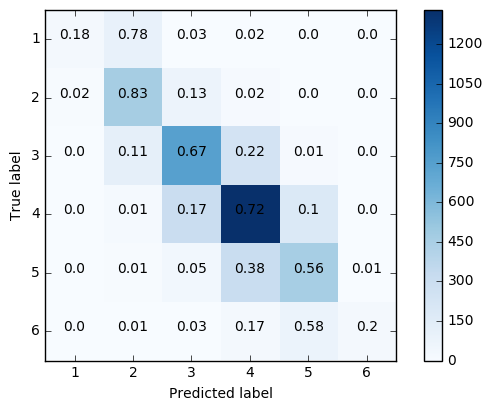
\includegraphics[width=.95\linewidth]{img/celeb_d1_cm_retweets}
  \caption{Celebrity data set}
  \label{fig:retw_distr_sub1}
\end{subfigure}%
\begin{subfigure}{.5\textwidth}
  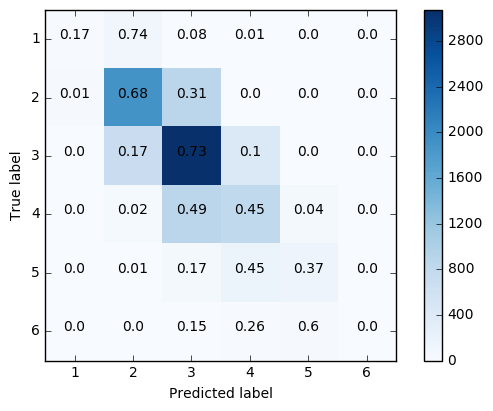
\includegraphics[width=.95\linewidth]{img/polit_d1_cm_retweets}
  \caption{Politician data set}
  \label{fig:retw_distr_sub2}
\end{subfigure}
\begin{subfigure}{.5\textwidth}
  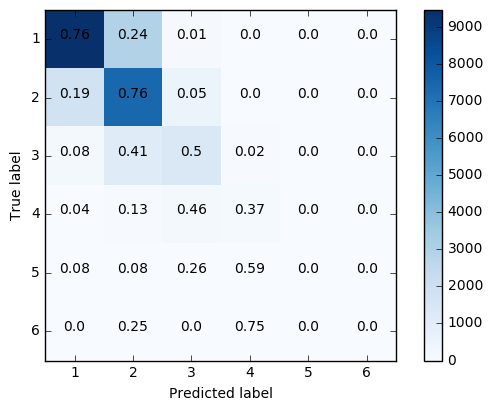
\includegraphics[width=.95\linewidth]{img/corp_d1_cm_retweets}
  \caption{Company data set}
  \label{fig:retw_distr_sub3}
\end{subfigure}%
\begin{subfigure}{.5\textwidth}
  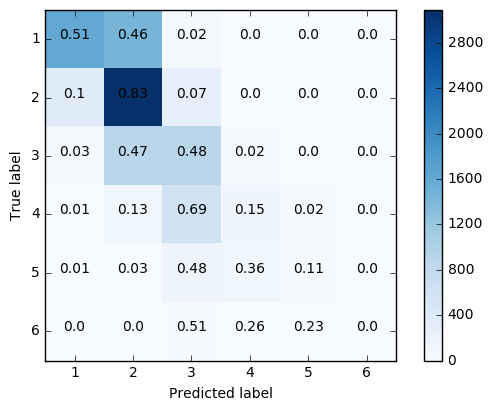
\includegraphics[width=.95\linewidth]{img/comb_d1_cm_retweets}
  \caption{Combined data set}
  \label{fig:retw_distr_sub4}
\end{subfigure}%
\caption{Confusion matrices for deep feedforward classification models}
\label{fig:d1_cm}
\end{figure}

\outline{More correctly classified examples (see main diagonal)}
\outline{Celebrities: Classes around median are predicted more accurately than border classes}
\outline{Celebrities: Not biased towards biggest class, misclassifications are `better'}
\outline{Sames is true for politicians}
\outline{Companies: model is good at predicting first two classes}
\outline{Companies: better (but not good) performance on classes 3 and 4}
\outline{Companies: classes 5 and 6 are still never predicted}

\begin{table}
  \begin{tabular}{lrrrrrrr}
    \toprule
    & \multicolumn{7}{c}{Actual retweets} \\
    \midrule
    Data set & 0 & 1-10 & 10-100 & 100-1k & 1-10k & 10-100k & >100k \\
    \midrule
    Celebrities & - & 51.9 & 161.4 & 701.3 & 3,884.9 & 21,557.9 & - \\
    Politicians & 46.0 & 109.7 & 184.5 & 781.0 & 3,973.1 & - & - \\
    Companies & 1.5 & 5.9 & 49.5 & 605.7 & - & - & - \\
    Combined & 0.4 & 5.2 & 32.0 & 233.6 & 2,088.3 & 21,919.0 & 86,217.9 \\
    \bottomrule
    \toprule
    & \multicolumn{7}{c}{Actual favorites} \\
    \midrule
    Data set & 0 & 1-10 & 10-100 & 100-1k & 1-10k & 10-100k & >100k \\
    \midrule
    Celebrities & - & 7.4 & 268.5 & 638.1 & 3,139.2 & 19,212.0 & 45,031.3 \\
    Politicians & 92.6 & 130.4 & 234.1 & 864.5 & 3,528.9 & 12,167.6 & - \\
    Companies & 6.5 & 6.6 & 39.7 & 743.1 & 1,314.0 & - & - \\
    Combined & 0.4 & 4.4 & 32.1 & 355.8 & 3,279.5 & 26,871.1 & 169,920.5 \\
    \bottomrule
  \end{tabular}
  \caption{Mean absolute errors for specific ranges of actual engagement}
  \label{tab:d1_regression_eval}
\end{table}

\outline{Using MAE requires mean calculation => need for more detailed performance
evaluation}
\outline{Errors need to be considered in relation to magnitude of actual counts}
\outline{Table shows MAE for specific ranges of actual engagement counts}
\outline{Dash denotes absence of validation data for this range}
\outline{Observation: MAE increases with rising engagement counts}
\outline{Order of magnitudes vary drastically (can be expected)}



\subsection{Deep Models on Enriched Data}
\label{sec:deep_combined}

\subsubsection{Text preprocessing}
\label{sub:text_preprocess}

\subsubsection{Model architecture}
\label{sub:model_architecture}

\subsubsection{Model performance}
\label{sub:comb_performance}

\subsection{Summary}
\label{sec:res_summary}

\chapter{Conclusion}
\label{ch:conclusion}

% Nature of main arguments
% How researched
% What discovered
% Significance
% Contribution statement

\chapter{Future work}
\label{ch:future_work}

\outline{Evolve NN architectures using automated approaches, e.g., AutoML}

\outline{Try to interpret model features}

\section{Future work}
\label{ch:future_work}

As previously mentioned in the summary of results, the methodology used in this
thesis can be evolved in many ways.

In comparison to other natural language processing research, data sets in this
work rely on a rather small collection of texts.
This effectively limits the number of patterns identifiable by the network and
thus its learning power.
Consequently, futher research in this area should be conducted using large-scale
data sets of tweets from a variety of sources.
Based on results from this thesis, a rough guideline would be a minimum
of 300,000 labeled examples of each class.
Working on larger data sets would also allow to remove class imbalances,
e.g., by applying techniques such as undersampling.
Furthermore, deeper network architectures containing more text processing
and feature combination layers could be evaluated, as overfitting is less likely
to occur on large data sets.
Another conceivable extension would be to make models work with multi-linguistic
data.
Some preconditions for this feature are already established, as GloVe word
vectors come for tokens from a variety of languages.

All hyperparameter tuning and testing of model architectures in this work was
undertaken manually.
As these processes mainly consist of executing the same set of tasks repeatedly,
they are suitable for automation.
Approaches to automatically testing different sets of hyperparameters for
machine learning models have been subject of research for quite some time~\footnote{\url{http://www.ml4aad.org/automl/}}.
Recently, these ideas were picked up by companies like Google in order to free
up human resources and allow less experiences practicioners to develop
well performing models~\footnote{\url{https://cloud.google.com/automl/}}.
Applying such techniques to models in this work could further enhance their
overall performance.

The tradeoff between model performance and interpretability is ubiquitous in
the area of machine learning.
Regulatory authorities require companies in many sectors to be able to explain
decision origins.
As mentioned previously, deep neural networks represent so-called black box models.
This means that the learned feature representations are not directly extractable
and comprehensible for humans.
Nevertheless, approaches to enhance interpretability have been established
in recent research, especially for convolutional neural networks operating
on image data (see ch.~\ref{sub:dl_architectures}).
Similar experiments have been undertaken for recurrent neural networks~\footcite{Karpathy2015}.
Future work in the area of engagement prediction using deep neural networks
should focus on incorporating such techniques in order to understand learned
model features for this task.


%\section{Einleitung}
\lbrack Zitat (optional)\rbrack :
\begin{quote}
\glqq Was ist die Absicht eines wissenschaftlichen Buches? Es stellt Gedanken dar und will den Leser von ihrer Gültigkeit überzeugen. Darüber hinaus will der Leser auch wissen: woher kommen diese Gedanken und wohin führen sie? Mit welchen Richtungen auf anderen Gebieten hängen sie zusammen?\grqq
\pcite{}{XVII}{carnap1974}
\end{quote}

Einer der wichtigsten Abschnitte der Arbeit ist die Einleitung, in der der Leser in das Thema eingeführt wird. Auch ein fachfremder Leser muss nach dem Lesen der Einleitung verstanden haben, warum das vorliegende Thema wichtig und erforschenswert ist. Die Einleitung sollte zum Weiterlesen animieren und das Interesse des Lesers wecken. Neben dieser Motivation der Arbeit sind die Zielsetzung und die Forschungsfragen der Arbeit zu konkretisieren. Diese werden im Laufe der Arbeit beantwortet. Abschließend folgt ein kurzer Überblick über die Arbeit.\par\medskip
In den folgenden Kapiteln wird ein typischer Aufbau einer wissenschaftlichen Arbeit dargestellt und jeweils anhand ihrer typischen Inhalte beschrieben. Dieser Aufbau ist jedoch nicht verbindlich und kann je nach Forschungsmethode stark variieren. Bitte klären Sie dies mit Ihrem jeweiligen Betreuer ab.\par\medskip
Nach der Einleitung (Kapitel 1) folgen die Grundlagen (Kapitel 2) und die Entwicklung eines Forschungsmodells (Kapitel 3). In Kapitel 4 wird die verwendete Forschungsmethode dargestellt und in Kapitel 5 die Forschungsergebnisse. Eine Diskussion der Ergebnisse findet in Kapitel 6 statt. Die Arbeit schließt mit einer abschließenden Zusammenfassung sowie mit einem Fazit und einem Ausblick (Kapitel 7).

%1
%\section{Grundlagen}
Im Grundlagenkapitel stellen Sie das Basiswissen für die weiteren Kapitel vor. Hierzu können neben theoretischen Konzepten auch die historische Entwicklung und aktuelle Forschungsvorhaben gehören. Idealerweise bedient man sich hier mehrerer verschiedener Quellen, um die Ausführungen zu belegen.

Nachfolgend werden einige Formalitäten der Arbeit dargestellt.

Zur korrekten Verwendung der Vorlage benötigen Sie die TU Darmstadt Schriftart: \href{https://www.tu-darm-stadt.de/kommunikation_und_medien/corporate_design_1/schriften_und_vorlagen/index.en.jsp}{Schriften und Vorlagen der TU Darmstadt}
\subsection{Gliederungen}
Text
\subsubsection{Gliederungsebene 3}
Text
\paragraph{Gliederungsebene 4}
Text
\subsection{Aufzählungen}
\begin{itemize}
	\item Fehlende Motivation,
	\item Fehlende Agilität und 
	\item Fehlende Compliance.
\end{itemize}

Text 
\newpage
\subsection{Abbildungen}

\begin{figure}[h]
\begin{center}

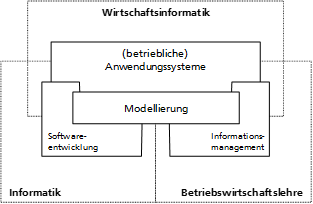
\includegraphics[width=10cm]{images/Abb2_3.png}
\caption{Einordnung der Wirtschaftsinformatik (angelehnt an Fink et al. 2001)}
\label{Abbildung2_3}
\end{center}
\end{figure}
Bitte achten Sie darauf, dass alle vorhandenen Abbildungen und Tabellen in einem inhaltlichen Zusammenhang mit dem Text stehen und Sie auf die entsprechende Abbildung (bspw. Abbildung 1) verweisen.
\subsection{Tabellen}
%hier Tabelle einfügen
\begin{table}[h]
\centering
\begin{tabular}{ccc}
\hline \textbf{Attribute} &\textbf{Typ}  & \textbf{1. Ausprägung (Beispiel)} \\ 
\hline Titel & \textit{STRING}& Aktiengesetz (AktG)  \\ 
Text& \textit{STRING} &  [Text des AktG]\\ 
Gültig von & \textit{DATE} & 01.01.2010 \\ 
Gültig bis & \textit{DATE} & - \\ 
Dok.-Besitzer & \textit{STRING} & Rechtsabteilung \\ 
Quelle & \textit{STRING}  & Deutsche Gesetze \\ 
Verplichtungsgrad & \textit{STRING} & verplichtend \\ 
\hline 
\end{tabular} 
\caption{Attribute der Anforderungsquellen im Metamodell}
\label{tab:tabelle 1}
\end{table}
\par\medskip

Tabelle 1 stellt eine beispielhafte Tabelle dar%2
%\section{Entwicklung eines konzeptuellen Rahmens}
\label{cha:entwicklung}
Dieses Kapitel dient der Entwicklung eines konzeptuellen Rahmens auf Basis theoretischer Grundlagen, vorausgesetzt sie verfolgen einen positivistischen Ansatz. Hierfür leiten Sie Hypothesen aus verschiedenen sinnvoll kombinierten Quellen her. Hierdurch generieren Sie aus bestehendem Wissen neues Wissen, was eine Eigenleistung und somit ein wichtiger Bestandteil Ihrer Arbeit darstellt.

Sollte Ihre Arbeit nicht positivistisch ausgelegt sein, stellt dieser Abschnitt kein Pflichtkapitel der Arbeit dar. Alternativ beschreiben Sie Anforderungen für ein mögliches Konzept oder verzichten vollständig auf dieses Kapitel.

\textbf{Setzen Sie sich frühzeitig mit Ihrem Betreuer in Verbindung, um Ihre Gliederung abzustimmen und mögliche Missverständnisse zu beseitigen.}

Im Folgenden werden einige allgemeine Hinweise zu den Themen richtiges Zitieren und Literaturrecherche gegeben.


\subsection{Quellen und richtiges Zitieren}
Quellen können in Fußnote oder direkt im Text platziert werden. Alles was nicht Ihr eigenes Gedankengut darstellt, muss mit einer entsprechenden Quelle belegt werden. Hierbei können wörtliche und indirekte Zitate verwendet werden. Wörtliche Zitate sind immer mit der Seitennummer der Quelle anzugeben.

Beispiel für ein direktes Zitat:

\textit{\glqq The case study is a research strategy which focuses in understanding the dynamics present within single settings\grqq} \pcite{}{543}{eisenhardt1989}.

Beispiel für ein indirektes Zitat:

Eine explorative Fallstudie dient der Gewinnung von neuen Erkenntnissen und der Bildung von neuen Hypothesen über bestimmte Sachverhalte. Durch den Beitrag zum Theorieaufbau ist der Erkenntnisgewinn höher als bei einer reinen deskriptiven Fallstudie. In explorativen Fallstudien werden Phänomene in noch wenig erforschten Gebieten identifiziert und aus erkannten Zusammenhängen neue Hypothesen gebildet \citepara{eisenhardt1989}.

Alternativ kann die Quelle auch im  laufenden Text angegeben werden:

Nach \citeflow{eisenhardt1989} wird die Wichtigkeit der Fallauswahl oft unterschätzt. Die Fälle können zwar zufällig ausgewählt werden, dies ist aber weder notwendig noch wünschenswert.

Quellenangaben bestehen aus Autor, Jahr und ggf. Seitenangabe. Bei zwei Autoren sind beide Autoren zu nennen, bei mehreren Autoren nur der erste Autor mit dem Zusatz „et al.“.\newpage


\subsection{Zitieren mit Endnoten}
Im Rahmen der Erstellung von Arbeiten am Fachgebiet ISE ist das Literaturverwaltungsprogramm EndNote zu verwenden. Dieses steht auf der \href{http://www.ulb.tu-darmstadt.de/service/literaturverwaltung_start/endnote_ulb/endnote.de.jsp
}{ULB-Seite} zum Download verfügbar. 


\subsubsection{Lateinischer Text mit Zitaten für Erstellung des Literaturverzeichnisses}
\label{cha:source:latintext}
Lorem ipsum dolor sit amet, consectetur adipiscing elit. Sed vitae lacus eu augue semper lobortis vitae aliquet leo. Fusce eleifend sodales commodo \citepara{eisenhardt1989}. Mauris arcu metus, bibendum sagittis condimentum eget, placerat a enim \citepara{baechle2010}. Quisque sit amet sagittis lectus. Curabitur sit amet libero eu felis elementum mollis. Nullam odio diam, mollis vitae viverra ut, laoreet ut odio. Praesent facilisis suscipit consequat. Morbi feugiat rutrum erat, eu sagittis nibh rhoncus nec \citepara{melao2000}.

In euismod, arcu ut semper adipiscing, nibh odio ullamcorper arcu, ut scelerisque massa magna nec quam \citepara{benlian2013}. Curabitur bibendum nibh eget augue pellentesque iaculis \citepara{sheffi2005}. Praesent iaculis auctor gravida. Quisque congue, magna ut bibendum semper, enim tortor ultrices lorem, ac feugiat tortor lectus nec nunc \citepara{carnap1974}. Pellentesque habitant morbi tristique senectus et netus et malesuada fames ac turpis egestas. Lorem ipsum dolor sit amet, consectetur adipiscing elit. Fusce dignissim, augue a sodales tristique, neque dui mollis arcu, id interdum augue justo sed lacus \citepara{welchering2013}. Vestibulum ante ipsum primis in faucibus orci luctus et ultrices posuere cubilia Curae; Mauris euismod bibendum nulla, sed accumsan urna tempor sed. Etiam eget diam eros, sed aliquet dolor \citepara{broadbent1996}. Phasellus vitae quam in orci convallis pharetra. Donec sit amet imperdiet nisi \citepara{kayser2013}. Sed vel interdum orci. Praesent vulputate, dolor id varius egestas, enim libero cursus neque, a cursus sapien nulla ut augue. Nullam vitae tortor nisl, vitae cursus enim. Suspendisse eget metus ipsum, sit amet varius sem \citepara{shazly2013}.

\subsection{Literaturrecherche}
Anbei eine kurze Auflistung von möglichen Kanälen zur Literaturrecherche.

\textbf{Zu Verwaltung Ihrer Literatur benutzen Sie bitte das Programm EndNote, dieses wird kostenfrei von der TU zu Verfügung gestellt.}

\url{http://www.ulb.tu-darmstadt.de/angebot/service/literaturverwaltung/endnote.de.jsp}

\subsubsection{Angebot der ULB}
\begin{itemize}
\item Universitätsbibliotheken (\url{http://www.ulb.tu-darmstadt.de/})
\item Rechercheangebot der ULB (\url{http://www.ulb.tu-darmstadt.de/recherche/})
\end{itemize}

\subsubsection{Online-Datenbanken und -Bibliotheken}
\begin{itemize}
\item Elektronische Zeitschriftenbibliothek (EZB) \\
(\url{http://rzblx1.uni-regensburg.de/ezeit/fl.phtml?bibid=TUDA})
\item AIS Electronic Library (AISeL)\\
(\url{http://aisel.aisnet.org/})
\item Zeitschriftendatenbank (ZDB)\\
(\url{http://dispatch.opac.ddb.de/DB=1.1/srt=YOP/})
\item Datenbank-Infosystem (DBIS): Literatur- und Fakten-Datenbank\\
(\url{http://rzblx10.uni-regensburg.de/dbinfo/fachliste.php?bib_id=tud})
\item IEEE Xplore \\
(\url{http://ieeexplore.ieee.org/Xplore/dynhome.jsp?tag=1})
\item EBSCO: internationale wirtschafts-wiss. Zeitschriften\\ (\url{http://search.ebscohost.com})
\item Springer-Online: Bücher/Beiträge des Springer Verlags\\
(\url{http://www.springerlink.com})
\item WiSo Net: deutschsprachige Literatur zu Wirtschafts- und Sozialwissenschaften\\
(\url{www.wiso-net.de})

\end{itemize}

\subsubsection{Sonstiges}
\begin{itemize}
\item \textbf{Google Scholar:} Suchdienst für wissenschaftliche Recherchen (http://scholar.google.de)
\item \textbf{Verlagswebseiten} Recherche und den Zugriff auf Zeitschriften- und Zeitungsartikel und E-Books
\item \textbf{Webseiten von Unternehmen} für die Recherche von Unternehmensdaten und-statistiken sowie Unternehmensdatenbanken
\item \textbf{Webseiten von Bundes- und Landesbehörden sowie der EU}
 Statistisches Bundesamt (http://www.destatis.de)
\\Presse- und Informationsamt der Bundesregierung (http://www.bundesregierung.de)
\item \textbf{Webseiten von Marktforschungsinstituten}
(für Marktanteile und Verbraucheranalysen)
\item \textbf{Webseiten von Verbänden und Kammern}
Institut der deutschen Wirtschaft (http://www.deutsche-wirtschaft.de)
\end{itemize}%3
%\section{Forschungsmethoden}
\label{cha:method}
In diesem Kapitel erläutern Sie ihre Forschungsmethode unter Verwendung von entsprechenden Quellen. Begründen Sie auch, warum Sie sich für diese Forschungsmethode entschieden haben und warum sie geeignet ist, die vorliegende Forschungsfrage zu beantworten.%4
%\section{Forschungsergebnisse}
\label{cha:result}
In Kapitel „Forschungsergebnisse“ stellen Sie die Ergebnisse ihrer Arbeit dar. An dieser Stelle nehmen Sie noch keine Interpretation oder Erläuterung der Ergebnisse vor, sondern beschreiben rein deskriptiv ihre Befunde. Eine Auswertung findet im nachfolgenden Kapitel statt.%5
%\section{Diskussion}
\label{cha:diskussion}
Im vorletzten Abschnitt diskutieren Sie Ihre Ergebnisse und stellen den Beitrag für die Praxis und für die Forschung dar. Gehen Sie auch auf die Einschränkungen Ihrer Arbeit ein.%6
%%\addtocontents{toc}{\protect\newpage}
\section{Zusammenfassung und Ausblick}
\label{cha:fazit}
% Wohin sind wir gekommen
Zuletzt fassen Sie Ihre Arbeit kurz zusammen und stellen Ihre wichtigsten Schritte, Ergebnisse und Befunde dar. Geben Sie auch einen Ausblick auf mögliche anknüpfende Forschungsarbeiten. Außerdem findet sich hier Platz für eine kritische Hinterfragung einzelner Teilaspekte und auch für Ihre eigene Meinung.

\subsection{Abgabedokument}
% Was wurde in der Arbeit alles gemacht
% Roten Faden aufgreifen
% TODO Pr�sens oder Pr�teritum
\textbf{Abschlussarbeiten} (Bachelor-, Master-, Diplomarbeit) sind in zweifacher Ausführung, ein-seitig bedruckt und gebunden abzugeben. Dazu auf CD die Abschlussarbeit in digitaler Form (z.B. Word und PDF), inkl. der Endnote-Projektdatei und der Grafiken. \par\medskip
Für \textbf{Seminar- und Studienarbeiten} genügt eine ungebundene einfache Ausführung, ebenfalls einseitig bedruckt. Die Seminar-/Studienarbeit in digitaler Form inkl. der Endnote Projektdatei sind zusätzlich per E-Mail einzureichen.

\pagenumbering{Roman}
\bibliography{bibliography/thesis}

%
%
%
%Appendix
%
%

\appendix

\section{Appendix}
\label{ch:appendix}

\subsection{User groups}
\label{sec:user_groups}

A detailed list of all examined Twitter accounts is omitted here for the sake
of brevity.
User groups were assembled as Twitter lists in the author's profile.
Find links to all lists in the following:

\begin{enumerate}
\item Celebrity user group: \url{https://twitter.com/_fpeters/lists/celebrities}
\item Politician user group: \url{https://twitter.com/_fpeters/lists/us-politicians}
\item Company user group: \url{https://twitter.com/_fpeters/lists/fortune-500}
\end{enumerate}

\subsection{Confusion matrices}
\label{sec:confusion_matrices}

Confusion matrices for favorite classification were omitted in the results chapter.
They are displayed in the following.

\begin{figure}[h]
\begin{subfigure}{.4\textwidth}
  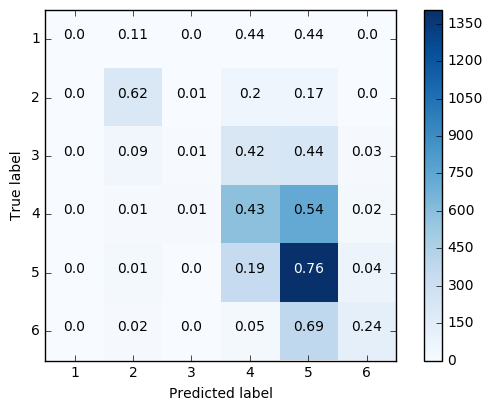
\includegraphics[width=.95\linewidth]{img/celeb_lin_cm_favorites}
  \caption{Celebrity data set}
  \label{fig:lin_fav_distr_sub1}
\end{subfigure}%
\begin{subfigure}{.4\textwidth}
  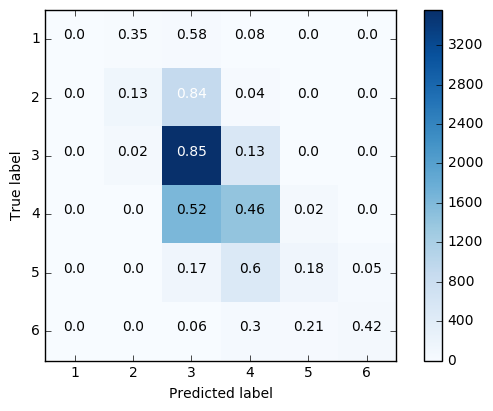
\includegraphics[width=.95\linewidth]{img/polit_lin_cm_favorites}
  \caption{Politician data set}
  \label{fig:lin_fav_distr_sub2}
\end{subfigure}
\begin{subfigure}{.4\textwidth}
  \includegraphics[width=.95\linewidth]{img/corp_lin_cm_favorites}
  \caption{Company data set}
  \label{fig:lin_fav_distr_sub3}
\end{subfigure}%
\begin{subfigure}{.4\textwidth}
  \includegraphics[width=.95\linewidth]{img/comb_lin_cm_favorites}
  \caption{Combined data set}
  \label{fig:lin_fav_distr_sub3}
\end{subfigure}%
\caption{Confusion matrices for linear retweet classification models}
\label{fig:lin_fav_cm}
\end{figure}

\begin{figure}[h]
\begin{subfigure}{.4\textwidth}
  \includegraphics[width=.95\linewidth]{img/celeb_d1_cm_favorites}
  \caption{Celebrity data set}
  \label{fig:d1_fav_distr_sub1}
\end{subfigure}%
\begin{subfigure}{.4\textwidth}
  \includegraphics[width=.95\linewidth]{img/polit_d1_cm_favorites}
  \caption{Politician data set}
  \label{fig:d1_fav_distr_sub2}
\end{subfigure}
\begin{subfigure}{.4\textwidth}
  \includegraphics[width=.95\linewidth]{img/corp_d1_cm_favorites}
  \caption{Company data set}
  \label{fig:d1_fav_distr_sub3}
\end{subfigure}%
\begin{subfigure}{.4\textwidth}
  \includegraphics[width=.95\linewidth]{img/comb_d1_cm_favorites}
  \caption{Combined data set}
  \label{fig:d1_fav_distr_sub4}
\end{subfigure}%
\caption{Confusion matrices for deep feedforward classification models}
\label{fig:d1_fav_cm}
\end{figure}

\begin{figure}[h]
\begin{subfigure}{.4\textwidth}
  \includegraphics[width=.95\linewidth]{img/celeb_d2_cm_favorites}
  \caption{Celebrity data set}
  \label{fig:d2_fav_distr_sub1}
\end{subfigure}%
\begin{subfigure}{.4\textwidth}
  \includegraphics[width=.95\linewidth]{img/polit_d2_cm_favorites}
  \caption{Politician data set}
  \label{fig:d2_fav_distr_sub2}
\end{subfigure}
\begin{subfigure}{.4\textwidth}
  \includegraphics[width=.95\linewidth]{img/corp_d2_cm_favorites}
  \caption{Company data set}
  \label{fig:d2_fav_distr_sub3}
\end{subfigure}%
\begin{subfigure}{.4\textwidth}
  \includegraphics[width=.95\linewidth]{img/comb_d2_cm_favorites}
  \caption{Combined data set}
  \label{fig:d2_fav_distr_sub4}
\end{subfigure}%
\caption{Confusion matrices for multi-input deep neural networks}
\label{fig:d2_fav_cm}
\end{figure}


\end{document}

